\documentclass[12pt]{article}
\usepackage[text={6.5in,8.50in},centering]{geometry}
\geometry{letterpaper}   
\usepackage{graphicx}
\usepackage{subfigure}
\usepackage{setspace}
\usepackage{textcomp}
\usepackage{amsmath}
\usepackage{amssymb}
\usepackage{epstopdf}
\usepackage{textcomp}
\usepackage{multirow}
\usepackage{booktabs}
\usepackage{setspace}
\usepackage{listings}
\usepackage{color}
\usepackage{enumitem}
\definecolor{codegreen}{rgb}{0,0.6,0}
\definecolor{codegray}{rgb}{0.5,0.5,0.5}
\definecolor{codepurple}{rgb}{0.58,0,0.82}
\definecolor{backcolour}{rgb}{0.95,0.95,0.92}
\lstdefinestyle{mystyle}
{
    backgroundcolor=\color{backcolour},   
    commentstyle=\color{codegreen},
    keywordstyle=\color{magenta},
    numberstyle=\tiny\color{codegray},
    stringstyle=\color{codepurple},
    basicstyle=\footnotesize,
    breakatwhitespace=false,         
    breaklines=true,                 
    captionpos=b,                    
    keepspaces=true,                 
    numbers=left,                    
    numbersep=5pt,                  
    showspaces=false,                
    showstringspaces=false,
    showtabs=false,                  
    tabsize=2
}
\lstset{style=mystyle}
\DeclareGraphicsRule{.tif}{png}{.png}{`convert #1 `dirname #1`/`basename #1 .tif`.png}
\newcommand{\q}[1]{``#1''}
\usepackage[english]{babel}
\usepackage[autostyle]{csquotes}
\date{}                 
\doublespacing



\begin{document}
\begin{center}
    \text{\bf \LARGE Machine Learning for Trading} \\[5pt]
    %\text{\bf \Large Take-Home Exam} \\[10pt]
    %\text{\large Changheng Chen}
\end{center}

\noindent
MC1. Manipulating Financial Data in Python (Python for Finance, Hilpish)\\
\noindent
MC2. Computational Investing (What Hedge Funds Really Do, Romero and Balch) \\
\noindent
MC3. Learning Algorithms for Trading (Machine Learning, Mitchell) 

%%%%%%%%%%%%%%%%%%%%%%%%%%%%%%%%%%%%%%%%%%%%%%%%%%%%%%%
\section{Manipulating Financial Data in Python}
%===================================================================================
\textcolor{white}{.} \\[-15pt]
\noindent
{\large\bf 1.0 \textcolor{white}{.} Introduction} \\ [5pt]
Python for financial applications? \\
(1) Quickly prototype algorithms \\
(2) Computational speed \\ [5pt]
\noindent
Features \\
(1) Strong scientific libraries \\
(2) Strongly maintained \\
(3) Fast (if you can stick to matrices notation because lower levels are returned in C)

%===================================================================================
\subsection{Reading and plotting stock data}

\subsubsection{What a CSV file looks like?} 
\begin{figure}[!ht]
\centering
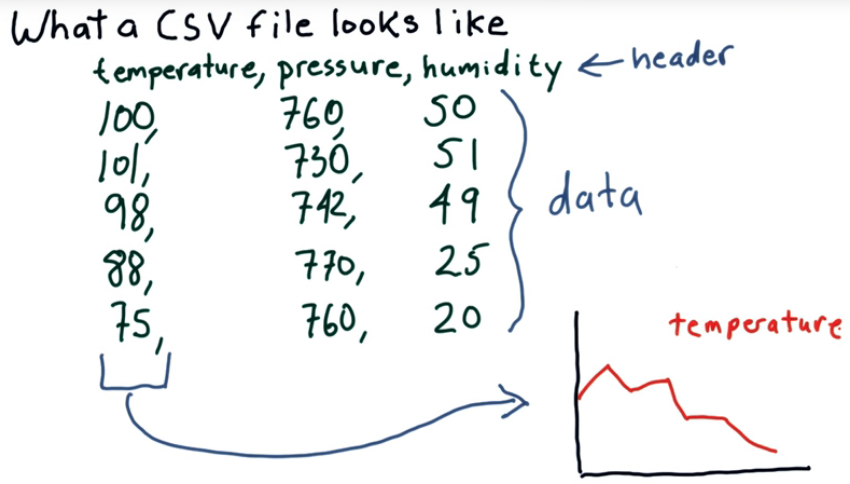
\includegraphics[scale=0.3]{fig/fig1}
\caption{Example of a CSV file}
\end{figure}

\subsubsection{Real stock data looks like this}
\begin{figure}[!ht]
\centering
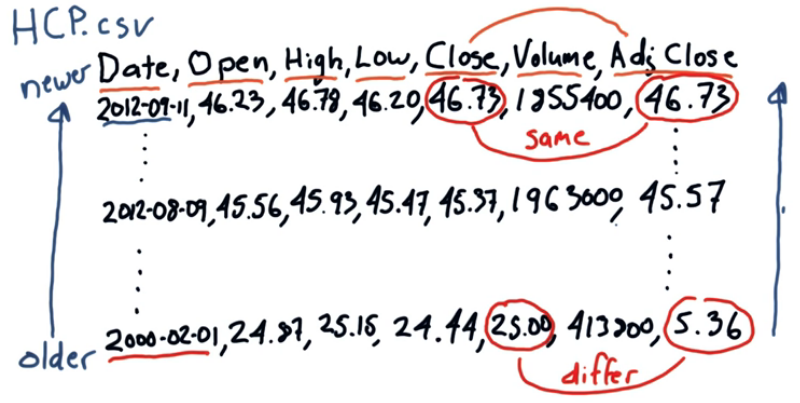
\includegraphics[scale=0.4]{fig/fig2}
\caption{Real stock data CSV file}
\end{figure}

Close: actual price that was reported at the exchange when the stock closed for that day.

Adj Close: a number that the data provider generates for us; it is adjusted for certain things like stocks, splits, and dividend payments.

\subsubsection{Pandas dataframe} 
\q{Pandas} library is created by Wes Mckinney at AQR!\\
\noindent
\q{SPY} is an ETF representing the S\&P500.
\begin{figure}[!ht]
\centering
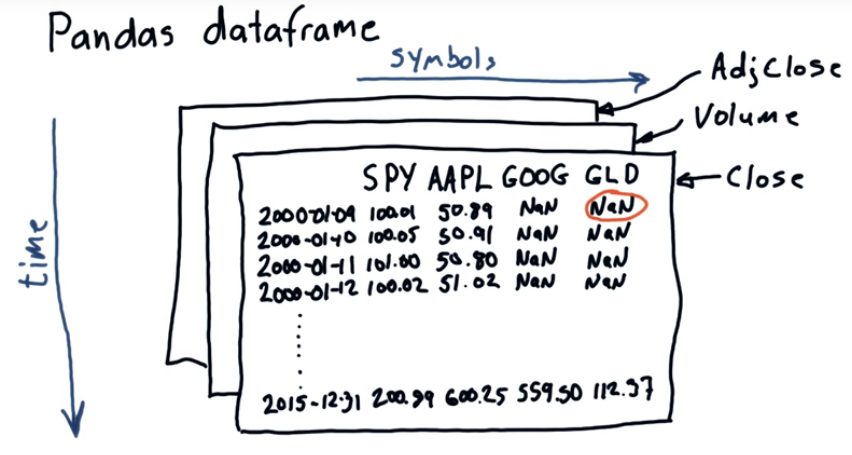
\includegraphics[scale=0.45]{fig/fig3}
\caption{Pandas dataframe}
\end{figure}

%===================================================================================
\subsection{Working with multiple stocks}

\subsubsection{Pandas dataframe} 

Problems to solve: \\
(1) Date ranges\\
(2) Multiple stocks\\
(3) Align dates\\
(4) Proper date order 

\begin{figure}[!ht]
\centering
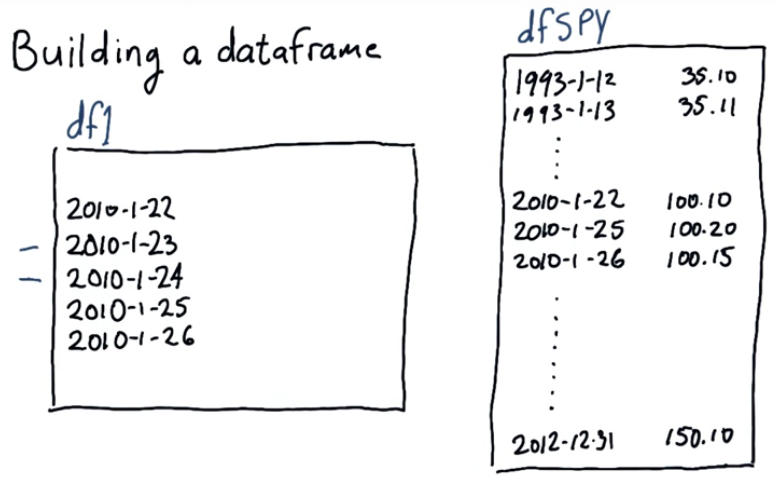
\includegraphics[scale=0.45]{fig/fig4}
\caption{Building a dataframe}
\end{figure}

S\&P 500 is a stock market index based on 500 large American companies listed on the NYSE or NASDAQ. Think of it as a weighted mean of the stock prices of the companies, where the number of shares are used as weights (with some adjustment for any events that may affect apparent stock value, such as splits).

SPDR\textsuperscript\textregistered\, S\&P 500 is an ETF (or exchange-traded fund) that tracks the S\&P 500 index, and is itself listed on NYSE under the ticker symbol \q{SPY}.

\subsubsection{Slicing dataframes}
\begin{figure}[!ht]
\centering
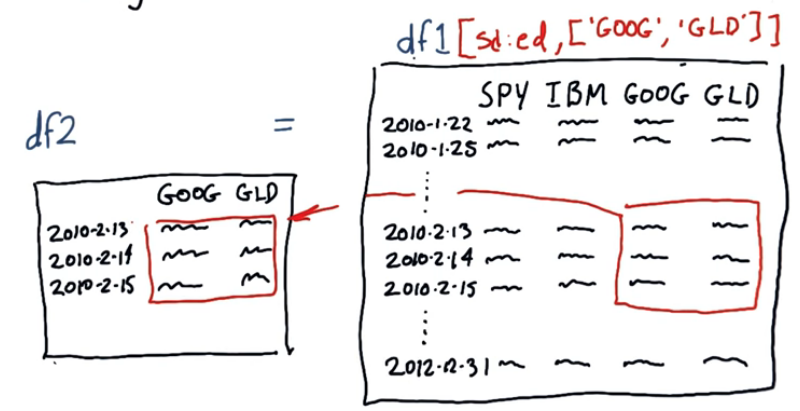
\includegraphics[scale=0.45]{fig/fig5}
\caption{Slicing dataframes}
\end{figure}

\begin{lstlisting}[language=Python, caption=]
# Quiz: What is the best way to normalize price data, so that all prices start at 1.0?
for date in df1.index:
    for s in symbols:
        df1[date, s] = df1[date, s]/df1[0, s]

df1 = df1/df1[0] # Best, faster (executed in C)
\end{lstlisting}
 
\subsubsection{Plotting a dataframe}
\begin{figure}[!ht]
\centering
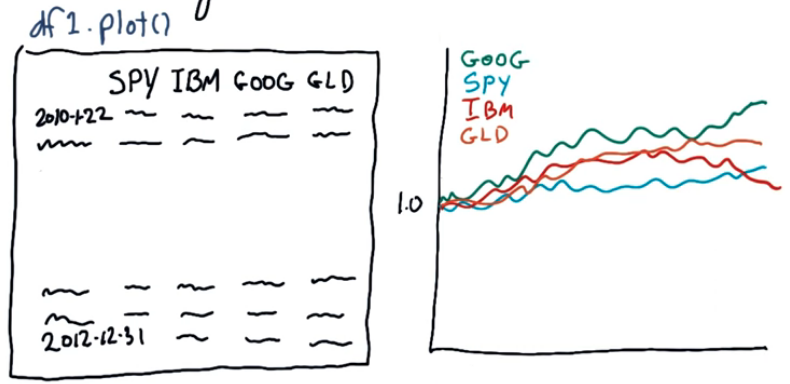
\includegraphics[scale=0.45]{fig/fig6}
\caption{Plotting a dataframe}
\end{figure}

%===================================================================================
\subsection{The power of NumPy}

\subsubsection{NumPy's relationship to Pandas}

NumPy is a Python library that acts as a wrapper around underlying C and Fortran code.

Pandas is a kind of wrapper for NumPy.

\begin{lstlisting}[language=Python, caption=]
nd1 = df1.values # pulls out the data from the df as ndarray
""" You don't have to do this you can just treat a data frame like a NumPy ndarray.
If you create a data frame instead of ndarray, you get many many more routines, a vast new number of statistical functions etc. """
\end{lstlisting}

\begin{figure}[!ht]
\centering
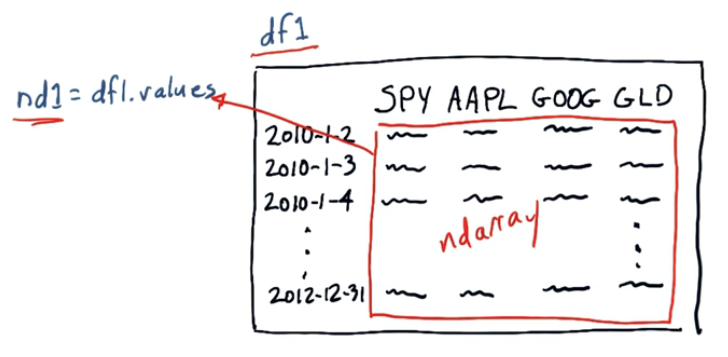
\includegraphics[scale=0.4]{fig/fig7}
\caption{This dataframe is just a wrapper around this ndarray.}
\end{figure}

\subsubsection{Notes on notation}

\begin{lstlisting}[language=Python, caption=]
"""You can access the underlying NumPy array within a Pandas data frame, using the values property OR you can create ndarray from scratch."""
nd1[row, col]
\end{lstlisting}

\begin{figure}[!ht]
\centering
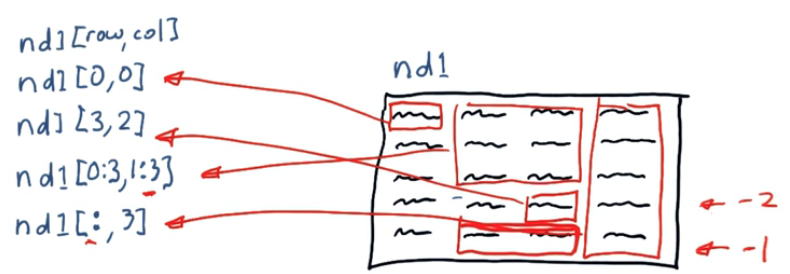
\includegraphics[scale=0.45]{fig/fig8}
\caption{Slicing ndarray}
\end{figure}

%===================================================================================
\subsection{Statistical analysis of time series}

\subsubsection{Global statistics}
\begin{lstlisting}[language=Python, caption=]
stat = df1.mean() # mean of each column
# 33 global statistics: mean, median, std, sum, prod, mode, etc.
\end{lstlisting}

\begin{figure}[!ht]
\centering
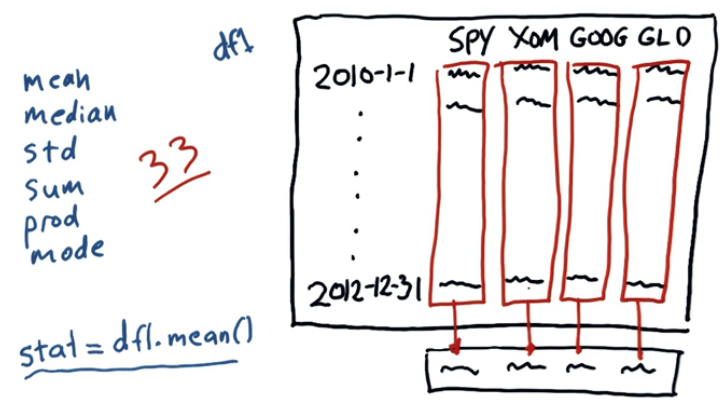
\includegraphics[scale=0.45]{fig/fig9}
\caption{Global statistics}
\end{figure}

\subsubsection{Rolling statistics}
\begin{figure}[!ht]
\centering
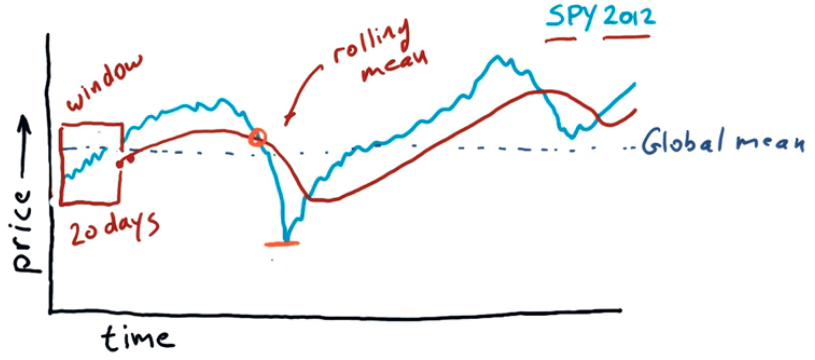
\includegraphics[scale=0.45]{fig/fig10}
\caption{Rolling statistics}
\end{figure}

\begin{lstlisting}[language=Python, caption=]
Hypothesis: rolling mean may be a good representation of sort of the true underlying price of a stock, and that significant deviations from that (e.g. the one dip in the figure eventually result in a return to the mean). So if you can look for significant deviations like this one, you might find a buying opportunity here. A challenge though, is to know when is that deviation significant enough that you should pay attention to. 
\end{lstlisting}

Quiz: How can we know a deviation from the rolling mean is significant enough to warrant a trading signal?

We need some way of measuring that. Measures of deviation: rolling standard deviation, Bollinger Bands\textsuperscript\textregistered.

\subsubsection{Bollinger Bands\textsuperscript\textregistered}
\begin{figure}[!ht]
\centering
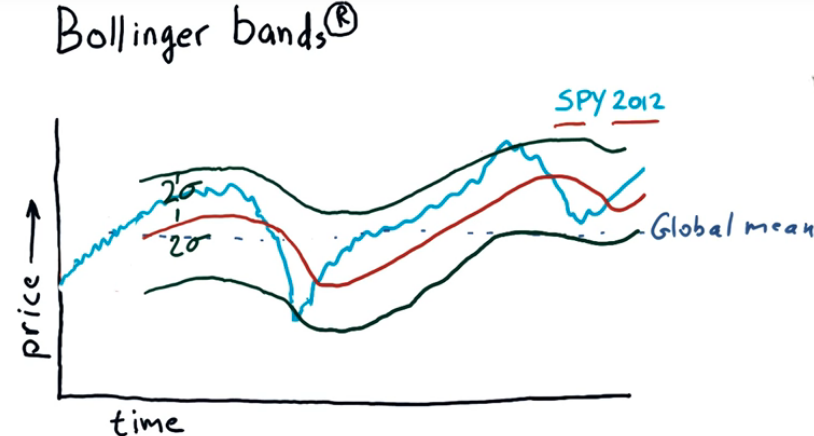
\includegraphics[scale=0.45]{fig/fig11}
\caption{Bollinger Bands\textsuperscript\textregistered}
\end{figure}

\begin{lstlisting}[language=Python, caption=]
Bollinger observed that we ought to take a look at the recent volatility of the stock:
if it is very volatile, we might discard movements above and below the mean; whereas if it is not volatile, a similarly sized movement, maybe we should pay attention to.
\end{lstlisting}

\begin{lstlisting}[language=Python, caption=]
Idea: 
To add a band $2\sigma$ above and $2\sigma$ below (how effective this method is?)
\end{lstlisting}

\begin{lstlisting}[language=Python, caption=]
Theory:
When you see excursions up to $2\sigma$  away from the mean, you should pay attention. In particular, if we drop below that and up back through it, that is potentially \textcolor{red}{a buy signal}. (Because the hypothesis is that, we have gone quite far from the simple moving average.)

if you buy there, you should anticipate positive returns as it climbs back through the average.

Similarly, where you see it punch through the top and then go back down through, that potentially \textcolor{red}{a sell signal}.

Ideally if we buy at the buy signal and then sell at the sell signal, we will do great. But many many examples are not.
\end{lstlisting}

\noindent
This is jus a technical indicator, that you might involve it in a trading strategy.

\subsubsection{Daily returns and cumulative returns}

\begin{lstlisting}[language=Python, caption=]
Daily Return: how much did the price go up or down on a particular day.

daily_ret[t] = (price[t] - price[t-1])-1
\end{lstlisting}

\begin{figure}[!ht]
\centering
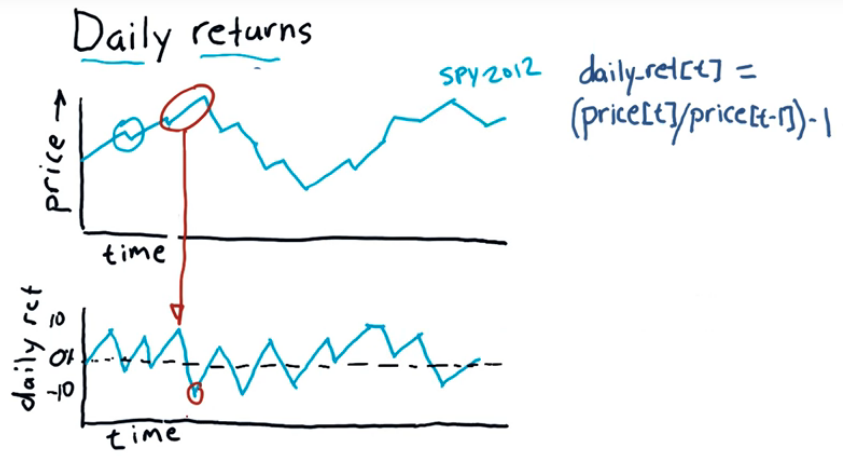
\includegraphics[scale=0.45]{fig/fig12}
\caption{Daily returns}
\end{figure}

\begin{lstlisting}[language=Python, caption=]
The year 2012 S&P 500 gained 13.6\%.

cum_ret[t] = (price[t] - price[0])-1 # cum_ret is normalized price
\end{lstlisting}

\begin{figure}[!ht]
\centering
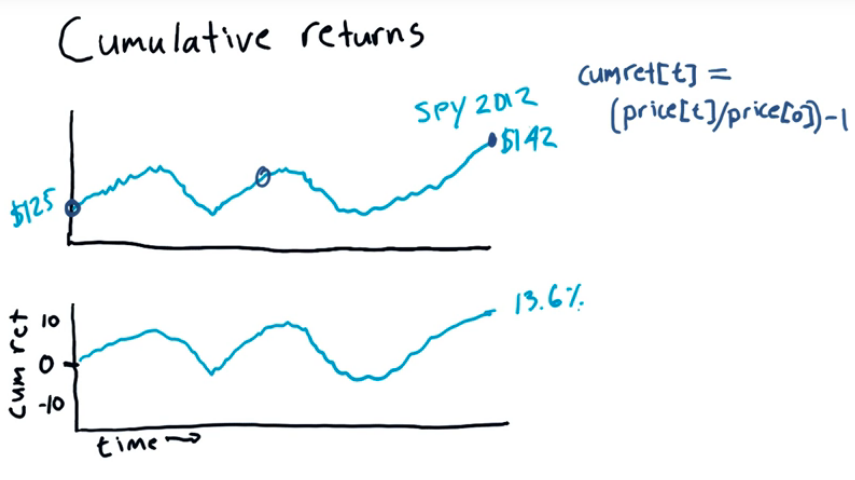
\includegraphics[scale=0.45]{fig/fig13}
\caption{Cumulative returns}
\end{figure}

%===================================================================================
\subsection{Incomplete data}

\subsubsection{Pristine data?} 
\noindent
What people think: \\
---Perfect data recorded minute by minute \\
---No gaps of missing data points

\noindent
Reality: \\
---Data is an amalgamation (created from many sources--a stock may be traded at NYSE, NASDAQ, Bats, etc., it may trade at different prices at different stock exchanges at the same time)\\
---Not all stocks trade everyday (stocks come to existence, go out of existence, then start trading again) 

\subsubsection{Why data go missing?} 

SPY: S\&P 500, one of the most liquid and actively traded ETFs (exchange traded funds), is time reference of trading (est. 1993).

(1) Sun Microsystems (trading ticker JAVA) was acquired by Oracle in 2010, and on that date JAVE went away.

(2) FAKE1 came to existence; FAKE2 existed then disappeared, then exists again---most likely are thinly traded stock (not very liquid, very large stock like Google), companies that do not have a high market capitalization, and they trade very little if at all occasionally.

\begin{figure}[!ht]
\centering
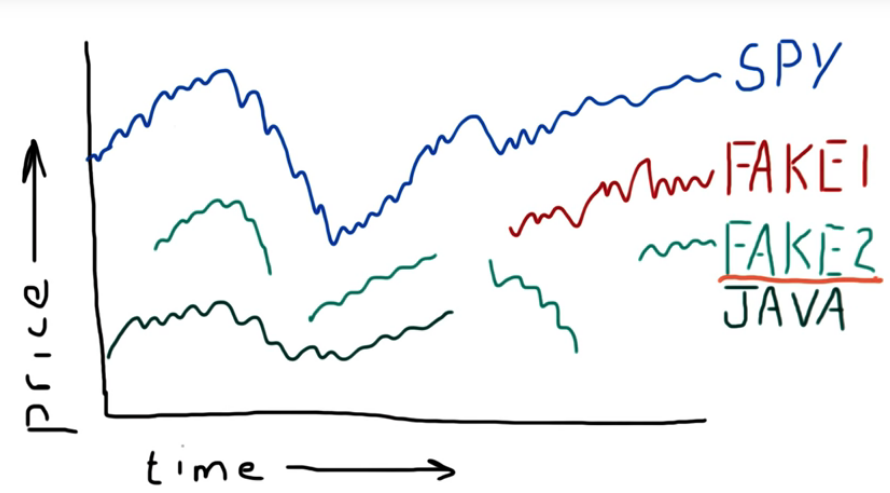
\includegraphics[scale=0.25]{fig/fig14}
\caption{Why data go missing?}
\end{figure}

\noindent
What can we do? \\
Not interpolation, not moving average! \\
We fill forward starting from the last, previous known value.

\begin{lstlisting}[language=Python, caption=]
Resolve data gaps
(1) Fill forward first
(2) Fill backward second
This will avoid "peaking" into the future

df_data.fillna(method='ffill') # fill forward
df_data.fillna(method='bfill') # fill backward
\end{lstlisting}

\begin{figure}[!ht]
\centering
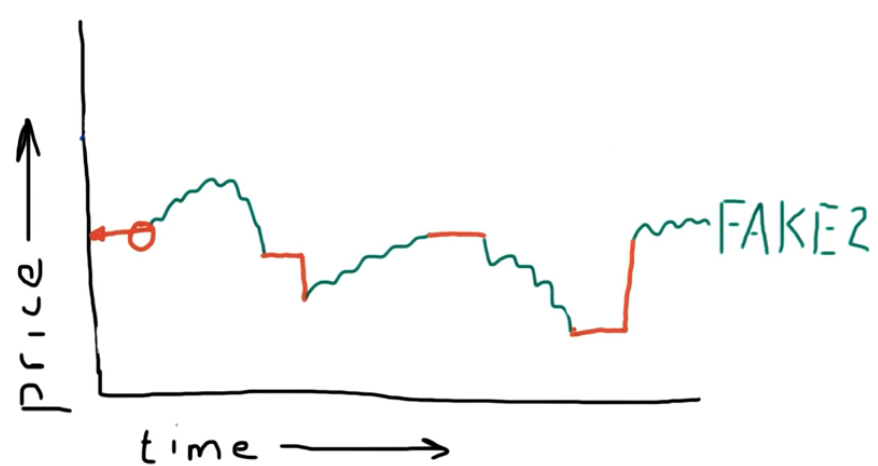
\includegraphics[scale=0.25]{fig/fig15}
\caption{Fill missing data}
\end{figure}

%===================================================================================
\subsection{Histograms and scatter plots}

\subsubsection{Hist} 

Typical hist plot: Gaussian/normal distribution (mean, std, kurtosis)

Kurtosis (curved or arching) tells us about the tails of the distribution.

\begin{figure}[!ht]
\centering
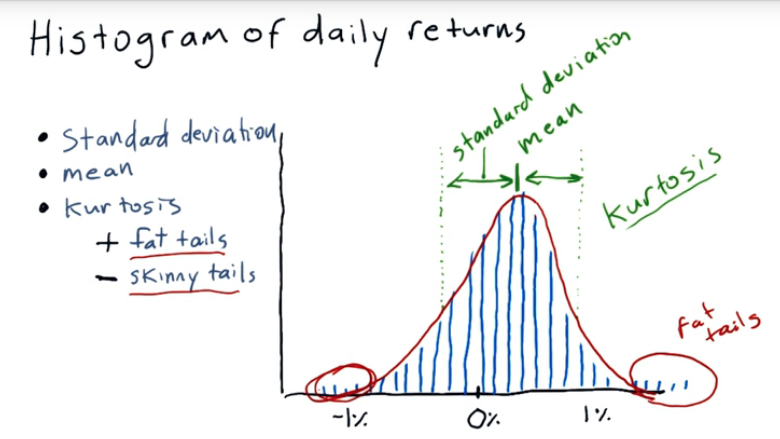
\includegraphics[scale=0.45]{fig/fig16}
\caption{Hist plot}
\end{figure}

\subsubsection{Scatter} 
\noindent
(1) correlation: a measure of how tightly do those dots fit the line \\
(2) $\beta$ (slope): how reactive the stock to the market (if $\beta$=1, an increase of 1\% of the market means an increase of 1\% of the stock) \\
(3) $\alpha$: intersect with the y-axis (positive: the stock on average performing a little better than the S\&P 500 everyday; negative: stock returns are less than the market) \\
slope $\neq$ correlation\\

\begin{figure}[!ht]
\centering
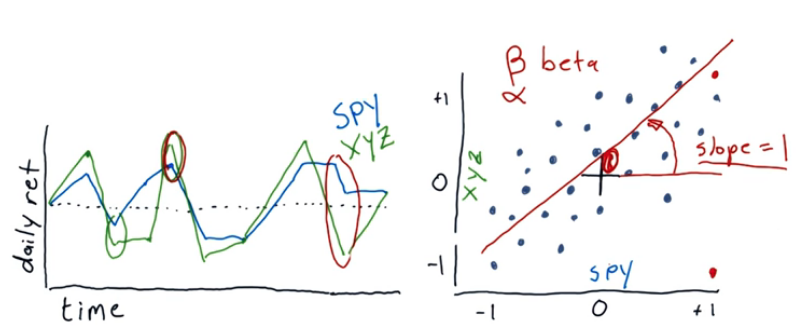
\includegraphics[scale=0.45]{fig/fig17}
\caption{Scatter plot}
\end{figure}

\begin{figure}[!ht]
\centering
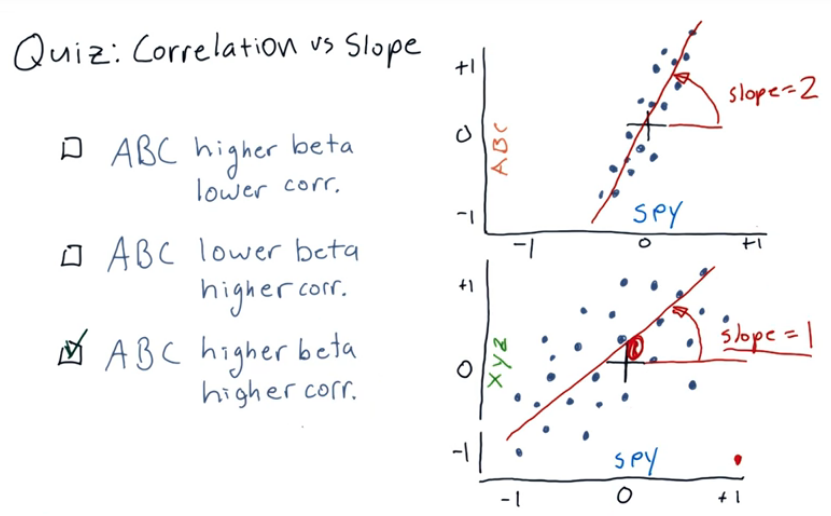
\includegraphics[scale=0.4]{fig/fig18}
\caption{$\beta$ vs correlation}
\end{figure}

%===================================================================================
\subsection{Sharpe ratio and other portfolio statistics}

\noindent
Portfolio: allocation fo funds to a set of stocks.

\subsubsection{Daily portfolio value} 

\begin{lstlisting}[language=Python, caption=]
start_val = 1000000
start_date = 2009-01-01
end_date = 2011-12-31
symbols = ["SPY", "XOM", "GOOG", "GLD"]
allocs = [0.4, 0.4, 0.1, 0.1]

"""" How do we calculate the total value of the portfolio day by day? """
normed = prices / prices[0]
alloced = normed * allocs
pos_vals = alloced * start_val
port_val = pos_vals * sum(axis = 1)
\end{lstlisting}

\begin{figure}[!ht]
\centering
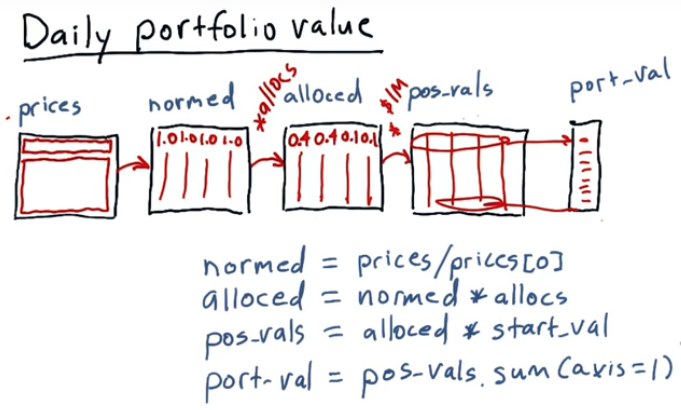
\includegraphics[scale=0.5]{fig/fig19}
\caption{Calculate portfolio value day by day}
\end{figure}

\subsubsection{Portfolio statistics}

\begin{lstlisting}[language=Python, caption=]
daily_rets = daily_rets[1:]
cum_ret = (port_val[-1] / port_val[0]) - 1
avg_daily_ret = daily_rets.mean()
std_daily_ret = daily_rets.std()
sharpe_ratio = ?
\end{lstlisting}

\begin{figure}[!ht]
\centering
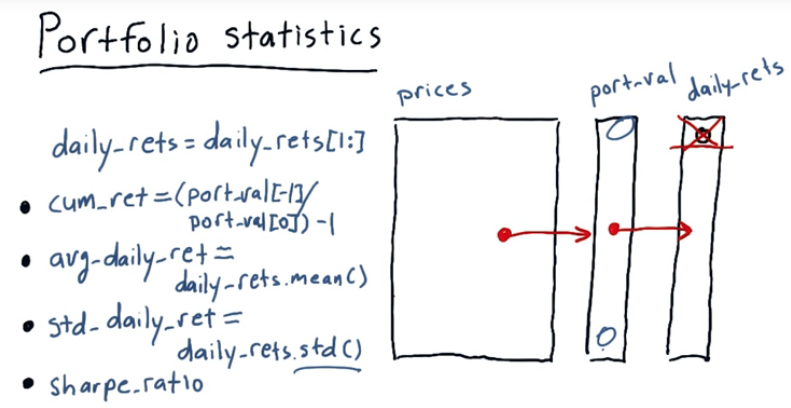
\includegraphics[scale=0.4]{fig/fig20}
\caption{Calculate portfolio value day by day}
\end{figure}

\subsubsection{Sharpe ratio}  

\noindent
(1) A metic that adjusts return for risk (risk adjusted return) \\
(2) All else being equal: lower risk is better; higher return is better \\
(3) SR also considers risk-free rate of return \\
\begin{equation}
S = \frac{R_p-R_f}{\sigma_p}
\end{equation}
$R_f$: portfolio return; $R_f$: risk-free rate of return; $\sigma_p$: std deviation of portfolio return (volatility). \\[8pt]
\noindent
Compute Sharpe ratio:
\begin{equation}
S = \frac{E[R_p-R_f]}{std[R_p-R_f]}
\end{equation}
Exact formulation; a forward looking measure (E[ ]). To calculate in reality, we need to look back at those values (taking mean):
\begin{equation}
S = \frac{\text{mean(daily\_rets - daily\_rf)}}{\text{std(daily\_rets - daily\_rf)}} = \frac{\text{mean(daily\_rets - daily\_rf)}}{\text{std(daily\_rets)}} 
\end{equation}
if assuming $\text{daily\_rf}$ being constant. \\[8pt]
\noindent 
What is risk-free rate?\\
(1) LIBOR (London Interbank Offer Rate) \\
(2) 3 mo Treasury bill \\
(3) 0 \\[8pt]
\noindent
Usually risk-free rate is not daily, but a percentage on an annual basis or a six month basis: \\
annual: 1.0 + 0.1 (at end of year) \\
daily: $^{252}\sqrt{1.0+0.1}-1$

\noindent
(1) SR can vary widely depending on how frequently you sample \\
(2) SR is an annual measure \\
(3) $SR_{annulized} = k * SR$ \\
(4) $k = \sqrt{\# \text{ of samples per year}}$ \\
daily $k=\sqrt{252}$, weekly $k=\sqrt{52}$, monthly $k=\sqrt{12}$. 

\begin{equation}
SR = \sqrt{252} * \frac{\text{mean(daily\_rets - daily\_rf)}}{\text{std(daily\_rets)}}
\end{equation}

%===================================================================================
\subsection{Optimizers: Building a parameterized model}

\subsubsection{What is an optimizer?} 

(1) Find minimum values of functions \\
(2) Build parameterized models based on data \\
(3) Refine allocations to stocks in portfolios 

\subsubsection{Minimizer in Python?} 

\begin{lstlisting}[language=Python, caption=]
import scipy.optimize as spo
result = spo.minimize(func, Xguess, method='SLSQP', options={'disp': True}) # result.X, result.func; def func(X)
result = spo.minimize(error, line_guess, args=(data,), method='SLSQP', options={'disp': True}) # def error(line, data)
result = spo.minimize(error, C_guess, args=(data,), method='SLSQP', options={'disp': True}) # def error(C, data)
\end{lstlisting}

\begin{lstlisting}[language=Python, caption=]
"""Fit a polynomial to a given set of data points using optimization."""
import pandas as pd
import matplotlib.pyplot as plt
import numpy as np
import scipy.optimize as spo

def error_poly(C, data):
    """Compute error between given polynomial and observed data.

    Parameters
    ----------
    C: numpy.poly1d object or equivalent array representing polynomial coefficients
    data: 2D array where each row is a point (x, y)

    Returns error as a single real value.
    """
    # Metric: Sum of squared Y-axis differences
    err = np.sum((data[:, 1] - np.polyval(C, data[:, 0])) ** 2)
    return err

def fit_poly(data, error_func, degree=4):
    """Fit a polynomial to given data, using supplied error function.

    Parameters
    ----------
    data: 2D array where each row is a point (x, y)
    error_func: function that computes the error between a polynomial and observed data

    Returns polynomial that minimizes the error function.
    """
    # Generate initial guess for polynomial model (all coeffs = 1)
    Cguess = np.poly1d(np.ones(degree + 1, dtype=np.float32))

    # Plot initial guess (optional)
    x = np.linspace(-5, 5, 21)
    plt.plot(x, np.polyval(Cguess, x), 'm--', linewidth=2.0, label="Initial guess")

    # Call optimizer to minimize error function
    result = spo.minimize(error_poly, Cguess, args=(data,), method='SLSQP', options={'disp': True})
    return np.poly1d(result.x)  # convert optimal result into a poly1d obeject and return

def test_run():
    # Define original polynomial
    Corig = np.poly1d([1.5, -10, -5, 60, 50])
    print("Original polynomial: {}*x^4 + {}*x^3 + {}*x^2 + {}*x + {}".format(Corig[4], Corig[3], Corig[2], Corig[1], Corig[0]))
    Xorig = np.linspace(-5, 5, 21)
    Yorig = np.polyval(Corig, Xorig)
    plt.plot(Xorig, Yorig, 'b--', linewidth=2.0, label="Original polynomial")

    # Generate noisy data points
    noise_sigma = 30.0
    noise = np.random.normal(0, noise_sigma, Yorig.shape)
    data = np.asarray([Xorig, Yorig + noise]).T  # Convert the input to an array, then transpose
    plt.plot(data[:, 0], data[:, 1], 'go', label="Data points")

    # Try to fit a polynomial to this data
    Cfit = fit_poly(data, error_poly)
    print("Fitted polynomial: {}*x^4 + {}*x^3 + {}*x^2 + {}*x + {}".format(Cfit[4], Cfit[3], Cfit[2], Cfit[1], Cfit[0]))
    plt.plot(data[:, 0], np.polyval(Cfit, data[:, 0]), 'r--', linewidth=2.0, label="Fitted polynomial")

    # Add a legend and show plot
    plt.legend()
    plt.show()

if __name__ == "__main__":
    test_run()
\end{lstlisting}

\subsubsection{Which functions would be hard to solve for a minimizer?} 
\begin{figure}[!ht]
\centering
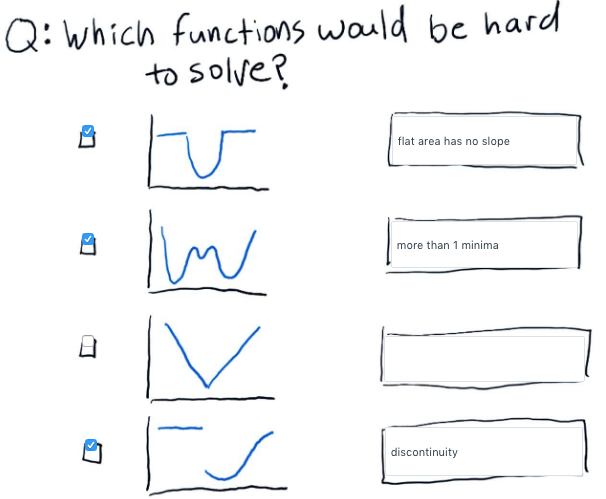
\includegraphics[scale=0.35]{fig/fig21}
\caption{Functions hard to solve for a minimizer.}
\end{figure}
 
\subsubsection{Convex problems} 
(1) Choose any two points, draw line \\
(2) Function is convex, if line is above graph 
\begin{figure}[!ht]
\centering
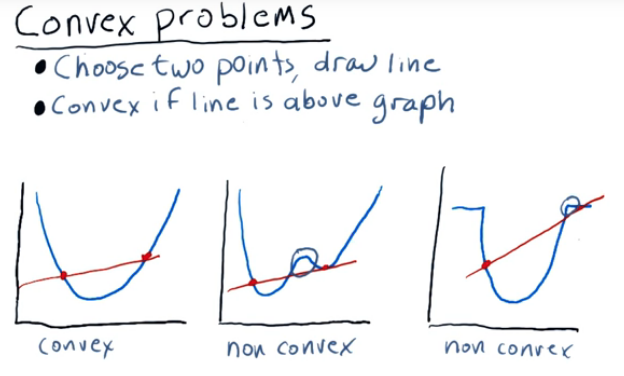
\includegraphics[scale=0.4]{fig/fig22}
\caption{Convex function?}
\end{figure}

\subsubsection{Building a parameterized model}       
\begin{figure}[!h]
\centering
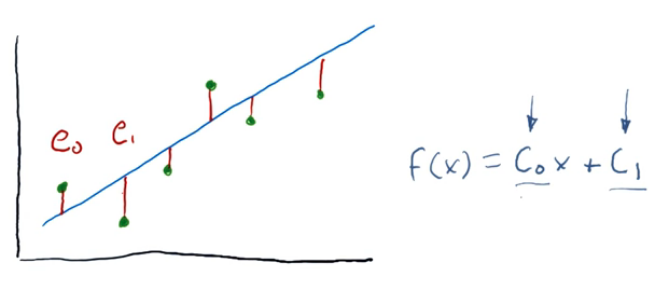
\includegraphics[scale=0.4]{fig/fig23}
\caption{Least squares}
\end{figure}

%===================================================================================
\subsection{Optimizers: Optimizers: How to optimize a portfolio}

\subsubsection{What are the metrics that can be used to optimize a portfolil?} 

(1) Maximum cumulative return \\
(2) Minimum volatility or risk \\
(3) Maximum risk adjusted return (Sharpe ratio) 

Cumulative return is the most trivial measure to use - simply investing all your money in the stock with maximum return (and none in others) would be your optimal portfolio, in this case. Hence, it is the easiest to solve for. But probably not the best for risk mitigation.

\subsubsection{Framing the problem: portfolio optimization} 

\noindent
Framing the problem: \\
(1) provide a function to minimize: f(x) = - Sharpe ratio \# x=allocations, to find minimum of f(x), thus maximum of Sharpe ratio \\
(2) provide initial guess for x \\
(3) call the optimizer \\ [5pt]
\noindent
Ranges and constraints: \\
(1) ranges: limits on values for x --$>$ [0, 1] \\
(2) constraints: properties of x that must be \q{true}, sum(x\_i) = 1

%%%%%%%%%%%%%%%%%%%%%%%%%%%%%%%%%%%%%%%%%%%%%%%%%%%%%%%
\section{Computational Investing}
%===================================================================================
\subsection{So you want to be a hedge fund manager?}

What is it you need to know, and what motivates you? It depends on what type of fund you manage and what your incentives are. Your motivation is probably compensation.And your compensation depends on the type of fund you manage and how well your fund performs.

\subsubsection{Types of funds}

% Table 1
\begin{table}[!ht]
\setstretch{1.5}
\centering

\begin{tabular}{l | l | l }
\multicolumn{2}{c}{} \\ [-10pt]
\hline
 ETF (Exchange-Tradeded Fund) & Mutual Fund & Hedge Fund \\
\hline
Buy/Sell like stocks & Buy/Sell at end of day & Buy/Sell by agreement \\
Baskets fo stocks & Quarterly disclosure & No disclosure \\
Transparent & Less transparent & Not transparent \\
\hline
\end{tabular}
\end{table}

\noindent
(1) \textcolor{red}{ETFs} are very much like stocks in the sense that you can buy and sell them. You can observe their prices intraday. You can trade them just like stocks on the stock exchange. 

They represent baskets of stocks. Sometimes they represent other instruments like bonds and so on. But it is very well-known and they publish what it is they are holding. Accordingly, ETFs are very transparent and they are very liquid. \\[5pt]
\noindent
(2) \textcolor{red}{Mutual funds} are somewhat similar to ETFs in the sense that they have a declared goal or mechanism. In other words, for instance, trying to track the S\&P 500 or some other such goal, but they are a little bit different. First of all, you can only buy or sell mutual funds at the end of the day. So at the end of the day they add up all the things they hold and compute a net asset value, and that is the value at which you can buy or sell shares of a mutual fund. 

They do not disclose exactly what they are holding except once every quarter, so they are accordingly less transparent. They are less transparent because since their last disclosure, you do not know exactly what they might have bought or sold. Still, they are somewhat transparent because they have stated goals and you know what they are trying to achieve, similar to, say, an ETF that might represent the S\&P 500. There are also mutual funds that represent large cap stocks like the S\&P 500. 

You have to go through some brokers, and you can't trade on your own. Typically, symbols of mutual funds have 5 letters (e.g., VTINX, FAGIX), and ETFs have 4 or 3 letters (e.g., DSUM, SPLV). \\[5pt]
\noindent
(3) \textcolor{red}{Hedge funds} are even less transparent than mutual funds. In fact, even to buy shares in a hedge fund, you have to enter an agreement that is secret, in the sense that you are not supposed to reveal the contents of that agreement. It is hard to exit a hedge fund. They usually require you to put your money in and leave it there for some number of months, sometimes years, and when you take it out, you can't necessarily take it out all at once. 

Hedge funds don't ever have to disclose what they're holding, not even to the investors in the hedge funds. Now, that might dissuade you from wanting, say, to invest in it if you don't know what they're holding. On the other hand, you know if they show you a good performance, you might want to invest. They will usually describe to clients what their strategy is and so on to encourage clients to invest. Accordingly, hedge funds are not transparent at all. 

Hedge funds typically have no more than 100 investors, whereas ETFS and mutual funds have thousands and maybe even millions of investors. \\[5pt]
\noindent
\textcolor{red}{Liquid} is the ease with which one can buy or sell shares in a particular holding. Stocks are extremely liquid. ETFs are liquid in the same way, in other words, you can go to a stock exchange, you can buy an ETF and sell an ETF. It's priced just like a stock, but when you buy it, you're buying shares of multiple stocks instead of just a single stock. But ETFs are liquid because they're easy to trade. They're also liquid in many cases because there's so much dollar value trading in them each day. If you look up an ETF on say Google Finance or Yahoo Finance, you can see how much volume is traded each day. And ETFs with higher volumes are even more liquid. 

\noindent
\textcolor{red}{Large cap}, where \q{cap} means capitalization, is how much is the company worth according to number of shares that are outstanding, times the price of the stock. So, some really huge cap stocks, say like Apple are worth many, many billions of dollars. There's also small cap stocks that are similarly, have lower value. 

\subsubsection{Incentives for fund managers}

\noindent
\textcolor{red}{Asset Under Management (AUM)}: the buzz word that is simply means how much money is being managed by the fund? For the three types of fund, part of the compensation is a percentage of the AUM. \\[5pt]
\noindent
Incentives: How are they compensated?
 
\noindent
(1) \textcolor{blue}{ETFs} managers are compensated according to an \q{expense ratio}, which is simply some percentage of AUM. Expenditure issues for ETFs are usually pretty low. They vary from as low as 0.01\% or, 1 bip as that might be called, to as high as 1\%. But one that's up to 1\% is fairly high and pretty unusual. 

\noindent
(2) \textcolor{blue}{Mutual funds} managers are also compensated using an expense ratio, which is somewhat higher than ETFs'. They range from a low of, typically, about 0.5\%, to somewhat that are very high, up to 3 \%. 

Why the difference? The way mutual funds managers manage funds requires much more skill. They have much more discretion than those who are managing ETFs. ETFs are usually tied to an index. As an example, a popular ETF, SPY is supposed to track the S\&P 500. And, all that an ETF manager has to do in that case is just make sure that they are holding all the stocks and the S\&P 500. Mutual funds, on the other hands, supposedly use more skill and therefore, they can charge a higher expense ratio both for the cost of research and also for their skill. 

\noindent
(3) \textcolor{blue}{Hedge funds} managers are compensated by following the old model called \q{Two and Twenty}, which means 2 or 2\% of AUM, plus 20\% of the profits. So as you can see, it's higher than both of these other methods. And most importantly, it includes this component relating to profits, that 20\%. 

However, the \q{Two and Twenty} structure has been assailed lately and it's very rare now to find a hedge fund that offers rates that high. They are much lower now, \q{One and Ten}, things like that. So the \q{Two and Twenty} was in the heyday of hedge funds in the 90s and early 2000s. Nowadays they are typically a little bit lower. There are some Star hedge funds that charge more. For instance, ASC Capital, which is no longer operating to the public anyways, they charge as much as 40\%, so it was \q{Four and Forty}. However, most hedge funds you find today will be somewhere between \q{Two and Twenty} or lower. 

% Table 2
\begin{table}[!ht]
\setstretch{1.5}
\centering
\begin{tabular}{l | l }
\multicolumn{1}{c}{} \\ [-10pt]
\hline
 ETFs & Expense Ratio, 0.01\% to 1.0\% \\
\hline
Mutual Funds & Expense Ratio, 0.5\% to 3.0\% \\
\hline
Hedge Funds & \q{Two and Twenty}\\
\hline
\end{tabular}
\end{table}

\noindent
The return of investors in these funds is based on how much the value of that fund increases and in most cases that increase is subject to what happens to the economy or what happens in the market. 

\subsubsection{How funds attract investors}

\noindent
\textbf{Who?} \\
(1) Individuals (i.e. extremely wealthy folks)\\
(2) Institutions (e.g., retirement funds like CalPERS in California, Harvard University Foundation) \\
(3) Funds of funds \\
Hedge funds typically can only have up to 100 investors. So they want each of those investments to be fairly large so that they can manage, of course, a significant amount of funds. So the individuals who invest in hedge funds are typically very wealth. \\
Funds of funds group together the funds of many individuals or institutions. For instance, you might be an individual that could invest in one hedge fund, buy you'd really like to get the advantage of investing in several funds. So you might allow your money to be collected by a manager of funds of funds. And that manager would gather together all these assets and pick carefully several hedge funds to invest that money in. \\[5pt]
\noindent
\textbf{Why?} \\
(1) Track record: Many institutional investors will want to see a good track record for at least 5 years before they'll invest in a particular fund. If you are a young whippersnapper hedge fund manager and you don't have 5 years, what you are gonna do? \\
(2) Simulation+story: What you do is simulate or back test your strategy, and investors will consider these simulations. But that simulation has to be backed by a very compelling story describing that strategy. In other words, you've gotta have a reason for why this method works and it needs to make sense. \\
(3) Good portfolio fit: Investors consider how your strategy fits within their portfolio. In other words, if your strategy is for large cap S\&P 500 stocks, and they've already got that covered with another fund, they might not consider you. However, if you, for instance, are looking at small cap growth stocks, and they don't yet have that part of their portfolio filled, they'll give you some more thoughts. 

\subsubsection{Hedge fund goals and metrics}

\noindent
\textbf{Goal} \\
(1) \textcolor{red}{Beat a benchmark} fund: Let's suppose, for instance, that you've got a strategy that looks at the stocks that are in the S\&P 500, there's 500 of them of course and you're especially smart at picking out the good ones. So you might build a hedge fund who's goal is to beat the S\&P 500 index as a benchmark because you're wise at selecting among all those, which stocks are going to outperform. Of course, the over all index has the good stocks and the bad stocks, so you're going to do better because you picked the specific good ones. 

An important component of the benchmark model is that many benchmarks, like the stock market as a whole, for which S\&P 500 is a good representative, go down. And it is of course natural that a portfolio consisted of stocks from this index might go down as well. So, even though both the index and the fund go down, you can outperform the index by doing down less. So, this kind of fund that is tagged against a benchmark can still meet performance goals if it goes down. So long as that index is going down more. \\
(2) \textcolor{red}{Absolute return} fund: Their goal is to bring positive return no matter what. These funds are usually long/short, which means they make positive bets in stocks they think are going to go up (long), and they make negative bets in stocks are going to go down (short). In any case their objective is to make slow gradual positive return no matter what. Often, these types of funds don't make the same percentage gains as the beat the benchmark fund, but they have very low draw downs. In other words, when the market takes a bit hit, they often don't. \\ [5pt]
\noindent
\textbf{Metrics} \\
(1) \textcolor{red}{Cumulative return} is a measure of, given the amount of funds I started with, how much more did I end up with after a certain amount of time? Cumulative return = (val[-1] / val[0]) - 1 \\
(2) \textcolor{red}{Volatility} is a measure of how rapidly and aggressively the portfolio goes up and down in value and of course lower volatility is better. Volatility = daily\_rets.std() \\
(3) \textcolor{red}{Reward/Risk} is a measure of the ratio of reward to risk. It's typically measured using Sharpe ratio. S.R. = risk adjusted reward = $\sqrt{252}$mean(daily\_rets - rf) / daily\_rets.std \\[5pt]
\noindent
Benchmark: The benchmark you choose should depend on the expertise you have. Let's suppose you're an expert in Eastern Europe. And you are great at picking stocks in emerging markets in Eastern Europe. You should select some benchmark that represents that similar kind of investing. There are indexes that represent emerging markets in Eastern Europe. There are also other funds whose values you might use as a benchmark. Or let's say you expertise is in banks. You might choose an index for the banking industry and show that you can beat that.

\subsubsection{The computing inside a hedge fund}

\noindent
Hedge funds are among the most computationally demanding environments. They have infrastructure requirements like huge databases, significant network connectivity, low latency and high bandwidth connectivity, real-time processing, and so on. The following is an example showing the typical kinds of computing that goes on inside a hedge fund. This isn't exactly the way all hedge funds work, but this is just to give you a taste for how many hedge funds work. Computing and computational capabilities are core here. \\[8pt]
\begin{figure}[!ht]
\centering
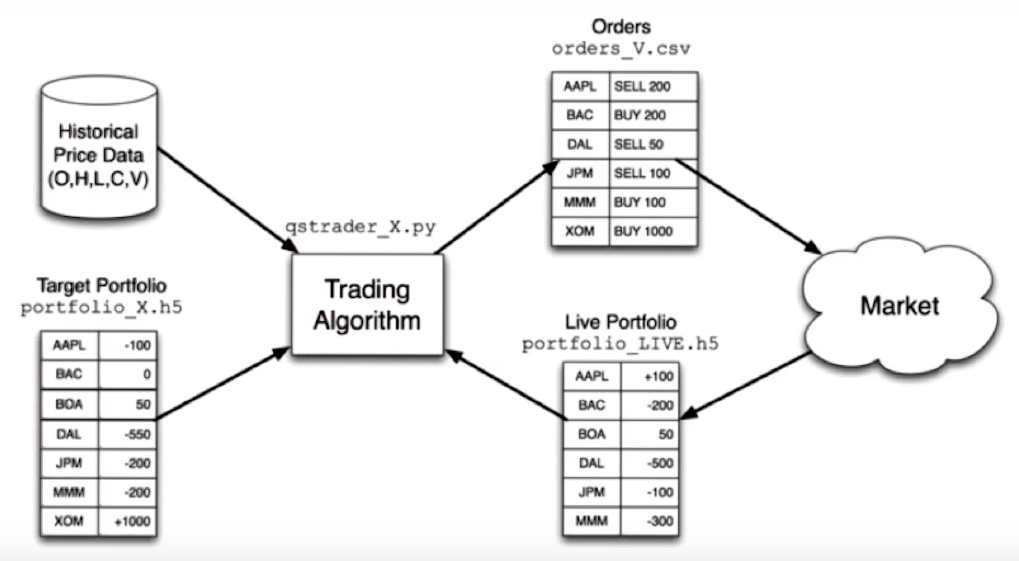
\includegraphics[scale=0.35]{fig/fig24}
\caption{Trading algorithm}
\end{figure}
\noindent
We work backwards from the market (Market) back towards the sort of back office of the hedge fund. The way things work are we have certain portfolio that is which stocks we have and whether we're in positive or negative positions with regard to them (Live Portfolio). The trading algorithm here is central (Trading Algorithm). It's interacting with the market, observing the live portfolio. And what it's trying to do is to get this live portfolio to match some target portfolio (Target Portfolio). So somewhere further back inside the hedge fund, we've decided what this target portfolio ought to look like. In other words, how many shares of Apple, how many shares of Delta Airlines we should have, and so on, and this trading algorithm is trying to get us there. So it's comparing target with live. And then to move this portfolio towards that target, it's issuing orders. So it sends orders like buy 200 shares of Apple to the market. Those orders get executed or not, and that updates the lie portfolio. 

One reason this kind of trading algorithm is important is you don't want to execute everything at once. In other words, suppose we wanted to take a very, very large position in Apple. If we were just to send an order, hey, buy me 10 million shares of Apple, that would affect us detrimentally in the sense that the price for Apple would probably rise. And we would not get a good execution. So this trading algorithm takes those sorts of things into consideration as it moves our live portfolio to be more close to the target portfolio. In fact, sometimes it takes days to enter a particular position. So this doesn't necessarily happen all at once. And there's many, many different types of trading algorithms that have been invented to solve these problems. \\[8pt]
\begin{figure}[!ht]
\centering
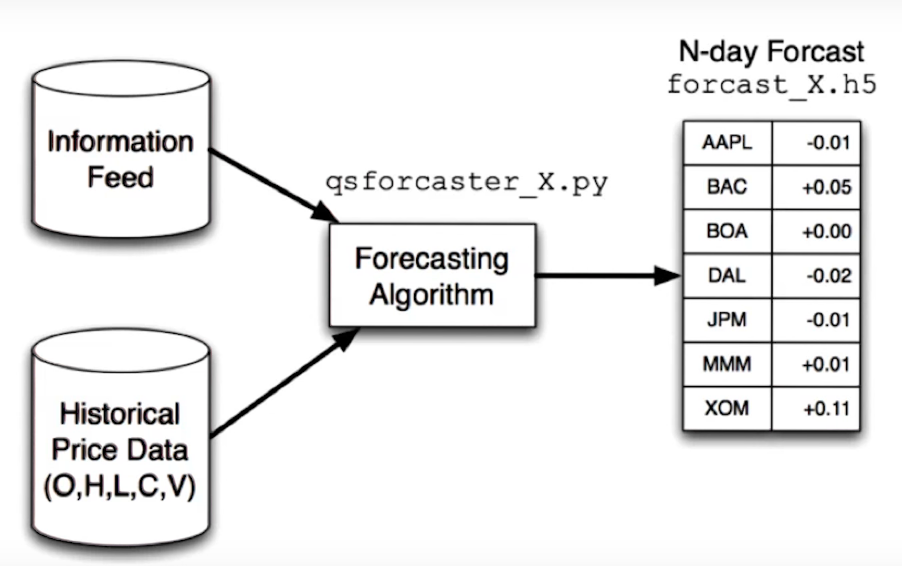
\includegraphics[scale=0.35]{fig/fig25}
\caption{Forecasting algorithm}
\end{figure}
\noindent
Now let's step one step back into the computing of the hedge fund, and look at how we arrive at this target portfolio. To arrive at the target portfolio, we need some data and computing that could go into computing the target portfolio. So from somewhere, machine learning perhaps, we have a forecast of what stock prices are going to be at some time into the future (N-day Forecast). And that can of course drive what our target portfolio ought to be for today. In other words, if we're forecasting that BAC is going to go up, this might represent that we think it's going to go up 5\%. We might want to increase our holdings in that. If we think that Apple, for instance, is going to go down, we might want to decrease our holdings. So this forecast informs this algorithm called a Portfolio Optimizer. That works to balance the risks and rewards for a balanced portfolio that considers volatility and correlation between different stocks and so on. 

Some other considerations that go into Portfolio Optimizer are historical data (open, high, low, close and volume). We can look at that historical data to inform how stocks are correlated or uncorrelated to one another. Also of critical importance is our current portfolio. It may be the case that if we're holding something, we don't want to exit it immediately because we'd be penalized by rapidly selling it. So this optimizer takes all this information into account to get to the target portfolio that our trading algorithm is working to drive us towards. \\ [8pt]
\begin{figure}[!ht]
\centering
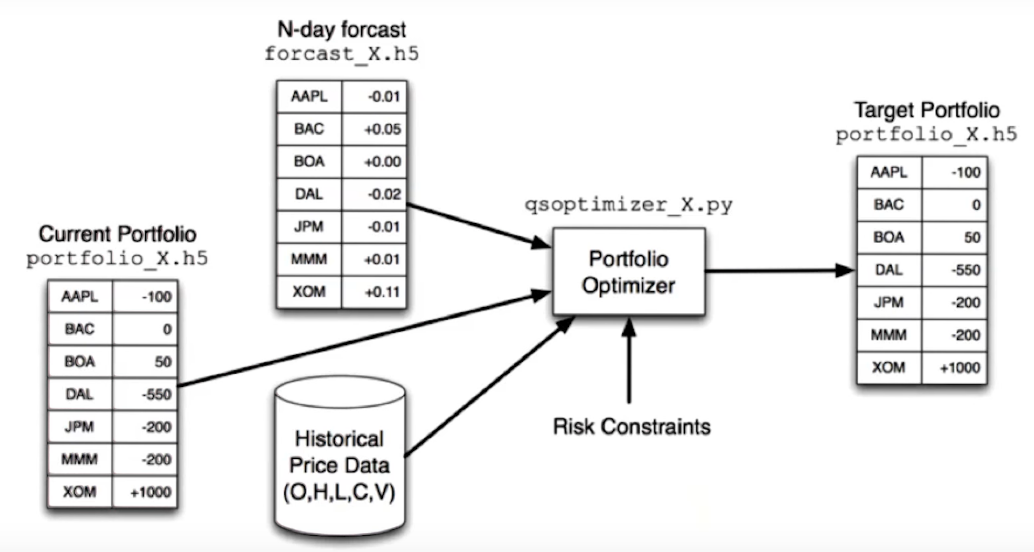
\includegraphics[scale=0.35]{fig/fig26}
\caption{Portfolio optimizer}
\end{figure}
\noindent
One more stop along our road at the computing infrastructure of a hedge fund is to look at how do we come up with this N-day forecast. N might be five days or ten days or whatever. Forecasting algorithm is very often in the form of a model, in fact, a machine learning based model. How do we get to this forecast? We've usually got some sort of proprietary information, historical data, and our forecaster crunches all that data to build a model and create a forecast. 

%===================================================================================
\subsection{Market mechanics}

When you trade stocks over the Internet, using a platform like E-trade, Interactive Brokers, or another online broker, what happens when you click buy?

\subsubsection{Order and order books}

The way that you build a portfolio, or buy stocks you hold in your portfolio, is by issuing orders. Usually you send those orders to a stock broker, and they take care of executing them for you. 

\noindent
\textbf{What is an order?} \\
(1) Buy or sell \\
(2) Symbol: An identifier for the stock or perhaps ETF that you want to buy or sell, for instance IBM or SPLV) \\
(3) \# shares \\
(4) Limit or Market: Limit means you don't want to do any worse than a certain price; for instance, suppose you're selling some stock. You might specify I don't want it to be sold below a particular price. Or if you're buying a stock, you might say, I don't want to pay more than a certain amount to get it. Market means you're willing to accept a good price but essentially whatever price the market is currently bearing) \\
(5) Price: If you're issuing a limit order, then you have to say what the corresponding price is. If it is a market order, you're not able to specify that price because essentially when you issue the market order you're saying I'll take whatever price comes back. \\ [8pt]
\noindent
Here are some examples: \\
\textcolor{blue}{BUY, IBM, 100, LIMIT, 99.95} \\
I wanna buy 100 shares of IBM at no more than \$99.95. \\
\textcolor{blue}{SELL, GOOG, 150, MARKET} \\
I wanna sell 150 shares of Google at Market price. \\[8pt]
\noindent
\textbf{The order book} \\
What happens when the order reaches the exchange?\\
A key construct at most exchanges is something called the order book. Each exchange keeps an order book for every stock that they buy or sell. Suppose the following order is the first that arrives at the New York Stock Exchange today:\\
\textcolor{red}{BUY, IBM, 100, LIMIT, 99.95} \\
In the order book: \\
\textcolor{blue}{BID\,\,99.95\,\,100} \\
Other may send in the same orders, then the number of shares will keep increase, say to 1000, then the order book keeps updating: \\
\textcolor{blue}{BID\,\,99.95\,\,100} \\
A new order comes in: \\
\textcolor{red}{SELL, IBM, 1000, LIMIT, 1000} \\
Updated order book is \\
\textcolor{blue}{ASK\,\,100.00\,\,1000} \\
\textcolor{blue}{BID\,\,99.95\,\,100} \\
Eventually, we have an order book 

% Table 2
\begin{table}[!ht]
\setstretch{1.5}
\centering
\begin{tabular}{l | r | r }
\multicolumn{2}{c}{} \\ [-10pt]
\hline
BID/ASK & PRICE & SIZE \\
\hline
ASK & 100.10 & 100 \\
\hline
ASK & 100.05 & 500 \\
\hline
ASK & 100.00 & 1000 \\
\hline
BID & 99.95 & 100 \\
\hline
BID & 99.90 & 50 \\
\hline
BID & 99.85 & 50 \\
\hline
\end{tabular}
\end{table}

\noindent
Suppose, now, a new order comes in:\\
\textcolor{red}{BUY, IBM, 100, MARKET} \\
The exchange looks at its order book and sees, yes, we have lots of shares for sale here. We have to give the clients the lowest price so we'll give that client 100 shares of these that are priced at \$100. After the transaction, our order book changes to 
% Table 2
\begin{table}[!ht]
\setstretch{1.5}
\centering
\begin{tabular}{l | r | r }
\multicolumn{2}{c}{} \\ [-10pt]
\hline
BID/ASK & PRICE & SIZE \\
\hline
ASK & 100.10 & 100 \\
\hline
ASK & 100.05 & 500 \\
\hline
ASK & 100.00 & 900 \\
\hline
BID & 99.95 & 100 \\
\hline
BID & 99.90 & 50 \\
\hline
BID & 99.85 & 50 \\
\hline
\end{tabular}
\end{table}

\textcolor{white}{.}\\[20pt]

\noindent
\textbf{How orders affect the order book?}
\begin{figure}[!ht]
\centering
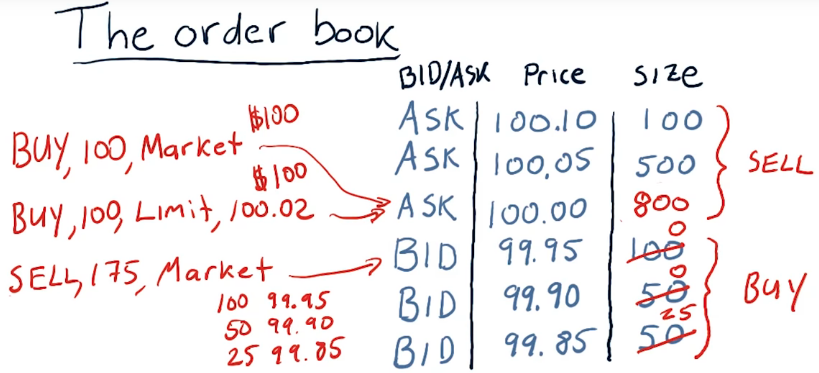
\includegraphics[scale=0.45]{fig/fig27}
\caption{How orders affect the order book?}
\end{figure}

\subsubsection{How orders get to the exchange?}

\noindent
\textbf{Scenario I:} \\
Your buy order goes over the internet to your broker. Your broker in turn is connected to several exchanges, and the broker determines where to route your order based on the information it knows about the exchanges. Your broker has a computer located at each exchange and it queries the computer to look at the order books at the changes and get the prices there. Query has added all the exchanges and your broker gathers and examines that information and based on that, routes your order to the exchange that has the best price. Let's say it's the New York Stock Exchange, your order enters the exchange, gets executed and the price comes back to your broker and forwarded back to you and you get a confirmation. 

It turns out that because this is happening constantly all the time, there's multiple brokers, hundreds of thousands, millions of people making orders that the order books at each of these exchanges tends to be pretty similar. In other words, the prices don't differ much between one or another and it's this sort of pressure that keeps prices the same across these different exchanges. 

\begin{figure}[!ht]
\centering
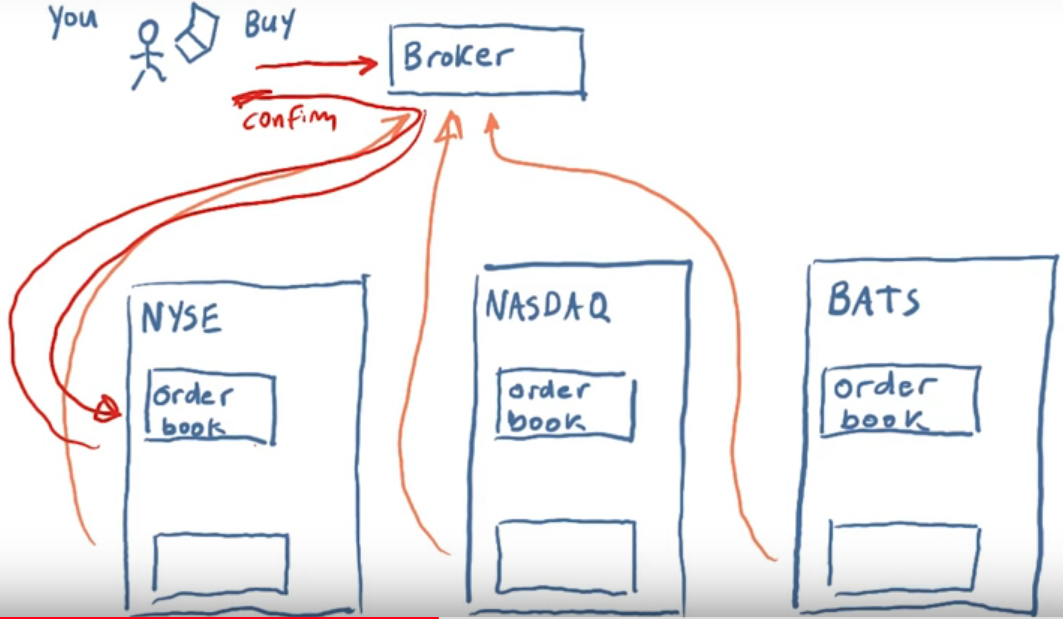
\includegraphics[scale=0.3]{fig/fig28}
\caption{Your order goes to the exchanges}
\end{figure}

\noindent
\textbf{Scenario II:} \\
Suppose there's another client of this same brokerage, Joe and that Joe wants to sell some stock. The brokerage can observe that I've got some clients who want to sell, some clients who want to buy. I can just make that exchange internally and I don't even need to go to the exchanges. This can be advantageous for the broker, because a broker doesn't have to pay now fees to the exchanges for this transaction to occur. 

However, according to the law, both the seller and the buyer have to get prices that are at least as good as they would've gotten if they had gone to an exchange. Eventually, at the end of the day, this transaction has to be registered with one the exchanges. Usually, it's recorded at the exchange, where that particular stock is homed. 

\begin{figure}[!ht]
\centering
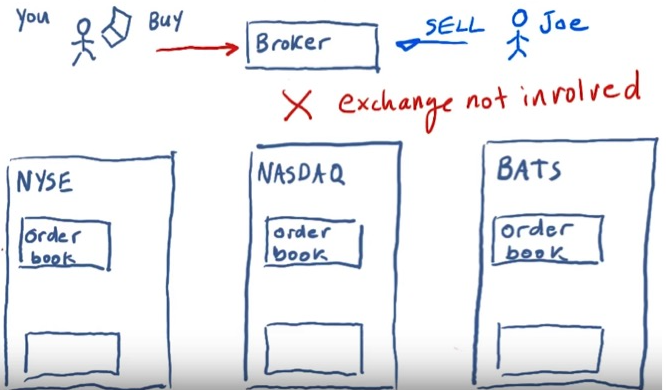
\includegraphics[scale=0.4]{fig/fig29}
\caption{One buy and one sell orders go to the same broker}
\end{figure}

\noindent
\textbf{Scenario III:} \\
There is one more entity called Dark Pool that acts as an intermediary between brokerages and exchanges. So the Dark Pool is looking at the order books of the various exchanges and they're often making predictions about which direction stocks are going to go. They actually pay the brokers for the privilege to look at the orders before they go to the exchanges.And if they see an advantageous trade, they'll go ahead and take it. So in this case, this cell might be routed through the Dark Pool from Broker 1 to Broker 2. 

And again, the transaction never makes it to the exchanges. In fact, these days, 80 to 90 \% of what they call retail traders orders never make it to the exchanges. They're either executed internally within a brokerage or filled using a Dark Pool. The brokerages in the Dark Pools argue that, that's just fine, because both partners in this transaction are getting prices at least as good as they would get at the exchanges on the order books. But they're saving money because they don't have to pay the exchange fees. 

\begin{figure}[!ht]
\centering
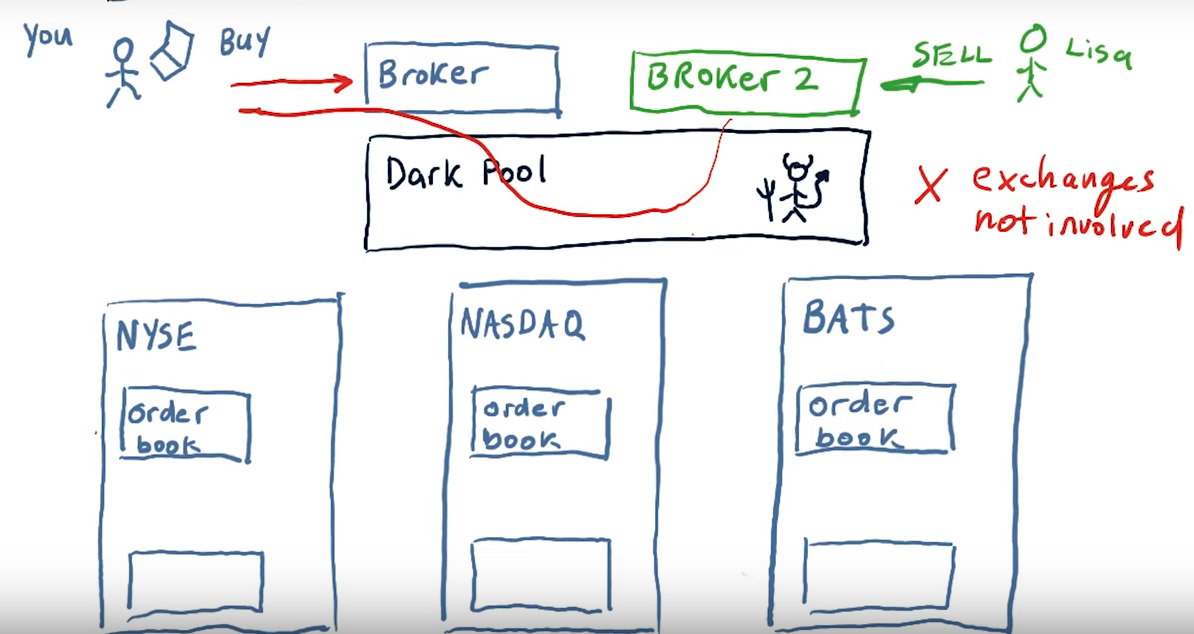
\includegraphics[scale=0.3]{fig/fig30}
\caption{Dark Pool acts as an intermediary between brokerages and exchanges.}
\end{figure}

\subsubsection{How hedge funds exploit market mechanism/inefficiencies?}

\noindent
You enter a buy order. Your order travels all across the country, because you use E-trade, it stops in Atlanta, and then it hops to New York City. Suppose our hedge fund has a colocated computer. And it's observing the order book as well. Here is the advantage that the colocated hedge fund has: its computer is located maybe 100 meters away from the main exchange computer that holds the order book, so that 100 meters amounts to 0.3 microseconds in terms of how long it takes information about the order book to reach that hedge fund computer. You, on the other hand, are located at least 2500 miles away. And that means when this order book changes, it takes 12 milliseconds at least for that information to get to you and 12 milliseconds at least for your order to reach the exchange. 

Here is how the \textcolor{red}{order book exploit} works. The hedge fund is continually observing the order book, and it takes only 0.3 microseconds for it to do that. Based on what it sees at the order book, it thinks the price is going to go up. The hedge fund buys some of that stock based on what it sees. You are thinking the same thing, so you've entered buy. And your order starts making its way across the country. While your order is coming across the country, indeed, the price is going up, because other orders are coming in from other places. Eventually, your order makes it to the New York Stock Exchange and is executed there. And, in fact, the hedge fund sells it to you. Over this few fractions of a second, the hedge fund has bought some stock, watched it go up and sold it. It might have held this 100 shares of stock for only a few milliseconds and made a profit. And the hedge fund is exploiting essentially all these people remotely located around the country observing the order book, essentially late sending in orders that it can take advantage of because it can act much earlier before those orders from around the country arrive. \\ [8pt]
\begin{figure}[!ht]
\centering
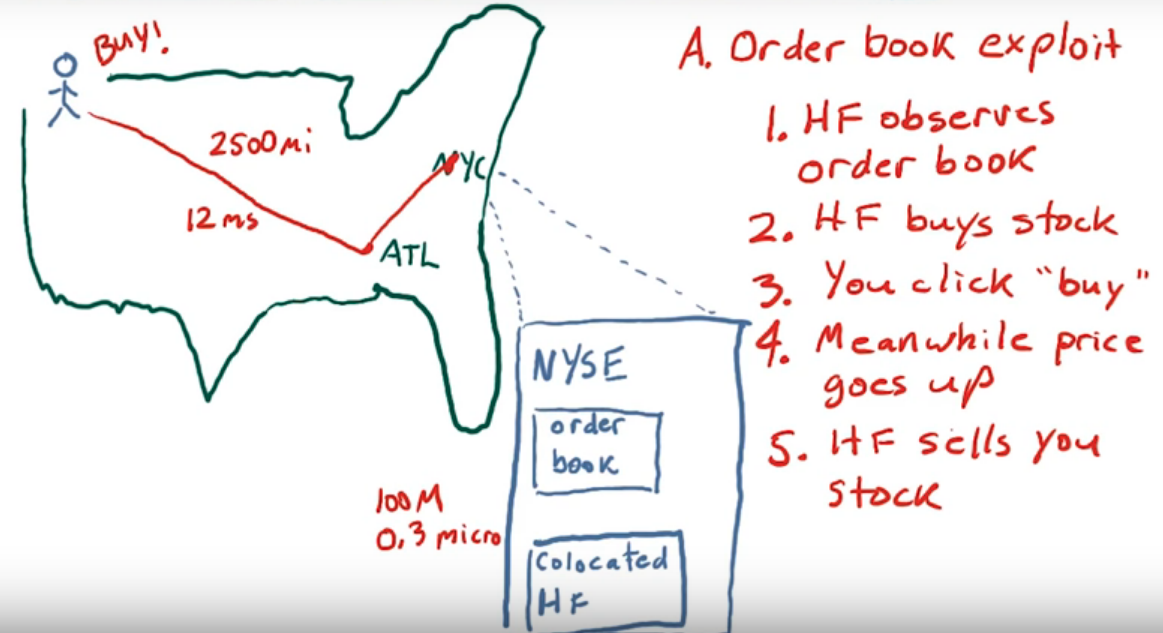
\includegraphics[scale=0.3]{fig/fig31}
\caption{Order book exploit}
\end{figure}
\noindent
There are certainly many sorts of ways to exploit market mechanics. Here is one more, I call this one the \textcolor{red}{geographic arbitrage} exploit. Suppose we have exchanges located some distance away and because they're located distantly prices may drift a little bit up or down. A hedge fund might place their own servers at each of these Exchanges and connect them with an ultra high speed dedicated connection. And they are observing the order book, the prices at both these locations all the time and comparing notes. Let's suppose a difference emerges that in New York the price is a little bit lower, in London price is a little bit higher. The fund will immediately buy in New York, and sell in London. They are not necessarily even transferring those same shares. They might buy some set of shares in New York City, and sell a different set in London. But they are getting that difference in price advantage immediately. Because hedge funds are monitoring the prices all over the world, these sorts of differences rarely arise and when they do it's just by fractions of a cent. But those differences do arise because there are inefficiencies in the markets and there are hedge funds there to pick those pennies up off the ground. 

\begin{figure}[!ht]
\centering
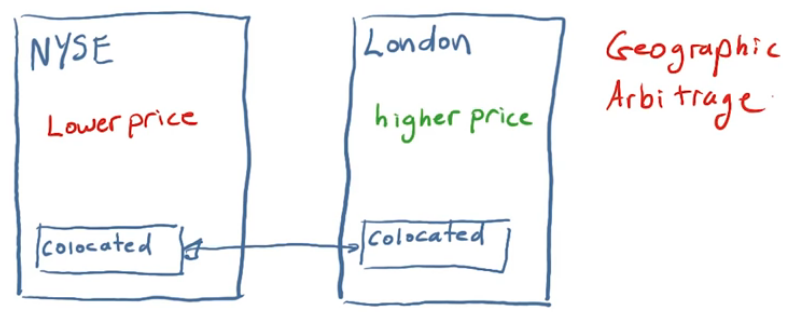
\includegraphics[scale=0.45]{fig/fig32}
\caption{Geographic arbitrage exploit}
\end{figure}

\subsubsection{Additional order types}

\noindent
Exchanges\\
(1) Buy Sell \\
(2) Market Limit \\
Exchanges only execute these types of orders, and don't execute other types of order. How do those other types of orders come into being? They are implemented by your broker. \\
(1) Stop loss \\
(2) Stop gain \\
(3) Trailing stop \\
(4) Selling short \\
You enter this order type, and your broker holds that order and watches the market until the conditions that you specified are met and then when those conditions are met, the broker sends your order to the market accordingly. \\[8pt]
\noindent
\textcolor{red}{Stop loss} is a kind of order where you say when the stock drops to a certain price, I want you to sell it. \\
\textcolor{red}{Stop gain}, similarly, is when the stock reaches a certain higher price, I want you to sell it. \\
\textcolor{red}{Trailing stop} is a combination of stop loss but also an automatically changing value for when the criteria is met. For instance, you might have this trailing stop remain \$0.10 behind the price. So as the price goes up, the value at which you would want to sell the stock goes up along with the price, but when it drops down below, then that stop loss is triggered. \\
\textcolor{red}{Selling short} is probably the most import and most impactful kind of order the brokers implement for you. Selling short allows you to take a negative position on a stock, in other words, you sell a stock if you believe its price is going to go down. Keep in mind here we're selling stock we don't even own. How is it possible? It's possible because the broker facilitates it for you.   

\subsubsection{Short selling}

You want to take a short position in IBM, and IBM is currently selling at \$100, which is the current market price. Joe holds 100 shares of IBM. He likes IBM, he wants to hold onto it. But he's willing to lend you those shares of IBM. In fact, Joe's broker will take care of that for him. He may not even know that he's lending you the shares. Let's suppose Lisa thinks that IBM is going to go up and she wants to buy IBM. So you want to sell IBM short; you don't own any shares of it. Lisa wants to buy IBM; she thinks it's going to go up. So here's what happens. You borrow that 100 shares from Joe. Now that you have those shares, you can turn around and sell them to Lisa. And in exchange for those 100 shares that you gave Lisa, she gives you 100 times \$100, or \$10,000. The result of this transaction, after everything settles, is you have \$10,000 in your account but you owe Joe 100 shares of stock. And of course, Lisa has 100 shares of stock and so on. Now the problem sort of arises here that Joe may decide he wants his 100 shares back. What you'll have to do is go buy them from someone and then give them back to Joe. 

\begin{figure}[!ht]
\centering
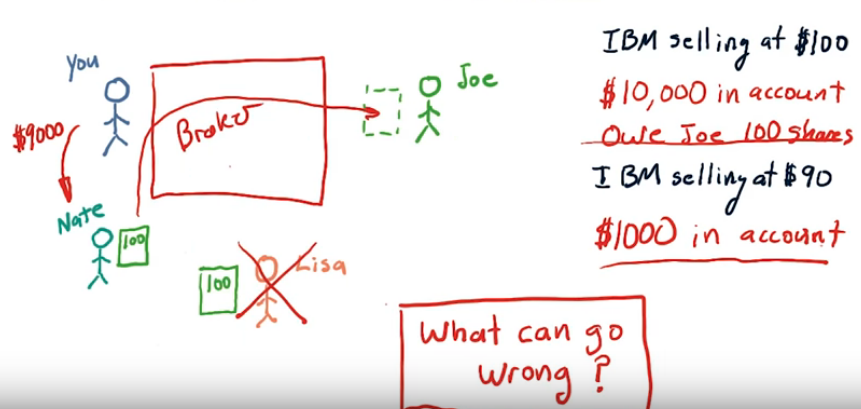
\includegraphics[scale=0.45]{fig/fig33}
\caption{Short selling}
\end{figure}

Since then IBM has dropped in price and now it's selling at \$90. You can make a profit of that and you want to go ahead and exit.You approach Lisa to buy the 100 shares back; but Lisa wants to keep IBM. But there is somebody out of there, Nate, who's got 100 shares and is willing to sell them. So you buy 100 shares from Nate and give them back to Joe. So your obligation to Joe is now completed. IBM is selling at \$90, so you had to give Joe \$9000. But you had \$10,000, so the net result after everything is said and done is you've got a \$1000. 

In reality, you don't have to make these personal agreements with those people, your broker makes all that happen. What can go wrong? What if IBM went up to \$150 per share, and now you want to exit your position? You lose money.

%===================================================================================
\subsection{What is a company worth?}

\subsubsection{Why company value matters?}

\begin{figure}[!ht]
\centering
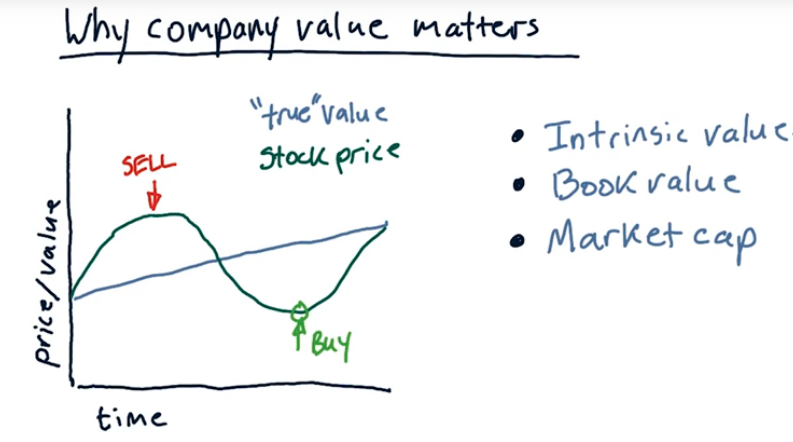
\includegraphics[scale=0.45]{fig/fig34}
\caption{Why company value matters?}
\end{figure}

In general, the value of a company goes up monotonically. Let's assume it is the true value (intrinsic? book?) of the company. The true value is distinct and different from the value estimated by the market. In other words, what price the stock market says, it's worth? Many trading strategies focus on identifying situations where the current stock price is different from the true value. So in other words, if the stock price goes up a lot, but we know the actual company is only worth a certain amount. When it goes high, that might be a selling opportunity. Similarly, if we see the price really low compared to what the company is worth, that could represent a buying opportunity. 

\subsubsection{Compute company value}

\textcolor{red}{Intrinsic value}: Only considering dividends, how much value is the company expected to generate over its lifetime? In other words, it is based on the value of the company as estimated by future dividends. Many companies pay each year or each quarter a dividend. So it's a cash payment if you own a stock you get a certain amount of dividend. Essentially, it is the value of all the future dividends (all the way to infinity) the company is going to pay.

\begin{figure}[!ht]
\centering
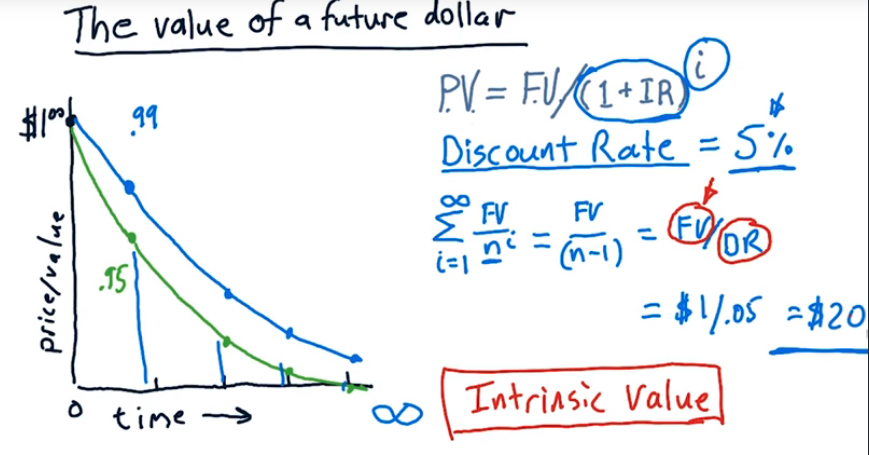
\includegraphics[scale=0.4]{fig/fig35}
\caption{Intrinsic value}
\end{figure}

\textcolor{blue}{Discount rate}: It is higher if you trust the company less or you think it's more risky; it is lower if it's more certain to pay you that dividend every year. 

Interest Rate and Discount Rate are terms that refer to essentially the same quantity, but are used to distinguish two slightly different use cases: (1) Interest Rate is used with a given Present Value, to figure out what the Future Value would be. (2) Discount Rate is used when we have a known or desired Future Value, and want to compute the corresponding Present Value.\\[8pt]
\noindent
\textcolor{red}{Book value}: What is the company worth, \q{on the books}? That is, if the company owner(s) sold all the assets (that can be sold) and paid off all dues, how much money would they make/lose? Intangible assets (e.g. patents, brand name) are not considered. \\[8pt]
\begin{figure}[!ht]
\centering
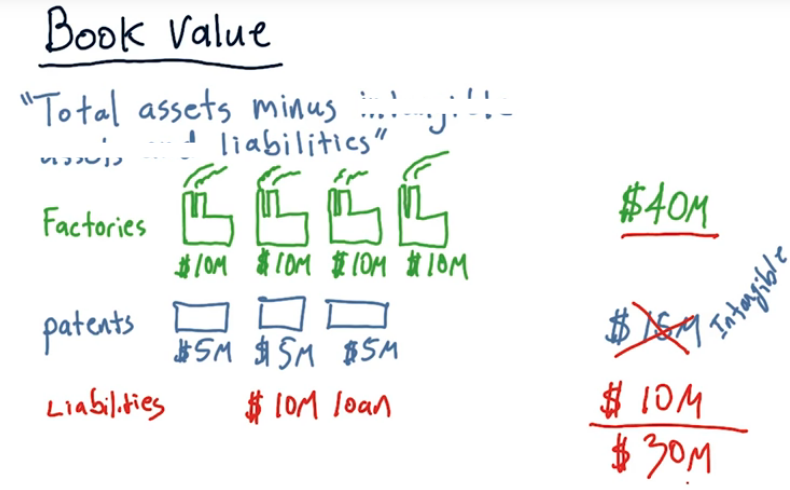
\includegraphics[scale=0.4]{fig/fig36}
\caption{Book value}
\end{figure}
\textcolor{red}{Market capitalization}: What is the company worth on the market? In other words, how much money will you have to pay to buy the entire company.
\begin{equation}
\text{Market cap} = \text{\# shares} * \text{price} \nonumber
\end{equation}

\subsubsection{Would you buy this stock?}

Many stock trading strategies look for deviations between intrinsic value and market cap. If intrinsic value drops significantly and the stock price is high, it may be worthwhile to short the stock. Or if say dividends are going up and the market capitalization is low, it might be an opportunity to buy the stock. Similarly, book value provides a sort of lowest price, when stock price begins to approach book value, you can pretty much assume that the price is not going to go below book value, or not much below it, because if it does, a predatory buyer would buy the whole company, and break it up for parts. So stock rarely goes below the book value of the company!

A company has market capitalization \$75M, book value \$80M, and intrinsic value \$20M.

Ignoring the intrinsic value, if you buy the entire company off the market (for \$75M) and immediately sell it for its book value (\$80M), you have a \$5M profit right there! Even if you are buying some stocks (instead of the whole company), the stock price is expected to increase (as it is currently undervalued).

%===================================================================================
\subsection{The Capital Assets Pricing Model}

This section covers the most significant ideas affecting finance in the last century. It explains how the market impacts individual stock prices. And it also provides a mathematical framework for hedge fund investing. It's called the Capital Asset Pricing Model or CAPM for short. It was developed by a number of researchers independently in the 1960s. William Sharpe, Harry Markowitz and Merton Miller jointly received the Nobel Prize for this contribution in 1990. The CAPM led to the development of index funds and the belief that you can't beat the market. 

\subsubsection{Portfolio and market portfolio}

A portfolio is a weighted set of asset. \\
(1) $w_i$: portion of funds in asset i; \\
(2) $\sum{|w_i|}=1.0$. \\
For leveraged portfolio, this can be greater than 1; we allow short selling, so $w_i$ can be negative. \\[8pt]
\noindent
When someone refers to the Market, what they're usually referring to is an index that broadly covers a large set of stocks. In the US, best example of that is the S\&P 500. It represents the 500 largest companies that are traded on exchanges, and that index changes each day according to the prices of all of its components. 

\begin{figure}[!ht]
\centering
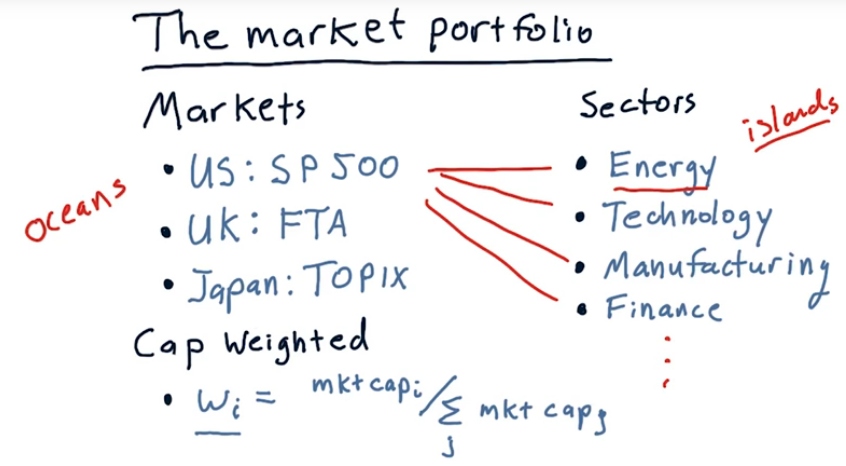
\includegraphics[scale=0.4]{fig/fig37}
\caption{Market portfolio}
\end{figure}

The index represents many many stocks, and the market portfolio is a combination of those stocks in a certain weighting. Most of the important indexes are what we call Cap Weighted. It means the individual weight of each stock in the portfolio is set according to that stock's market cap. In the US, markets are divided into 10 sectors. One thing to keep in mind is some stocks have surprisingly large weightings. For instance, Apple and Exxon each are about 5\% of the S\&P 500. So those two stocks have a strong effect on what happens to this index. There are smaller stocks that comprise only a tenth of a percent of the overall effect on the market. 

\subsubsection{The CAPM equation}

\begin{figure}[!ht]
\centering
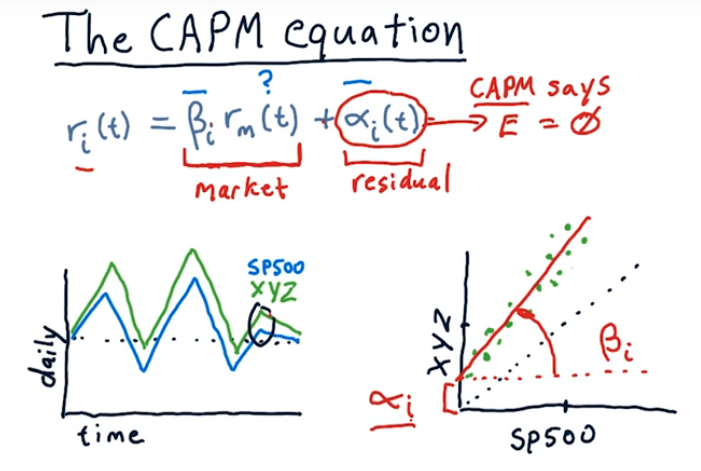
\includegraphics[scale=0.4]{fig/fig38}
\caption{The CAPM equation}
\end{figure}

\noindent
The CAPM equation says that the return of an individual stock ($r_i(t)$) on a particular day $t$ is equal to $\beta_i$ times the return on the market ($r_m(t)$, S\&P 500 in the US) plus $\alpha_i(t)$ of that particular stock on that day. And this particular stock, $i$, is one of the stocks in the S\&P 500.

The CAPM is asserting is that a significant portion of the return for a particular stock is due to the market. In other words, the market moving up or down strongly affects the change in price on every individual stock. The extent to which the market affects a particular stock is encapsulated in this $\beta$. Every stock has its individual $\beta_i$ that specifies how much it's affected. Many stocks have $\beta$ near 1, which means when the market goes up or down 1\%, that stock goes up or down 1\%. The other component, $\alpha$, is called the residual. 

An important part of CAPM is that the expectation for $\alpha$ is 0 ($\text{E}[\alpha_i(t)]=0$). Essentially this is a random variable with an expected value of 0. 

$\beta$ and $\alpha$ come from daily returns, essentially how the daily returns for a particular stock relate to the daily returns of the market. In the graph, the XYZ stock is more reactive, in other words, if S\&P 500 goes up a little, this stock goes up more. On average, it tends to have a higher return each day. We convert the daily returns plot to a scatter plot and fit a line to it. $\beta$ is the slope and $\alpha$ is the y-axis intercept of that line. This is an \q{after-the-fact} calculation. Just because historically a particular stock, looking back at time gave you a particular $\alpha$, you shouldn't necessarily expect that in the future. Again, CAPM says you should expect $\text{E}[\alpha_i(t)]=0$. In reality though, it's not always 0. 

\subsubsection{CAPM vs active management}

\textbf{Passive investing vs active investing} 

\noindent
Passive: buy index portfolio (e.g. S\&P 500) and hold \\
Active: pick stocks (i.e. pick individual stocks, overweights for some stocks and lower weights for other stocks)

The active portfolio manager's portfolio differs from the market portfolio by selecting different weights on different stocks. Both active and passive managers agree with the part, $\beta_ir_m(t)$---how the stock moves each day is most significantly influenced by the market, and the amount that it moves is strongly related to $\beta$. Where they differ is with regard to their treatment of $\alpha$: CAPM says $\alpha$ is random and you can't predict it, and $E[\alpha]=0$; active managers believe they can predict $\alpha$. 

\begin{equation}
r_i(t) = \beta_ir_m(t) + \alpha_i(t)
\end{equation}

Remember this $\alpha$ is market-relative. Active managers believe they can compare two stocks and say I think this stock is going to go up relative to the market. Or, I think this other stock is going to go down relative to the market. They might not be exactly right on every single pick. But they believe on average they're better than just flipping a coin. If you believe what active managers say, you can use this information and perhaps machine learning to find stocks that have either positive or negative $\alpha$. And you can use that information to select your stock picks. 

Anyways, if you believe the capital assets pricing model, in other words, this $\alpha$ is fully random, then you should be a passive investor, just buy an index and hold it. If you believe active managers, that they can find $\alpha$, then you should consider being an active investor. 

\subsubsection{CAPM for portfolios}

CAPM says that for a portfolio return, we have
\begin{equation}
r_p(t) = \sum_iw_i(\beta_ir_m(t) + \alpha_i(t)) = \beta_pr_m(t) + \alpha_p(t)
\end{equation}
where $\beta_p = \sum_iw_i\beta_i$. Since CAPM says that all of these $\alpha_i(t)$ are on average going to be zero, so we don't need bother necessarily adding them up, we can just approximate it by an overall portfolio $\alpha_p$.

However, the active portfolio managers believe they can find value in $\alpha_p$ and it needs to be broken out individually. 
\begin{equation}
r_p(t) =  \beta_pr_m(t) + \sum_i{w_i\alpha_i(t)}
\end{equation}

\subsubsection{Implications of CAPM}

CAPM says $r_p = \beta_pr_m + \alpha_p$. It has two implications: (1) expected value of $\alpha$ is 0; (2) the only way to beat market is choose a positive $\beta$ when the market is going up and a negative $\beta$ when the market is going down (choose high $\beta$ in up markets, choose low $\beta$ in down markets). 

\begin{figure}[!ht]
\centering
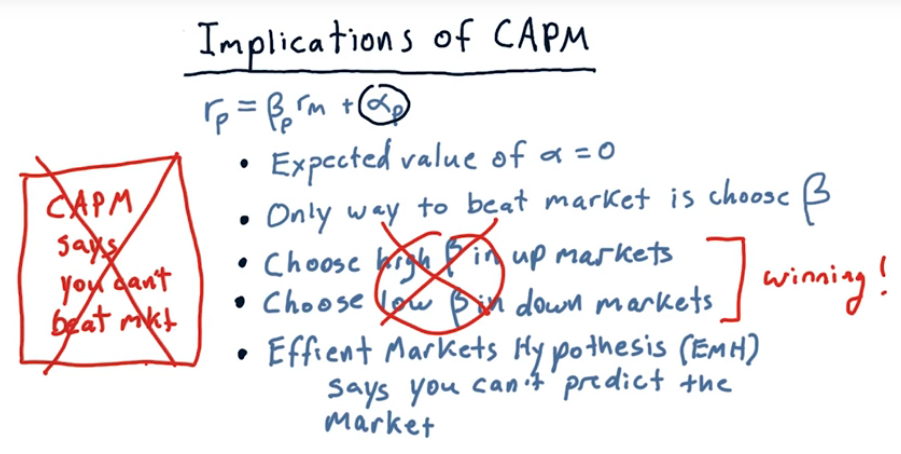
\includegraphics[scale=0.45]{fig/fig39}
\caption{Implications of CAPM}
\end{figure}

The only problem with that is the efficient markets hypothesis. Efficient Markets Hypothesis (EMH) says you can't predict the market. Therefore, you can't beat the market. Can you?

\subsubsection{Arbitrage pricing theory}

In CAPM, $r_i = \beta_ir_m + \alpha_i$, we have the single $\beta$ that represents a particular stock's relationship to the market. Maybe really we ought to have multiple $\beta$s. Stephen Ross (1976) argues that a particular stock might have exposure to different aspects of the market. So, the stock might have some exposure to finance, so we could compute the component of return due to finance via the $\beta$ with regard to finance ($\beta_{iF}$) and the return for finance that day ($r_F$). So we could compute for each stock, for each sector, and individual $\beta$. So the assertion is that by breaking out the $\beta$s into these different factors, we can get more accurate forecast of what the return's going to look like. 

\begin{figure}[!ht]
\centering
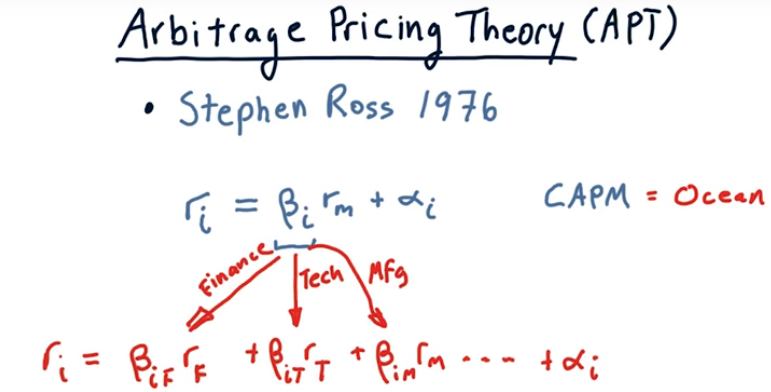
\includegraphics[scale=0.4]{fig/fig40}
\caption{Arbitrage pricing theory}
\end{figure}

%===================================================================================
\subsection{How hedge funds use the CAPM}

A typical hedge fund develops methods to find stocks they think will perform well. The informational edge that they're seeking is usually market relative, meaning they're looking for stocks that will go up more than the market if the market goes up, your stock will go down less than the market if the market goes down. If this information they have is reliable, they can take advantage of the CAPM to virtually guarantee positive return. 

\subsubsection{Two stocks scenario}

\begin{figure}[!ht]
\centering
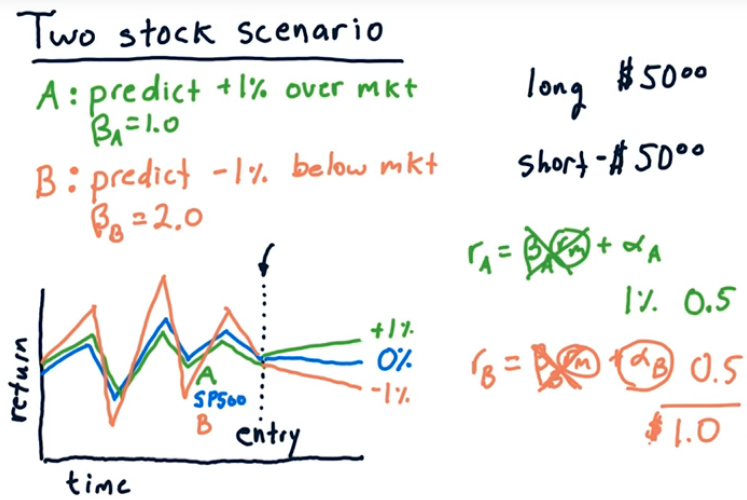
\includegraphics[scale=0.4]{fig/fig41}
\caption{Two stocks scenario: $r_m=0\%$}
\end{figure}

\begin{figure}[!ht]
\centering
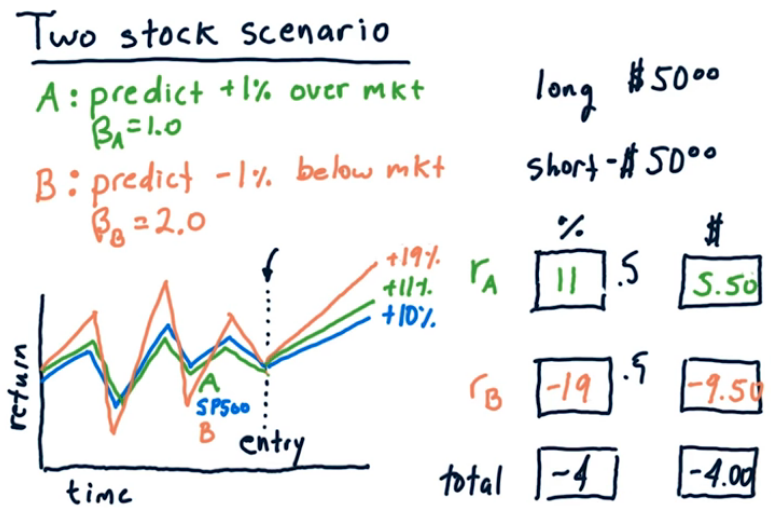
\includegraphics[scale=0.4]{fig/fig42}
\caption{Two stocks scenario: $r_m=10\%$}
\end{figure}

\begin{figure}[!ht]
\centering
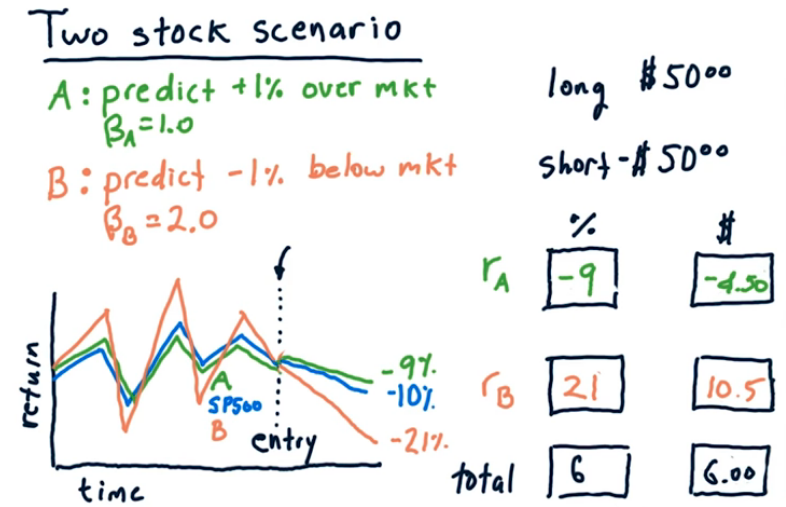
\includegraphics[scale=0.4]{fig/fig43}
\caption{Two stocks scenario: $r_m=-10\%$}
\end{figure}

The take away is even if we have perfect $\alpha$ and perfect $\beta$, if we are not careful about how we allocate our money, we can still lose. To fix this, we can use CAPM. 

\subsubsection{Two stock CAPM math}

We can calculate the portfolio return by using the CAPM equation. We have some information about the stocks ($\alpha_p$) that lead us to believe one would go up 1\% over the market, another would go down 1\% over the market. On the other hand, we don't really have any knowledge about what's going to happen for the market over all. So we have no control over the component related to $\beta$. Is there some way can we remove this component by setting it to 0? If we can do that, then we essentially remove market risk from our portfolio. And we preserve this $\alpha_p=1\%$, no matter how the market goes.

We need to add a lot of caveats here. These $\beta$s aren't necessarily fully guaranteed to continue into the future, and these $\alpha$s aren't guaranteed, either. This allocation is not a guaranteed thing by any means, but it's a way to use long/short investing to reduce exposure to the market overall and to focus on those $\alpha$ components where we do have information.  

\begin{figure}[!ht]
\centering
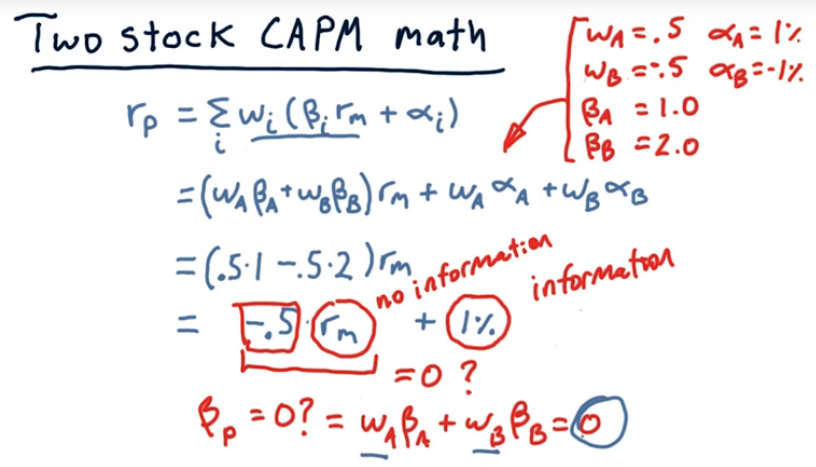
\includegraphics[scale=0.4]{fig/fig44}
\caption{Two stocks CAPM equation}
\end{figure}

%===================================================================================
\subsection{Technical analysis}

\subsubsection{Technical versus fundamental analysis}

There are two broad categories of approaches to use for choosing stocks to buy or sell. They are based on fundamental analysis and technical analysis. \textcolor{red}{Fundamental analysis} involves looking at aspects of a company in order to estimate its value. Fundamental investors typically look for situations where the price of a company is below its value. Another CAPM is based on \textcolor{red}{technical analysis}. Technicians don't care about the value of a company. Instead, they look for patterns or trends in a stock's price. 

\subsubsection{Characteristics of technical analysis}

\textbf{What it is} \\
(1) historical price and volume only\\
(2) compute statistics called indicators \\
(3) indicators are heuristics 

Technical analysis looks at historical price and volume only. That's as opposed to fundamental analysis that looks at fundamental factors, like earnings, dividends, cash flows, book value, and so on. We look back at historical price and volume to compute statistics on this time series, and these statistics are called indicators. Indicators are heuristics that may hint at a buy or sell opportunity. 

There is significant criticism of the technical approach. People think it's not an appropriate method for investing, because it's not considering the value of the companies. Instead, maybe you could think about it as a trading approach as opposed to an investing approach. \\[8pt]
\noindent
\textbf{Why it might work} \\
(1) there is information in price \\
(2) heuristics work 

Information in price change reflects sentiments of buyers and sellers, and especially if we see that the price for a particular stock is moving in a different direction than the overall market, that might be a hint that there's something going on. Additionally, we know that in other domains of artificial intelligence, heuristics can work, and they work frequently. 

Even though it's controversial, there are reasons to believe technical analysis can work. 

\subsubsection{When is technical analysis effective}

Rules of thumb: \\
(1) Individual indicators weak \\
(2) Combinations stronger \\
(3) Look for contrasts (stock vs market) \\
(4) Shorter time periods

Individual indicators, by themselves, are weakly predictive. Back in the 80's and 90's when some of these indicators were created, they had stronger value. But since that time, more and more people have been trading according to them, and essentially the more people who are following a particular approach, the less value is realized by any person by themselves. 

However, combining multiple indicators adds value. Combinations of 3 to 5 different indicators, in a machine learning context, provide a much stronger predictive system than just an individual indicator. 

Another useful approach is to look for contrasts. In other words, look for one stock that has a strongly different indicator than another stock, or a stock that is contrasting to the market. If all stocks are behaving the same way as the market, there is no reason to pick any one stock over another, but if you see certain stocks are behaving differently than the market, then they are worth a further look. 

Finally, technical analysis works better over shorter time periods than longer time periods.

\subsubsection{When does technical analysis have value?}

To understand the value of technical analysis versus fundamental, it's valuable to consider the trading horizon. In other words, when you buy a stock and sell it, what's the time period between those two activities. It can be milliseconds, maybe even smaller time periods. It can be days or it can be years. For instance, Warren Buffett often buys and holds stocks for years, high frequency traders are trading on the order of milliseconds.

Consider \textcolor{red}{fundamental factors}, how much do they contribute to the change in price over short periods of time of milliseconds? When we're trading on the stock exchange, what really matters is what's happening there on the stock exchange. For instance, the order book or momentum and so on. So at these short time periods, fundamental factors really have low value. Now consider all the way out to years, we know from, for instance, Warren Buffet's success, that fundamental factors over long periods of time may have significant value. Maybe over period of days, fundamental factors do have value too. 

For \textcolor{red}{technical factors}, think that we make a technical analysis of stock, you know, what its 20 day momentum is, how much is that really going to affect the price of a stock years later. Very little. So over long terms technical analysis is not so valuable. Think back now to very very short periods of time. This is where technical analysis can shine, and it potentially has high value over very short periods of time. 

\begin{figure}[!ht]
\centering
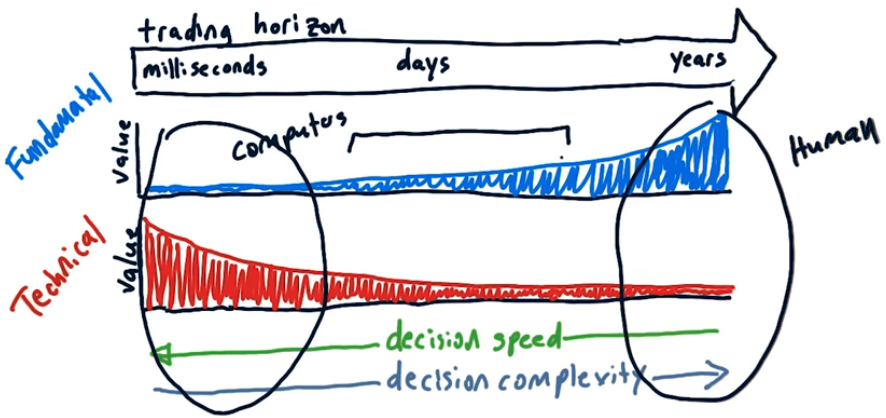
\includegraphics[scale=0.34]{fig/fig45}
\caption{When does technical analysis have value?}
\end{figure}

\textcolor{blue}{Decision complexity}: how complex is the decision to buy or sell a stock if you're going to hold it for years. It becomes more complex as time becomes longer. 

\textcolor{blue}{Decision speed}: how fast do the decisions have to be made? Certainly, we have to be able to make the decisions really really fast if we're trading at the millisecond level. And of course we can take a long time to make a decision if we're going to buy and hold for years. \\[8pt]
\noindent
As you look across this spectrum, consider where is the best region for humans to operate and where is the best region for computers to operate? Because at this very high frequency, the complexity of the decision is simple. Computers can make this decisions very, very fast and that also happens to be where technical analysis has value, which is the domain of the computer. 

Over the long time periods, where we can take a long time to make a decision and the decisions are complex. This is best region for human investors. 

So different types of hedge funds operate over different regions across the spectrum: the high frequency trading computer driven hedge funds are operating over the short time periods; the insight driven, human based hedge funds are operating on the other end of the spectrum. Over the region in the middle, humans and computers work together. 

\subsubsection{A few indicators}

Technical indicators are heuristic that represent someone's interpretation or hunch of how a statistical approach to previous prices and volume might suggest future price movement. There are hundreds of technical indicators out there. We look at three most common and most popular ones that people use: \\
(1) momentum \\
(2) simple moving average (SMA) \\
(3) Bollinger Bands\textsuperscript\textregistered \\[8pt]
\noindent
\textbf{Momentum} 

Momentum is one of the simplest indicators, and it's just over some number of days how much has the price changed. A positive momentum is when stock price has increased over the days, while negative momentum is when the stock price has decreased over the days. Connecting the two prices at the beginning and end dates of the days gives us a straight line, and the steepness of that line is the strength of the momentum, either positive or negative. 

To use this in a trading strategy, some people look at the recent momentum, if it's positive they buy, because they anticipate that the momentum is going to continue. We can use momentum as part of a combined strategy. 

\begin{figure}[!ht]
\centering
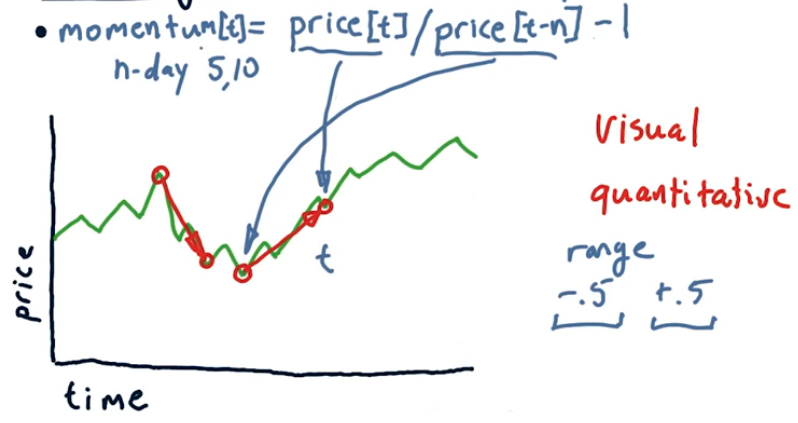
\includegraphics[scale=0.4]{fig/fig46}
\caption{Momentum}
\end{figure}

We have to convert the graphical/visual representation to quantitative representation in machine learning, for instance. 
\begin{equation}
\text{momentum[t]} = \frac{\text{price[t]}}{\text{price[t-n]}} - 1
\end{equation}
n-day is 5 or 10.  We usually see numbers in the range of about -0.5 for a significant drop to about 0.5. \\[18pt]
\noindent
\textbf{Simple moving average} 

SMA for today is simply the average of the values over the look back period (n-day). SMA looks essentially like a smoothed value of the price chart as it moves around. An important thing to note is it sort of lags the actual price movement.

\begin{figure}[!ht]
\centering
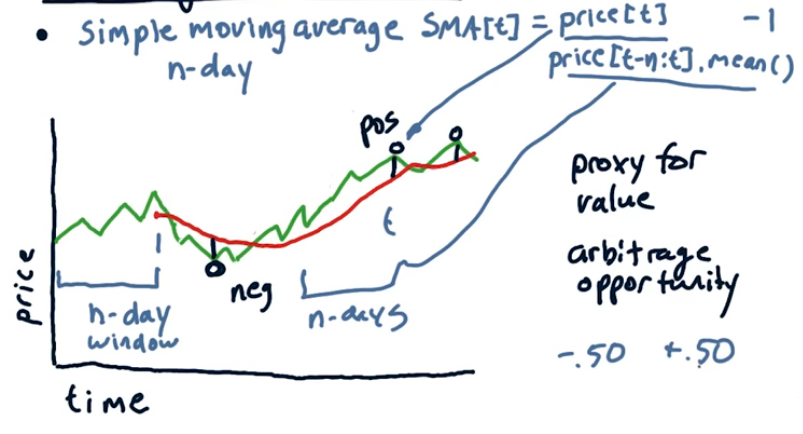
\includegraphics[scale=0.4]{fig/fig47}
\caption{Simple moving average}
\end{figure}

There are at least two ways that technicians use SMA as parts of trading strategies. The first is they look for places where \textcolor{blue}{the current price crosses through the simple moving average}. Those tend to be important events, especially if the average is over many, many days. If you combine them with momentum, in other words, the price has strong momentum, and it's crossing through that simple moving average, that can be a signal. 

Another way that technicians use \textcolor{blue}{simple moving average is as a proxy for underlying value}. In other words, if you look back over a certain period of time and take that average price, that might represent the true value of the company. And if we see a large excursion of the current price from that price, we should expect that the current price is eventually going to come back down to that average. So it's an arbitrage opportunity, sort like we saw with fundamental analysis. 

Quantitative representation of SMA 
\begin{equation}
\text{SMA[t]} = \frac{\text{price[t]}}{\text{price[t-n:t].mean()}} - 1
\end{equation}
It basically calculates what the change percentage of the current price from the simple average of the last $n$ days' price. Typical range of this value is between -0.5 and 0.5. \\[8pt]
\noindent
\textbf{Bollinger Bands\textsuperscript\textregistered} 

How much of an excursion from the simple moving average should I use as a signal for a buy or sell? John Bollinger observed that for low volatility stocks or stocks that are currently experiencing low volatility, you probably want to use a smaller number for that trigger, and when we see high volatility, you probably want to use a large number. To accomplish that, we can use the standard deviation. Bollinger suggested was that let's take this simple moving average, and let's add a band above and below two standard deviations. That's our measure how strong of a deviation we want to see before we respond to it. 

\begin{figure}[!ht]
\centering
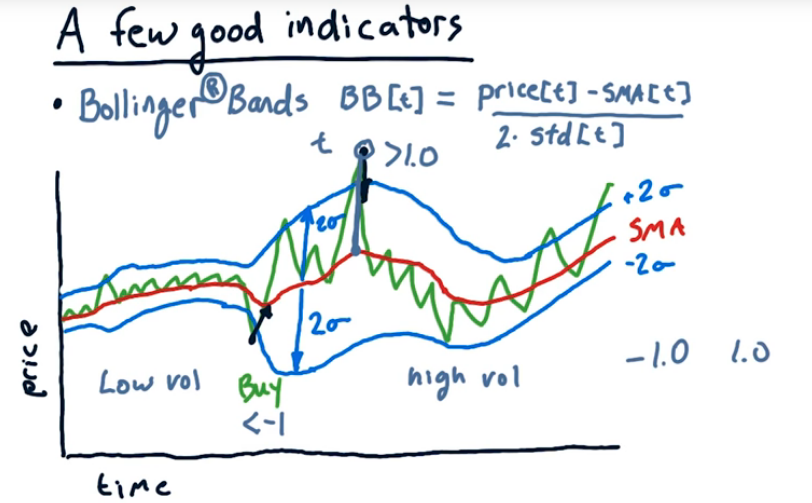
\includegraphics[scale=0.45]{fig/fig48}
\caption{BBollinger Bands\textsuperscript\textregistered}
\end{figure}

\noindent
How to use Bollinger Bands\textsuperscript\textregistered? \textcolor{magenta}{Look for cross from \textbf{outside} to \textbf{inside}}: \\
(1) You look for times where the price's outside one of these Bollinger Bands\textsuperscript\textregistered and when it crosses to the inside. These would be a sell signal. We've got a large excursion from the SMA, and we're expecting that it will retreat back to the average. \\
(2) Conversely, at places where the price's moving from below the lower band back towards the SMA, these would be a buy signal. 

To calculate Bollinger Bands\textsuperscript\textregistered on a particular day: 
\begin{equation}
\text{BB[t]} = \frac{\text{price[t]-SMA[t]}}{2\cdot\text{std[t]}}
\end{equation}
Typical values are in the range from -1.0 to 1.0, which mean most of the time the stock is going to be between these bands, but occasionally, we'll see excursions above and below those values. 

\subsubsection{Normalization}

Different indicators have different ranges. If we were to plug these values into some sort of machine learner, we would have a little bit of a problem. What would happen is the Bollinger Bands\textsuperscript\textregistered  factor would tend to overwhelm these other factors and become the most important one. It might even get worse if we included fundamental factor like PE ratio, which can range from 1 all the way up to 300. The solution is called normalization. 

\begin{figure}[!ht]
\centering
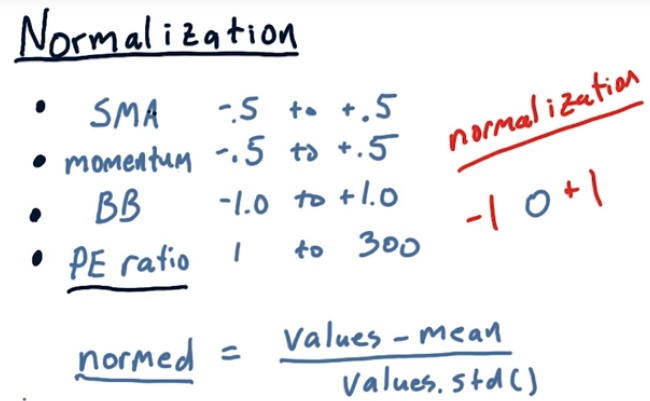
\includegraphics[scale=0.35]{fig/fig49}
\caption{Normalization}
\end{figure}

Normalization takes each of these factors and essentially compresses them or stretches them so that they vary on average from -1 to +1. 
\begin{equation}
\text{normed} = \frac{\text{values - mean}}{values.std()}
\end{equation}

%===================================================================================
\subsection{Dealing with data}

We work with historical price and volume data. 

\subsubsection{How data is aggregated}

\begin{figure}[!ht]
\centering
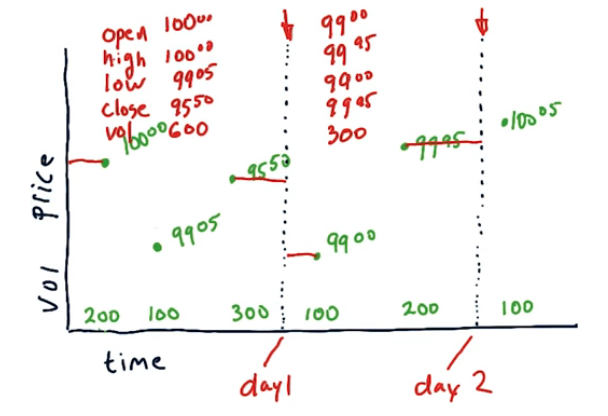
\includegraphics[scale=0.5]{fig/fig50}
\caption{How data is aggregated}
\end{figure}

Many trades are happening on different exchanges. How is all that data combined and how is it reported back to us so that we can analyze it and use it. The finest resolution of data is called a \textcolor{red}{tick}. A tick represents a successful buy-sell match or a successful transaction. Each exchange provides its own data feed regarding the transactions. So that you can subscribe to these feeds and see each tick when a transaction happens on any particular exchange. The prices and/or volumes on different exchanges might be different. All these are happening simultaneously, all the prices of different exchanges aren't guaranteed to be exactly the same. For highly liquid stocks, there may be hundreds or thousands of transactions every second. So collecting and using all these ticks for all the exchanges over a long period of time would result in a lot of data, and it becomes very complex. 

Tick data is usually consolidated into minute by minute or hour by hour chunks. Suppose the dash lines are minute boundaries, we collect all the data together within each minute, and represent it as open, high, low, close and volume. \textcolor{blue}{Open} is the first transaction within the time period. \textcolor{blue}{High} is the highest price within the entire time period. \textcolor{blue}{Low} is the lowest price within the time period. \textcolor{blue}{Close} is the last transaction. \textcolor{blue}{Volume} is just the total volume during that time period. 

Depending on your data feed, this aggregated data might be for one exchange or it might be combined across multiple exchanges. In this course, these time boundaries are in days. 

\subsubsection{Stock splits}

\textbf{Why?} \\ 
The only reason is that the price is too high. Why a price too high is a problem? People like to buy stocks in groups of 100. Another aspect is that options when they're traded on stocks are usually traded with regard to 100 shares. Options covering 100 shares of, say, \$500 stocks, become suddenly very expensive and less liquid. So from the point view of options and also individual stock shares, very high prices are a problem. Finally, one other issue is if you're building a portfolio and you want to have a finely tuned proportion of each stock in your portfolio. If some of the stock prices are very high, it becomes difficult to get that fine resolution that you want. \\[8pt]
\noindent
\textbf{Problems?} \\
If you want to trade using this actual closed data, you have to account for all these splits. Otherwise, the splits may be interpreted as short opportunities by your algorithms, while in fact the value of the company isn't decreasing, you just have more shares. \\[8pt]
\noindent
\textbf{Solution: Adjusted close} \\
At the very last day, in other words today, adjusted close and actual close are always the same. We track back in time and adjusted close and actual close are exactly the same. But on this day when we see 2 for 1 split, we go back over all the historical data, and we divide it all by 2, and then by 4 (thus 8 from that date backward) at the 1 for 4 splits. That continues back in time. As we go back we adjust for each of the splits in  history. 

\begin{figure}[!ht]
\centering
\includegraphics[scale=0.4]{fig/fig51}
\caption{Stock splits}
\end{figure}

\subsubsection{Dividends}

Many companies pay regularly dividends to their owners. A stock that's priced at say around \$100, can very often pay up to \$1 or \$2 per year in dividends, or 1 or 2\%. Some stocks pay even more than that. Dividends can have a significant effect on what happens to the actual price of the stock. 

\begin{figure}[!ht]
\centering
\includegraphics[scale=0.45]{fig/fig52}
\caption{Dividends}
\end{figure}

Let's suppose that the consensus on the value of the company is worth \$100 per share. Suppose on a future date we're going to get \$1 dividend, and one share of the stock is still supposedly worth \$100. What price will the stock converge to on the day before the dividend is paid and the day the dividend is paid? 

If you know that owning a particular stock on a certain day is going to give you \$1 in dividends, would you like to own it? How does that affect the demand (and subsequently, price) of the stock? How about the day the dividend is paid out --- would the demand for the stock remain the same after the payout?

What's going to happen is that the stock price is going to rise to \$101 because everybody know that on the next day, you're going to have one share of a stock worth \$100 and \$1. So, the total value of that is \$101. On the very next day, the price is going to drop by \$1. And everybody who held a share that day will have 1 share of stock and \$1, so their value continues at this \$101 level. \\[8pt]
\noindent
\textbf{Adjusting for dividends} 

Adjusted price as of today or the latest date in our data is always the same as the actual price. As we go back in time, it remains about the same until we hit one of these events like a dividends or a split. We treat, historically, the price in the same way as we do with this split. In other words, just before the dividend is paid, we adjust all of these prices down by the proportion of the dividend. So in the above case, we adjust everything down by about \%1 all the way back in history. 

\begin{figure}[!ht]
\centering
\includegraphics[scale=0.45]{fig/fig53}
\caption{Adjusting for dividends}
\end{figure}

A couple of other things to reiterate about adjustments. As of today, the adjusted close and close are exactly the same, but as you go back in time they begin to diverge. Another thing is that at a certain date back in history, adjusted closes might be different for the data gathered in 2015 and 2018. The adjusted close price today (2018) in Yahoo's data, will be different, most likely lower than the adjusted close for date, if you had gathered it in 2015. 

\subsubsection{Survivor bias}

In this class, we simulate the strategies we might develop. When you simulate your trading, you roll back in time, you look at that universe of stocks (e.g. S\&P 500), we apply your algorithm to choose which stocks you might buy. 

A very common mistake people make is that they look at the membership of that universe, as of today. Then they go back in time and they use that list of stocks for their strategy. So let's go back in time, we take the current list of the S\&P 500, and we run our strategy and our strategy is just doing great. The strategy is a \q{biased strategy}. Why is it biased? We're selecting from stocks way back in history that we knew were existing today, so there's a build in bias that these stocks are going to do well because they weathered the storm. 

Now consider, what if we use the S\&P 500 as it was back in 2007? A lot of the stocks from back then did just fine, they survived, but a lot didn't. 68 stocks from the S\&P 500 died. They completely went away from 2007 to 2009. So if you apply the same strategy that appears to be so awesome, but you use the real members of the S\&P 500 from back then, you're probably going to have a significantly lower performance. The difference between the two performances is the bias.

\begin{figure}[!ht]
\centering
\includegraphics[scale=0.45]{fig/fig54}
\caption{Survivor bias}
\end{figure}

The lesson learned is to use survivor bias free data and that's available from a number of providers. it's not usually free, but it's not necessarily that expensive either. But if you do that, you'll avoid this sort of false optimism for a strategy that you develop. 

%===================================================================================
\subsection{Efficient markets hypothesis}

For technical analysis we assume that there is information in historical price and volume data that we can discover and exploit in advance of the market. For fundamental analysis we assume there is information in fundamental data, like earnings that can be exploited and traded upon in advance of the market. The efficient markets hypothesis says we're wrong about both. 

\subsubsection{EMH assumptions}

The first ideas that eventually became the Efficient Markets Hypothesis (EMH) were postulated by Jules Regnault in 1863. Eugene Fama carried those ideas further in the 1960's, and it became his PhD thesis. Fama recently received a Nobel Prize. 

\begin{figure}[!ht]
\centering
\includegraphics[scale=0.45]{fig/fig55}
\caption{EMH assumptions}
\end{figure}

\noindent
\textbf{EMH assumptions} \\
\underline{(1) There are a large number of investors interacting in the market for profit.} So they have incentive to find opportunities, where the price of a stock is out of line with what its true value is. Because there are so many of these investors operating simultaneously, any time a little bit of information comes out there, the price is going to move. \\
\underline{(2) New information arrives randomly.} So it arrives at random times, it arrives at random rates for different stocks, but it's constantly arriving and investors are paying attention to that information and therefore the prices are adjusting quickly. \\
\underline{(3) Prices adjust quickly.} \\
\underline{(4) The current price reflects all available information.} In other words, all this information that's trickling in is acted upon by the investors, the price adjusts quickly to that information, and the current price reflects all of the information about that stock. 

\subsubsection{Origin of information}

Where does information come from? There's a number of places information can come from. Let's step through a few of these sorted from most public to least public. 

\noindent
(1) \textcolor{blue}{Price/volume}: This is public. It's rapid, it's quick, everybody can see it. This is the basis of technical analysis.

\noindent
(2) \textcolor{blue}{Fundamental data}: This is reported quarterly and everybody can see it as well. It's public, but it points more to the root of the value of the company than just the price/volume. 

\noindent
(3) \textcolor{blue}{Exogenous data}: That's a fancy name for a simple concept. It's just information about the world that affects the company. As an example, if we were looking at an airline stock, an exogenous piece of data that would affects the price of the airline stock is the price of oil. If the price of oil goes down, usually the price of the airline stock goes up because energy is the number one cost for airlines. 

\noindent
(4) \textcolor{blue}{Company insiders}: A very important and secretive type of information relates to company insiders. Let's suppose you're a CEO, and you know that this drug that you've invented is about to be improved. You might go buy shares of your stock because you think the price of your stock is going to go up because that drug is going to be approved. Depending on the circumstances, it may or may not be legal, but this reflects information that you have that people outside the company do not have. So this insider information is probably the least accessible of all these types, of course, and of most other types of information as well. 

\begin{figure}[!ht]
\centering
\includegraphics[scale=0.4]{fig/fig56}
\caption{Where does information come from?}
\end{figure}

Each of these information has a relationship to the efficient markets hypothesis. In particular there's three forms of efficient markets hypothesis. And these types of information relate to each of these three forms. 

\begin{figure}[!ht]
\centering
\includegraphics[scale=0.4]{fig/fig57}
\caption{Information relationship to the 3 forms of the EMH}
\end{figure}

\subsubsection{3 forms of the EMH}

There is three versions of the EMH that go from weak to strong. 

\begin{figure}[!ht]
\centering
\includegraphics[scale=0.4]{fig/fig58}
\caption{3 forms of the EMH}
\end{figure}

\noindent
\textcolor{red}{Weak:} Future prices cannot be predicated by analyzing historical prices. 

The idea here is that the current price reflects all information we might know. So just by looking at these historical prices you can't predict what is going to happen next. Notice, however, that this does leave room potentially for fundamental analysis. 

\noindent
\textcolor{red}{Semi-strong:} Prices adjust rapidly to new public information. 

So, for instance, when companies have their quarterly reports, that contain fundamental information, prices react immediately to that information. So, if semi-strong is correct, that would seem to prohibit even fundamental analysis. There's one possibility left though. One way that we might make money and that is based on insider information.

\noindent
\textcolor{red}{Strong:} Prices reflect all information public and private. 

We can't even make money on insider information. So if there's some secret information within the company that points to a higher price later, the price will go up in the face of that knowledge. So if the strong version of the EMH is true, it is essentially impossible to make money by holding a portfolio, other than the market portfolio. 

\subsubsection{Is the EMH correct?}

If it is, we can't beat the market using any of these strategies we might be looking at. There is evidence that certain versions of the hypothesis are not correct. And there are a number of very successful hedge funds out there that would seem to indicate that you can make money in the market by investing in things other than just the market portfolio. 

The strong version of the EMH is the least solid. In other words, the strong version of the EMH says that you can't even profit from insider information. The reason that it's not true is because we have seen people make money from insider information. Some of them have gone to jail, but clearly, it's a method that can provide profit, even though it might be illegal. 

\begin{figure}[!ht]
\centering
\includegraphics[scale=0.5]{fig/fig59}
\caption{Date set refutes the semi-strong version of the EMH}
\end{figure}

The following data set that seems to refute the semi-strong version of the EMH as well. Each dot represents the P/E (price/earning) ratio on a particular date on the horizontal axis; the vertical location is how much money did it make in terms of price over 20 years. A low P/E ratio is better, since it means a lower price but higher earnings. So, presumably, lower P/E values along the horizontal axis indicate higher value for a stock. 

Each group of colors represent different decade when the analysis was done. For instance, the dark blue was an analysis based on what the P/E ratios of stocks were in 1890 to 1910 and all the way up to the red, which was 1970 through 1985. For all of these decades, we saw at the beginning of the corresponding time period, low P/E ratios corresponded with higher returns. So this shows that price/earnings ratios are very predictive across many, many decades of future returns, and that tends to refute the semi-strong version of the EMH. 

%===================================================================================
\subsection{The fundamental law of active portfolio management}

Warren Buffet made a number of insightful comments over the years. One of my favorite is \q{only when the tide goes out do you discover who's been swimming naked.} The one for this lesson is \q{While diversification is only necessary when the investors do not know what they are doing.} Mr. Buffet is talking about two things: investor skill and breadth or the number of investments. This lesson is about how investment performance relates to those two factors.

\subsubsection{Grinold's fundamental law}

In the 1980s, Richard Grinold was seeking a method of relating performance, skill, and breadth in investing. For instance, you might be a skilled investor, meaning that you can pick up stocks well, but you might not have many opportunities or breadth to exercise that skill. Grinold developed a relationship he called \q{the Fundamental Law of Active Portfolio Management}. 
\begin{equation}
\text{performance} = \text{skill}\cdot\sqrt{\text{breadth}} 
\end{equation}
\begin{equation}
\text{IR} = \text{IC}\cdot\sqrt{\text{BR}}
\end{equation}
So if you want to improve your performance you can improve skill, or you can find more and more applications or methods or opportunities for applying that skill. As an example breadth might relate to how many stocks you invest in and skill relates to your skill in choosing them. 

Performance is summarized in something called information ratio, which is very much like the Sharpe ratio, but it refers to the Sharpe ratio of excess returns, in other words the manner in which the portfolio manager is exceeding the market's performance. Skill is summarized in something called information coefficient. Breadth is just how many trading opportunities we have. 

\subsubsection{The coin flipping casino}

We're going to explore these ideas in a thought experiment called \q{the coin flipping casino}. Two betting cases: case 1, we bet all 1000 coins on 1 table; in case 2, we bet the 1 coin on each of the 1000 tables.

\begin{figure}[!ht]
\centering
\includegraphics[scale=0.4]{fig/fig60}
\caption{The coin flipping casino}
\end{figure}

\noindent
\textbf{Reward and risk} \\
Both cases have the same reward/expected return \$20. \\
What is the chance you lose all the money? Case 1: 0.49; case 2: $0.49^1000$. \\
What is the standard deviation of individual bets? Case 1: 1.0; case 2: 31.62 (not exactly?) \\
What is reward/risk (Sharpe ratio)? Case 1: 20/31.62 = 0.63; case 2: 20/1 = 20. 

\begin{figure}[!ht]
\centering
\includegraphics[scale=0.4]{fig/fig61}
\caption{The coin flipping casino: risk}
\end{figure}

\begin{figure}[!ht]
\centering
\includegraphics[scale=0.4]{fig/fig62}
\caption{The coin flipping casino: reward and risk}
\end{figure}

\noindent 
\textbf{Observations and lessons} 

\begin{centering}
$20 = 0.63\cdot\sqrt{1000}$ \\
$\text{SR\_{case2}} = \text{SR\_{case1}}\cdot\sqrt{\text{bets}}$ \\
\end{centering}

If you split your bets evenly across multiple tables, this relationship will hold. in other words, the Sharpe ratio for Case 1 (betting 1000 coins on 1 table) is our base case, as we spread it out over more and more tables, the Sharpe ratio improves by the square root of that number of bets. This relationship exactly looks like the Fundamental Law of Active Portfolio Management. Namely, our overall performance is related to the skill in the case of making a single pick times the square root of the number of picks that we're able to make. 

You can improve things either by having more skill. In case of coin flips, skill is how biased is the coin; in the case of investing, it's how good are you at predicting the future return of the stock. Or you can improve your performance by increasing your breadth.

\begin{figure}[!ht]
\centering
\includegraphics[scale=0.4]{fig/fig63}
\caption{The coin flipping casino: observations and lessons}
\end{figure}

We come up with three lessons: One, higher $\alpha$ generates a higher Sharpe ratio; two, more execution opportunities provides a higher Sharpe ratio; three, Sharpe ratio grows as the square root of breadth. 

\subsubsection{The fundamental law}

Let's consider two real worlds funds: One is RenTec or Renaissance Technologies, which is funded by Jim Simons, a math and computer science professor, and he's had tremendous performance over the last several decades; and Warren Buffet, who runs Berkshire Hathaway. Both of the funds over the years have produced similar returns. But on the one hand, Warren Buffet holds maybe 120 stocks, and he doesn't trade much, he just holds them. Renaissance technology trades maybe 100,000 times per day. Can a single theory relate these two? \\[6pt]

\begin{figure}[!ht]
\centering
\includegraphics[scale=0.4]{fig/fig64}
\caption{The fundamental law: Buffet vs }
\end{figure}

\noindent
\textbf{IR, IC, Breadth} \\ [8pt]
\textcolor{red}{IR (Information Ration):}

\begin{centering}
$r_p(t) = \beta_pr_m(t) + \alpha_p(t)$ \\
\end{centering}

The return on our portfolio for a particular day is equal to the market component of the return, which is $\beta$ for that portfolio times the return on the market for that day, plus this residual return. Another way to look at that is to say that the market component of the return is due to the market, and the residual return is due to the skill of the fund manager. Remember, $\alpha$ is about skill.

\begin{figure}[!ht]
\centering
\includegraphics[scale=0.4]{fig/fig65}
\caption{Information ratio}
\end{figure}

We can calculate the Sharpe ratio of the skill component, just like we calculate the Sharpe ratio of an entire portfolio. Essentially, the Sharpe ratio of the skill component is the IR. 
\begin{equation}
\text{IR} = \frac{ \text{ mean(}\alpha_{\text{p} }(t)) }{ \text{ std(}\alpha_{\text{p} }(t)) }
\end{equation}
where $\text{mean(}\alpha_{\text{p}}(t))$ is our reward component, and $\text{std(}\alpha_{\text{p}}(t))$ is our risk component. It's calculated by looking back historically at the daily values of $\alpha$. We take the mean and the standard deviation of them over time. You can find these $\alpha$ by finding $\beta$ for the portfolio, calculating what the market return component was for each day, and then the difference is this residual or skill. 

This information ratio applies in many different cases, not just in this fundamental law case. People use information ratio as a measure of manager performance all the time. It's fair to say that IR is essentially a Sharpe ratio of excess return, the part that's due to skill. \\[5pt]
\noindent
\textcolor{red}{IC (Information Coefficient):} \\
IC, or the information coefficient is just the correlation of the manager's forecast to actual returns. So for instance, if she made a forecast on IBM, that would to u 1\%, and it went up 0.5\%, well, that's a positive correlation. This value can range from 0, where the correlation is not present, to 1, where it's very, very strong. \\[5pt]
\noindent
\textcolor{red}{BR (Breadth):}\\
Finally, BR, or breadth, represents the number of trading opportunities per year. So for example, if you're Warren Buffet, and you hold 120 stocks, and you just hold them all year, that's 120 trading opportunities. If, say, you are Jim Simons, and you trade 100,000 times per day, you multiply that times the number of trading days in a year, well, it turns out to be a very large number. Key thing is, even if it's just a portfolio where you buy and hold, you count the number of positions in that portfolio as the number of trading opportunities, because this is oriented around an annual measure. 

\begin{figure}[!ht]
\centering
\includegraphics[scale=0.4]{fig/fig66}
\caption{Information coefficient and breadth}
\end{figure}

\noindent
\textbf{The fundamental law} 

\begin{equation}
\text{IR} = \text{IC} \cdot \sqrt{\text{BR}}
\end{equation}

Grinold was able to show mathematically that information ratio is equal to information coefficient times the square root of breadth. So performance of the manager, or the fund, is due to the skill at making predictions times the square root of breadth. That means for instance, that you may be very skilled but you've got to have opportunities to invest in order to operationalize your skill. If you want to improve your performance you can either focus on improving your skill or focus on improving your breadth. Sometimes, it turns out, that it's a lot easier to increase breadth by finding additional stocks you might look at or additional markets. You might have some commodity trading strategy that works great. You can increase your breadth by looking at additional commodities. However, the strength of the this increase, in other words, as you increase breadth, the overall performance only increase at the square root of that breadth. So it tapers off after some amount of time. It turns out, though, that it's very, very hard to improve your skill, so that's why, for instance, folks often focus on the breadth component of this equation. 

%===================================================================================
\subsection{Portfolio optimization and the efficient frontier}

Suppose you have a set of stocks that you've determined are good investments. How much of your portfolio should you invest in each? There are many potential answers to that question. In this section we take a look at the approach called mean variance optimization, or portfolio optimization. The specific question we're looking to answer is this. \textcolor{blue}{Given a set of equities and a target return, find and allocation to each equity that minimizes risk.}

\subsubsection{What is risk?}

We use volatility as a measure of risk and that is simply the standard deviation of historical daily returns. That's the standard view of risk in most finance texts. There are other ways to view risk, but the key is standard deviation of daily returns. \\[8pt]
\noindent
\textbf{Visualizing return vs risk}  \\
We can build a portfolio by combing multiple assets, like the various stocks plotted in the figure and weighting each asset by a particular weight that represents its allocation within the portfolio. So each stock has a weight and when combined altogether, we end up with a portfolio that has properties of each of the stocks. It's typical got a risk somewhere in the middle and a return somewhere in the middle. 

\begin{figure}[!ht]
\centering
\includegraphics[scale=0.5]{fig/fig67}
\caption{Visualizing return vs risk}
\end{figure}

\subsubsection{Can we do better?}

For a long time, people build portfolios this way. They would look at a bunch of assets, essentially equally weight them, and end up with a portfolio that behaved somewhat in between. If you want a low-risk portfolio, you should focus on assets that are low-risk; if you wanted high return, you should focus on assets with high returns. Can we do better? Can we have a portfolio that has a return similar to the portfolio with a high return and has a risk similar to the one with a low risk at the same time? Indeed we can, and due to a man named Harry Markowitz, who won his Nobel Prize for his insight. 

What Markowitz discovered, and what people had been overlooking, was the relationship between stocks in terms of covariance. So the resulting performance of a portfolio, especially in terms of risk, is not just a factor, or a blend of the various risks, but it has to do with how they interact day to day. So indeed, \textcolor{blue}{if we pick the right stocks in the right proportions, we can get a portfolio that in fact can have lower risk than any of the individual assets.}

Up until the time of his discovery, most people viewed bonds as the lowest risk asset, in other words, if you wanted low risk, you should use bonds only. Markowitz showed that a blend of stocks and bonds is actually lower risk than either one of those by themselves. 

\subsubsection{Why covariance matters?}

To illustrate the importance of covariance, we take a look at a couple different stocks. Both ABC and GHI have gone up 10\%. GHI tends to zig when ABC zags, so it's not going in lockstep with ABC. DEF goes almost in lockstep with ABC. So , three stocks, two that move together very similarly, and one that moves opposite them sometimes, yet they've all provided about 10\% return. What is the best portfolio we can build by combining these three different stocks?

Let's consider their covariance, or how they move together, for a moment. So ABC and DEF move very similarly. If we measure their correlation coefficient, $\rho = \frac{Cov(ABC, DEF)}{\sqrt{Var(ABC)Var(DEF)}}$, say, 0.9. While for ABC and GHI it is -0.9. 

Let's consider a couple different portfolios, which are just weightings on these different assets. Let's first look at one that is 50\% ABC and 50\% DEF. They both move similarly, so this portfolio is going to track the two of them together. There is no real advantage of blending these two assets because it just has the same volatility as each one them by themselves. 

What if we take 25\% of ABC, 25\% of DEF, but we put the rest of it in GHI? So we're combining an anticorrelated asset with these other two. The portfolio is going to be a nice blend of them, with very low volatility, because when one zigs, the other zags. So this portfolio will also have a 10\% return, but it is much smoother---lower volatility than any asset by itself. So all these assets by themselves had significant volatility, but when we put them together, we reduced volatility significantly. 

\begin{figure}[!ht]
\centering
\includegraphics[scale=0.4]{fig/fig68}
\caption{Covariance matters}
\end{figure}

\subsubsection{Mean variance optimization (MVO)}

What Markowitz added to the game was this consideration of variance and co-variance between individual stocks, and the recognition that you want to blend those together that have anti-correlation, so you can have a much lower risk portfolio if you combine assets that are anti-correlated. Because when one moves up, the other moves down, they cancel each other out, and you have much less volatility. Of course, you want all these assets to, in general, move up together. So often \textcolor{blue}{what we are looking for is anti-correlation in the short term and positive correlation in a longer term.}

Out of this work grew a number of algorithms. One of the key ones being mean variance optimization, which is a way of taking a potential set of assets and figuring out how they should be blended together by looking at their co-variance among other things. One thing needs to be pointed out is that generally the higher return stocks or assets tend to also be the highest risk. So as well roll down the risk we tend to also look at lower return. How can we combine these into a good portfolio?

\begin{figure}[!ht]
\centering
\includegraphics[scale=0.45]{fig/fig69}
\caption{Mean variance optimization}
\end{figure}

Here is what goes into a mean variance optimizer:\\
(1) Expected return: For each stock, you have to provide an expected return. In other words, what do we think in the future it's going to provide in terms of return. \\
(2) Volatility: Volatility simply historically how volatile has each one of the assets been. \\
(3) Covariance: Covariance is a matrix which shows between each asset and every other asset, what is the correlation of daily returns. \\
(4) Target return: The last and perhaps one of the most important inputs is the target return. We can target a return anywhere from the max return asset and min return asset. And then anything else between those, of course, we can accomplish by blending. 

The output of an optimizer is a set of weights, one weight for each asset, that provides the target return but minimizes the risk. Let's suppose the dotted line in the figure is our target return; in the end we're looking for a portfolio represented by the orange dot.  In other words, it's got risk that's even lower than any of the individual assets, but it meets the target return. This is possible because we consider covariance. If we're only looking at individual risk, we wouldn't be able to find the right blend. 

\subsubsection{The efficient frontier}

Here we look at one last topic with regard to portfolio optimizers and modern portfolio theory. Consider these assets, and also recognize that for any particular return level, there is an optimal portfolio. 

Let's suppose we pick this return level, and this is the optimal portfolio (see orange dot in the figure). In other words, this portfolio reflects weightings of all these assets that provides the lowest risk for this particular return. Now, we can compute this for all the potential returns, from the minimum return stock up to the maximum. If we did that for all of them, you get a line. 

\begin{figure}[!ht]
\centering
\includegraphics[scale=0.45]{fig/fig70}
\caption{The efficient frontier}
\end{figure}

A couple of different things to observe that are interesting. One is as you reduce the return sometimes this curve comes back, indicating that actually the risk is increasing as we reduce return. So for the most part, people don't want those sorts of portfolios. In other words, who wants a lower returning portfolio with more risk. We typically look only at portfolios above the orange line. The name of the curved line is \q{the efficient frontier}. There is no portfolios possible outside the curve, and any portfolio below the curve is sub-optimal in some way, because it's either higher risk or lower return than it could be if we were on the efficient frontier. 

One last thing to mention about the efficient frontier is if you draw a tangent line from the origin to the frontier where it hits is the max Sharpe ratio portfolio for all these assets. In practice the efficient frontier isn't used for that much other than as a theoretical device, but people do often like to plot the efficient frontiers so they can see where their portfolio is in relation to the assets that they're using and where they could be in terms of efficiency. 


%%%%%%%%%%%%%%%%%%%%%%%%%%%%%%%%%%%%%%%%%%%%%%%%%%%%%%%
\newpage
\section{Learning Algorithms for Trading}

%===================================================================================
\subsection{How Machine Learning is used at a hedge fund?}

This section introduces how hedge funds and other financial institutions utilize machine learning. In general, the focus is on creating a model that can be used to predict future prices for stocks or other assets. Models like these have been around for a long time. What's different about machine learning is that it provides a suite of tools that support a data-centric way to build predictive models. 

\subsubsection{The ML problem}

Scientists like to talk about the algorithms they build in terms of the problem the solve, so this mini course is about machine learning and let's think about the problem the machine learning solves. In most cases, machine learning algorithms are focused on building a model. 

What's a model? A model is something that takes in observations like $x$, run it through some sort of process, and provide a $y$. This $y$ is typically a predication, and the $x$ is some sort of observation of the world. Examples might be, for us, $x$ are some features of stocks and $y$ is a future price. There are many other uses of machine learning models. That's just one of them. $x$ can be multidimensional. In other words, there might be multiple factors that we're considering, might be Bollinger Bands\textsuperscript\textregistered, PE ratio, and so on. $y$ is typically single dimension and just represents that single-dimension prediction that we're trying to make. 

\begin{figure}[!ht]
\centering
\includegraphics[scale=0.45]{fig/fig71}
\caption{The ML model}
\end{figure}

There are lots of models that people have built that don't use machine learning at all. One example is the Black-Scholes model that predict option prices. There are many other types of models that predict things that people build not using machine learning, but they develop mathematical formulas. But, of course, with machine learning, we're trying to use data. So the machine learning process is to take historical data, run it through a machine learning algorithm of some sort to generate the model. Then at runtime or when we need to use the model, we push $x$'s in it and $y$'s come out. 

\subsubsection{Supervised regression learning}

The particular flavor of machine learning that we're going to focus on in the first part of this course is called supervised regression learning. All that \textcolor{red}{regression} means is we're trying to make a numerical approximation or a numerical predication. That's opposed to classification learning where we might be trying to classify an object into one of several types as opposed to making a numerical predication. \textcolor{red}{Supervised} means that we show the machine the $x$ and also, if you will, the correct answer $y$. In fact, we show the machine many, many examples of $x$ and $y$, and that's how it learns when I see this $x$, this is the $y$ that's associated with it. \textcolor{red}{Learning} means that we are training with data. In this class we're taking historical stock data and training the system to make a predication about the future, usually about price. 

\begin{figure}[!ht]
\centering
\includegraphics[scale=0.45]{fig/fig72}
\caption{Supervised regression learning}
\end{figure}

There are lots of algorithms that solve this problem and are supervised regression learning techniques. \\
(1) You've probably heard of linear regression and used it. \textcolor{blue}{Linear regression} is a method that finds parameters for a model. So we call it parametric learning. \\[8pt]
(2) \textcolor{blue}{K nearest neighbor (KNN)} is an extremely popular approach. What's different between \underline{Parametric learning and instance based} (e.g., KNN) is that parametric learning we take the data, munge it around to come up with a few parameters, and then throw the data away; in K nearest neighbor we keep all of this historical data, the $x$ and $y$ pairs, and when it's time to make a predication we consult that data, that's what makes it instance based. \\[8pt]
(3) Two other techniques that are really popular are decision trees and decision forests. As you might guess, the way \textcolor{blue}{decision trees} work is they store a tree structure and when a query comes in, it essentially bounces down that tree according to factors of the data. Each node in the tree represents essentially a question, is this $x$ value greater than or less than this other value? And eventually we reach a leaf and that is the regression value that's returned. \textcolor{blue}{Decision forests} are simply lots and lots of decision trees taken together, and you query each one to get an overall result. 

\subsubsection{How it works with stock data}

This is one of our Pandas data frames that contains some factors or features of stocks, and it's arranged in the usual way where each column represents the value of the feature for a particular stock. And time goes downward essentially. We might have many features for each stock, for instance we might have Bollinger Bands\textsuperscript\textregistered, momentum, PE ratio, and so on. We represent that by stacking these one behind the other. These are potentially multidimensional. These are our $x$'s.

What is our $y$? In most cases, we want to use our historical feature data to predict a future price. But to train our model, we're going to use historical price as well. So the values of these factors or features we call $x$ and we like to be able to run that through the model that we've built and get $y$, which is our predicted future price. 

\begin{figure}[!ht]
\centering
\includegraphics[scale=0.45]{fig/fig73}
\caption{How it works with stock data}
\end{figure}

We don't have that model yet, we're going to learn it. And we're going to learn it from data. Here is how we do that. We roll back time so that we'er back in history at our first data point. We look at the values of our features there, and then we look, say, 5 days into the future to see what the future price is. So now we've got a pairing of these features with the future $y$. We save that $<x, y>$ pair into our data. And that's one instance of data. We move forward one day. So we've got a new set of $x$'s and a new $y$. And we record that in our database. Eventually, we reach a point where we can't go any further because there's no more $y$ data. In any case, we now, for each of these days in history, have a pair of $x$'s and $y$'s that we can feed into our database to build our model. 

\subsubsection{Example at a FinTech company}

This sections shows how we use this process to build a machine-learning based forecaster at a FinTech company, Lucena Research. The first step is to select which factors do you want to use? So those are our $x$'s. So these are things like Bollinger Bands\textsuperscript\textregistered, PE ratio, and so on (measurable quantities about a company that can be predictive of its stock price). The next step is to select what is it you want to predict? Usually we want to predict change in price, market relative change in price, or for now we could just think that as future price. These both become our data, our $x$'s and our $y$'s that we used to train the model. 

Now that we know what our predictive factors are and what $y$ is going to be, we need to consider the breadth and depth of data that we're going to use to train the system with. So that includes, for instance, time period. How far back in time do you want to go to train the system? And what's your stock universe? What universe of data, which symbols are you going to use to train the system as well?

\begin{figure}[!ht]
\centering
\includegraphics[scale=0.45]{fig/fig74}
\caption{Example at a FinTech company}
\end{figure}

Now we can train our model. We can take this data to produce that model. We unleash our machine learning algorithm. This might be KNN, linear regression, or decision tree. That algorithm takes this data and converts it into a model. 

We're ready now to use that model to do some prediction. The way we do that is we measure the quantities about the stocks that we want to make a prediction for now. We measure what those $x$'s are today, plug those into the model and the model should provide us our $y$, or our prediction. 

\subsubsection{Price forecasting demo}

This is a cloud-based application called QuantDesk. I was developed by a company called Lucena Research. Over on the left there are various lists of stocks that you can choose from. When you choose, for example, Dow Jones, you can see a list of stocks that make up that group of stocks. 

Over the lower left corner are our forecasting options, and this is how we tell the machine learning algorithm which factors we want to use, how far in the future we want to predict, and so on. The default model has the list of factors that the developers think are important for making a future price prediction. It turns out that these factors are determined using another machine learning algorithm. They use a genetic algorithm for discovering these. 

As an example, we make a one month forecast and use three months of data. So we're going to be looking back three months at all these factors. When we roll back time, we're able to see the future price of these stocks, so we can see how those factors presumably affected the future price. In the lower middle we have a forecast for Apple. We can see the historical price, looking back the last three months, and the forecast future price. So that line is indicating that we think it's going to go up, and this arc line above and below is our confidence interval. 

\begin{figure}[!ht]
\centering
\includegraphics[scale=0.35]{fig/fig75}
\caption{Price forecasting demo I}
\end{figure}

We also report that data in a tabular format up in the top. It shows the current price, forecast change in price, and forecast percentage change, etc. So the system thinks that from today Apple is going to go up about 2.5\%. 

We also report some other information over the top right corner. We report what we call confidence and back tests score. \textcolor{red}{Confidence} refers to when we find those $K$ nearest neighbors, how diverse are the $y$'s that comes back? So, $K$ is the number of neighbors, and when we look at all those neighbors, that are the closest to the values of quantities that Apple has today, we find the 30 closest ones, and we look at the standard deviation among all those 30. If they're very close, we're confident in our prediction; if they're spread apart, we're less confident. 

So you can see here, American Express is a more confident prediction, and we rate this by a number of stars, by the way, where five stars represent our most confident estimates and one star, of course, our least confident. So our system thinks American Express is going to go down by 0.9\% over the next month. It's got a high confidence, and it's also got a high back test score. So what's this \textcolor{red}{back test score}? What we do is we roll back time, and we look over all this last three months and look forward one month. And we see how accurate all those predictions were over the last three months. The more accurate those were, the higher ranking we get there.  

\begin{figure}[!ht]
\centering
\includegraphics[scale=0.35]{fig/fig76}
\caption{Price forecasting demo II}
\end{figure}

\subsubsection{Backtesting}

The natural question is how accurate are these forecasts? Can you act on them? Do they really predict the future? At least a first step towards answering that question can be found by backtesting. So that means that you roll back time, and you test your system. 

\begin{figure}[!ht]
\centering
\includegraphics[scale=0.45]{fig/fig77}
\caption{Backtesting}
\end{figure}

So here's our historical data, it's organized with time coming down. In order to test the capability of our approach, we have to limit the data it sees to a certain amount of time and then make predictions into the simulated future. So we allow our system to only look at data up to a certain point. It can use data before that all it likes. It builds a model, and then makes a forecast. On the basis of that forecast, we can then now place orders, anticipating that that forecast will be achieved. So we might long some stocks or short them as appropriate. We can take those orders now, put them into our trading simulator and see how the portfolio works. We enter our positions on that date and we roll it forward and see what happens with the portfolio. Using software that we've built in this class, you can measure things like Sharpe ratio, return, and so on for that portfolio. 

Now we're training over new data, make a new forecast and then make a new set of orders. We enter these orders in our trading simulator and then go forward and see what happens. This process can be repeated over and over again using historical data and we can simulate our learning algorithm and how it would trade in this way. That's called backtesting. \\[8pt]
\noindent
\textbf{Backtesting in a real system}

On the QuantDesk platform, we can backtest in the exactly the same way. Go over here to the Backtest tab and click on Forecast. And again we can configure which group of stocks are we going to work with, and what are the setting for our backtest. For instance, how much money do we start with? How frequently do we want to trade, over what period of time do we want to run the backtest and so on. Anyways, we make those selections. 

We also need to choose parameters for the forecaster. Again, which model do we want to use, which includes what are the factors that we're paying attention to, how far into the future do we want to make our forecast and how much data looking back do we want to use. Once we make all those selections, we can click on Backtest and it'll start running. 

\begin{figure}[!ht]
\centering
\includegraphics[scale=0.35]{fig/fig78}
\caption{Backtesting in a ML system}
\end{figure}

Here's an example report that the system generates. This is for a forecast backtest. The orange line here represents the historical value of our portfolio; the blue is the benchmark that we're using, which is S\&P 500. Over the right are a number of metrics tabulated. Over this period of time we saw 346\% return. Our Sharpe ratio was 1.14 and so on. 

\begin{figure}[!ht]
\centering
\includegraphics[scale=0.5]{fig/fig79}
\caption{Report of backtesting in a ML system}
\end{figure}

\subsubsection{Problems with regression}

As you saw by that backtest, regression-based forecasting can be useful. It's also worth noting that that particular backtest was not spectacular. It did indeed beat the S\&P 500, which is important, but it didn't beat it spectacularly. Usually we find that performance in the real world is not as awesome as in backtesting. So we would probably still see good return from that strategy but it wouldn't be quite the same as we saw in that backtest. 

Here is a list of problems we see sometimes with regression-based forecasting. \\
(1) First of all, our forecasts always seem to be noisy and uncertain. So there is value in there, but it has to be accumulated over many trading opportunities. \\
(2) It's hard to know how confident you should be in a forecast. We mentioned in the software demo that we could look at standard deviation of the nearest neighbors. That works okay. It's really not too strong of a measure, however. So it's difficult to know how confident you ought to be in any particular forecast. It would be nice if you could know because that would enable you to essentially bet less on forecasts that are less certain. \\
(3) Additionally, it's not clear how long you should hold a position that might have risen from a forecast, and how you should allocate to that position. 

Some of these issues can be addressed using reinforcement learning, where instead of making a forecast of a future price, we had the system learn a policy and the policy tells the system whether to buy or sell a stock. It's an interesting alternative to the regression based approaches. 

\begin{figure}[!ht]
\centering
\includegraphics[scale=0.45]{fig/fig80}
\caption{Problems with regression}
\end{figure}

\subsubsection{Problem we we will focus on}

We're going to look at a certain period of data, train our models over that period, and then make forecasts and trade over some other period. Here's our historical data. We're going to use the period of 2009 as our data to train our model. You'll be implementing several machine learning algorithms to create different models and will be comparing them one against another. Then we'll test over the years 2010 and 2011. So those testing values will become our $x$, which will push through the model to create a $y$ or a forecast. And using this forecast you'll generate an orders.txt file, which you can push through your market simulator. We'll see how that strategy performs, measuring its Sharpe ratio and its total return and so on. And that way we'll be able to compare different machine learning algorithms that generate these orders. 

\begin{figure}[!ht]
\centering
\includegraphics[scale=0.45]{fig/fig81}
\caption{Problem we we will focus on}
\end{figure}

%===================================================================================
\subsection{Regression}

Regression here means using data to build a model that predicts a numerical output based on a set of numerical inputs. 

\subsubsection{Parametric regression}

Parametric regression is a way of building a model where we represent the model with a number of parameters.

Suppose we want to build a model that will predict how much it will rain today based on changes in barometric pressure. We can use linear regression to fit a line to barometric pressure $x$ and rain $y$ and get a linear model $y = mx+b$. Instead of a line, we can fit a polynomial $y=m_2x^2 + m_1x + b$. Once we get the parameters, we throw away the data, and the model is represented just by these 3 parameters. We can add more terms to the model. In general, these parametric approaches come away with a number of parameters, and the more complex the model, the more parameters. 

\begin{figure}[!ht]
\centering
\includegraphics[scale=0.45]{fig/fig82}
\caption{Parametric regression}
\end{figure}

\subsubsection{K nearest neighbor}

There is another approach, it's a data-centric approach or instance based approach, where we keep the data and we use it when we make a query. 

As an example, let's suppose our barometric pressure has gone down by 5 millimeters and we want to consult our model to see how much it's going to rain today. Let's suppose $k=3$. So we will find the 3 nearest historical data points to this query. Since we are trying to predict $y$ (rain) at given $x$ (change in pressure), using the mean of nearest observed $y$ values makes sense. 

\begin{figure}[!ht]
\centering
\includegraphics[scale=0.4]{fig/fig83}
\caption{K nearest neighbor}
\end{figure}

If we were to repeat this process at many, many points along the $x$-axis, we end up with a model. The line interpolates nicely and smoothly between all the data points. There are number of methods like this that keep the data around and when they make a query, they consult the data to find the answer. The most famous of these methods is \textcolor{red}{K nearest neighbor}. But here are others, such as \textcolor{red}{kernel regression}. The main way that KNN differs from kernel regression is that in kernel regression we weight the contributions of each of the nearest data points according to how distant they are. Where as with KNN each data point that we consider gets essentially an equal weight. 

\subsubsection{Parametric vs non-parametric}

For a parametric approach, we don't have to store the original data, so it's very space efficient, but we can't easily update the model as more data is gathered. Usually we have to do a complete rerun of the learning algorithm to update the model. Thus for parametric approaches, training is slow but querying is fast. Parametric approaches have to assume a certain type of model, such as linear or quadratic and so on (\textcolor{red}{biased}).  

For non-parametric approaches, or instance-based, we have to store all the data points. So it's hard to apply when we have a huge data set, but new evidence can be added easily, since no parameters need to be learned. Adding data points doesn't consume additional time. Thus training is fast, but querying is potentially slow. Most importantly, these non-parametric approaches avoid having to assume a certain type of model (\textcolor{red}{unbiased}), whether it's linear or quadratic or so on. Therefore, they're suitable to fit complex patterns where we don't really know what the underlying model is like. 

\begin{figure}[!ht]
\centering
\includegraphics[scale=0.45]{fig/fig84}
\caption{Linear regression vs KNN}
\end{figure}

\subsubsection{Training and testing}

Consider the data that we're going to use. We're going to have features that we've computed, these are things like Bollinger Bands\textsuperscript\textregistered, momentum, price change and things like that. We're going to use these features to try and predict prices or price changes. So our $x$ data has got multiple features, thus is multidimensional $x_1$, $x_2$, $x_3$, and so on. $y$ data is what we try to predict. 

In order to evaluate our learning algorithms in a scientific manner, we need to split this data into at least two sections: a training section and a testing section. If we trained over the same data that we tested over, the results would be suspicious because we should obviously be able to do very well if we test over the same data we trained on. This procedure of separating testing and training data from one another is called \q{out of sample testing}. This is a very important and essential technique. 

We'll call the $x$ data that we use for training, $xtrain$ and the $y$ data that we use for training, $ytrain$. Similarly, the data we'll test on will be split into $x$ and $y$ sections, $xtest$ and $ytest$. The general idea here is that we'll take our $xtrain$ data and our $ytrain$ data, run that through our machine learning algorithm, which might be linear regression or KNN to generate a model. We can then test the accuracy of that model using the test data. So the input to the model is $xtest$, so plug that $x$ data into the model, and outcomes some kind of $y$. So the question is, is that $y$ equal to this $ytest$, which we know is ground truth. So the more closely the model outputs a $y$ that reflects this $xtest$ data, the more accurate the model is. 

\begin{figure}[!ht]
\centering
\includegraphics[scale=0.4]{fig/fig85}
\caption{Training and testing}
\end{figure}

It's worth to mention that we typically split the data according to time. So we train our model on older data and test it on newer data. There are certain look-ahead biases that can occur if you were to train on later data and test on earlier data.  

\subsubsection{Learning APIs (application programming interface)}

To write machine learning algorithms, it's useful if we standardize on what the application programming interface ought to look like for the code you're going to write. 
\begin{lstlisting}[language=Python, caption=]
"""For linear regression:"""
# A constructor that creates an instance of one of these learners, learner.
learner = LinRegLearner() 
# A method called train that can take our training data and train the model.
learner.train(Xtrain, Ytrain)
# A query function that takes a list of X values that you want to test and returns a list of Y values according to what the model thinks they should be. These Y values, in turn, are the ones that we'll compare to Ytest to see how well the algorithm works. 
Y = learner.query(Xtest)
"""For KNN:"""
# Our KNN ought to have the same methods. The only difference is the constructor here has this additional argument, K, which allows you to set how large you want K to be. 
learner = KNNLearner(k=3)
learner.train(Xtrain, Ytrain)
Y = learner.query(Xtest)
\end{lstlisting}

\begin{lstlisting}[language=Python, caption=]
"""Pseudo code for implementing API for a linear regression learner. The KNN API is going to look exactly the same."""
class LinRegLearner:
    def __init__():
        # For the linear regression learner, we don't have to do anything when we instantiated an instance of the learner
        pass 
        
    def train(X, Y):
        # Our training method takes an X and a Y, where X can be multidimensional. It takes in X and Y, and tries to fit a line to it. So it's trying to find an m and a b. 
        self.m, self.b = favorite_linreg(X, Y) 
        # self.m means the m goes to the local instance, and b to the local instance, and you're allowed to use any number of linear regression algorithms at your disposal as part of SciPy and NumPy. 
        
    def query(X):
        # X is passed and it's supposed to compute predicted Y given that X. 
        Y = self.m * X + self.b
        return Y
\end{lstlisting}

%===================================================================================
\subsection{Assessing a learning algorithm}

In KNN, if $k=1$, we have the most overfit model. As we increase $k$, we're less and less likely to overfit as we go forward. 

\begin{figure}[!ht]
\centering
\includegraphics[scale=0.45]{fig/fig86}
\caption{A closer look at KNN and parametric regression}
\end{figure}

For parametric models, increasing $d$ increases model complexity, and results in our model trying to closely align with the given data points. As we go off the edge of the parametric models, we're able to extrapolate in the direction the data seem to be going. This is the capability that parametric models or these polynomial models have that KNN does not. 

\subsubsection{Metric 1: RMS error}

We use error to measure the ways the models can fit the data more or less closely. A standard way to measure error is called RMS error. It is an approximation of the average error, but we end up emphasizing larger errors a bit more. 

\begin{figure}[!ht]
\centering
\includegraphics[scale=0.35]{fig/fig87}
\caption{RMS error}
\end{figure}

\noindent
\textbf{In sample vs out of sample}\\
In-sample error is the prediction error on training data that the model has already seen. Whereas out-of-sample error is based on unseen test data.

From KNN we know that we can build models that can fit the training data exactly. So we can have arbitrarily small error against our training set. The more important measure is, what is our error out of sample? Out-of-sample means we train on our training set, but we test on a separate testing set of data. That's going to be different from our training set. To measure out-of-sample error, we look at the error from our testing set, not our training set. \\ [8pt]
\noindent
\textbf{Cross validation and roll forward cross validation} \\
Usually when researchers are evaluating a learning algorithm, they split their data into two chucks: a training chunk and a testing chunk. Training usually is about 60\% of the data, and testing is about 40\%. If you train and then test on that data, that's one trial, and in many cases that's enough, you measured your RMSE and that's an assessment of your algorithm. You might compare it against another algorithm. 

One problem researchers sometimes encounter is they don't have enough data to effectively analyze their algorithm. One thing they can do is effectively create more data by slicing it up and running more trials. What we can do is we can slice our data into, say, five different chunks, and then we can train here on 80\% of the data, and test on 20\%. That's one trial. Then we can switch things up and train on this 80\% of the data, and test on that. That's another trial, and so on. We can effectively get five different trials out of this one set of data. 

\begin{figure}[!ht]
\centering
\includegraphics[scale=0.4]{fig/fig88}
\caption{Roll forward cross validation}
\end{figure}

Cross validation is a great tool, but the typical usage of it doesn't fit financial data applications well. The reason is that it can permit peeking into the future. For instance, if our training data is after our test data. That means we're seeing the future ahead of our test. Any sort of peeking like this can read to unrealistically optimistic results, so with sort of data we need to avoid it. One way to avoid this problem is with role forward cross validation. That means our training data is always before our testing data, but we can still have multiple trials just by rolling our data forward until we run out of data. 

\subsubsection{Metric 2: correlation}

Another way to visualize and evaluate the accuracy of a regression algorithm is to look at the relationship between predicted and actual value of our dependent variable $y$. Query our model, the one that we trained on our training data, with $xtest$, our testing data set. The output of that query is a new vector of $y$ values, $ypredict$. So based on this $xtest$ data our model predicts this $ypredict$ data. 

We can now compare what we know to be correct or true data, $ytest$, with what our prediction was. We can plot the $ypredict$ and $ytest$ pairs as a scatter plot. If the scatter plot is arranged in approximately a nice line, that means we've got a pretty good prediction algorithm. On the other hand, if they've not aligned so well, our leaner is not so good. We can measure this property quantitatively using correlation. You can use the NumPy function np.corrcoef() to measure the correlation between $ytest$ and $ypredict$. The value is in the range of [-1, +1], where +1 means they're strongly correlated. -1 means they are inversely correlated, and 0 means there's essentially no correlation at all between them. 

\begin{figure}[!ht]
\centering
\includegraphics[scale=0.4]{fig/fig89}
\caption{Correlation}
\end{figure}

One thing to point out here is that correlation isn't the slope. Correlation has to do with how well aligned the points are with the line that we fit. So if it's a nice oval that fits close to that line, we usually have a high correlation; if it's a big round thing we've got poor correlation. 

In most cases, as RMS error increases, correlation goes down. But yes, there are some cases where the opposite might happen (e.g. when there is a large bias).

\subsubsection{Overfitting}

Let's consider parameterized polynomial models, where we can, one at a time, add additional factors, like $x$, $x^2$, $x^3$, $x^4$, and so on. We create a graph, where along the horizontal axis we have degrees of freedom, or $d$, the degree of our polynomial. And vertically, we'll have the error of our model. Let's measure error as we increase $d$ on our training set. At one point, as we increase degrees of freedom, our in-sample error is decreasing, but our out-of-sample error is increasing. That's how we define overfitting. That's the region where overfitting is occurring. 

\begin{figure}[!ht]
\centering
\includegraphics[scale=0.4]{fig/fig90}
\caption{Parametric regression overfitting}
\end{figure}

KNN overfitting is different. When k = 1, the model fits the training data perfectly, therefore in-sample error is low (ideally, zero).  Out-of-sample error can be quite high. As k increases, the model becomes more generalized, thus out-of-sample error decreases at the cost of slightly increasing in-sample error. After a certain point, the model becomes too general and starts performing worse on both training and test data.

\begin{figure}[!ht]
\centering
\includegraphics[scale=0.4]{fig/fig91}
\caption{KNN overfitting}
\end{figure}

%===================================================================================
\subsection{Ensemble learners, bagging and boosting}

In 1988, Micheal Kearns and Leslie Valiant posed the following question. Can a set of weak learner be combined to create a single, strong learner? One answer to that question came in 2009. Back in 2006, Netflix offered a \$1 million prize for machine learning algorithm that could do 10\% better than their own algorithm at predicting which movies their customers would like to see. The prize was not awarded until three years later in 2009. The winning algorithm was not a single algorithm, but a combination of several, or an ensemble. This lesson is about ensemble learners. 

\subsubsection{Ensemble learners}

Creating an ensemble of learners is one way to make the learners you've got better. We're not talking about creating a new algorithm, but instead of assembling together several different algorithms or several different models to create an ensemble learner. We have multiple learners. We might have a KNN based model, a linear regression based model, a decision tree based model, and a support vector machine (SVM) based model. They're all trained with the same data, and so now we have, in this case, four different models. 

To query this ensemble of learners, we query each model by itself and combine the answers. So if we wanted to query this model with $x$, we plug $x$ into each model, the same $x$ and then our $y$s come out. So we have a $y$ output from each of these models, how do we combine them? If we're doing classification where for instance we're trying to identify what the thing is, we might have each of these $y$s vote on what it is. But we're doing the regression, and so the typical thing to do here is to take the mean, and that is the result for this ensemble learner. 

We can then test this overall ensemble learner using this test data that we set aside. 

\begin{figure}[!ht]
\centering
\includegraphics[scale=0.45]{fig/fig92}
\caption{Ensemble learners}
\end{figure}

Why ensembles? Why do we use them, why might they be better? There are a few reasons. First of all, ensembles often have lower error than any individual method by themselves. Ensemble learners offer less overfitting. The ensemble learners typically do not overfit as much as any individual learner by itself. Why is that? An intuitive answer is that as each kind of learner that you might use has a sort of bias. For instance, with linear regression our bias is that the data is linear. But when you put them together you tend to reduce the biases because they're fighting against each other in some sort of way. 

\subsubsection{How to build an ensemble of learners?}

\noindent
\textbf{Method I: Combine several models of different types} 

If we combine several models of different types (here parameterized polynomials and non-parameterized kNN models), we can avoid being biased by one approach. This typically results in less overfitting, and thus better predictions in the long run, especially on unseen data.

\begin{figure}[!ht]
\centering
\includegraphics[scale=0.45]{fig/fig93}
\caption{Create an ensemble of learners I}
\end{figure}

\noindent
\textbf{Method II: Bootstrap aggregating--bagging}

There's another way we can build an ensemble of learners. We can build them using the same learning algorithm but train each learner on a different set of the data. This's called \q{bootstrap aggregating} or \q{bagging}. It was invented by Bremen in the late '80s, early '90s. 

Here is how bagging works. What we do is we create a number of subsets of the data. The little bags in the figure represent bags of data. Each one of these is a subset of the original data. How do we collect these? We do it randomly. For each subset $D_m$ it contains $n'$ values, and our original data set contains $n$ different instances. We grab $n'$ of them, at random, with replacement from the original data. What replacement means is we might grab the same data as we grab $n'$ data from the $n$ values for each bag. We create all together $m$ of these groups or bags. Each one of them contains $n'$ different data instances chosen at random with replacement. In most implementations, $n' = n$. Because the training data is sampled with replacement, usually about 60\% of the instances in each bag are unique.

\begin{figure}[!ht]
\centering
\includegraphics[scale=0.5]{fig/fig94}
\caption{Create an ensemble of learners II}
\end{figure}

We use each of these collections of data to train a different model. We have now $m$ different models, each one trained on a little bit of different data. Just like when we have an ensemble of different learning algorithms, here we have an ensemble of different models we query in the same way. We query each model with the same $x$ and we collect all of their outputs. We take the $y$ output of each model, take their mean, and that's our $y$ for the ensemble. 

We can wrap this in a single API just like the API you wrapped your LinRegLearner() and your KNNLearner(). \\[8pt]
\noindent
\textbf{Bagging example}

A 1NN model (KNN with k = 1) matches the training data exactly, thus overfitting. An ensemble of such learners trained on slightly different datasets will at least be able to provide some generalization, and typically less out-of-sample error.

\begin{figure}[!ht]
\centering
\includegraphics[scale=0.45]{fig/fig95}
\caption{Bagging example}
\end{figure}

\subsubsection{Boosting: Ada Boost}

Boosting is a fairly simple variation on bagging that strives to improve the learner by focusing on areas, where the system is not performing well. One of the most well-known algorithms in this area is called Ada Boost, where Ada stands for adaptive. 

Here is how Ada Boost works. We build our first bag of data in the usual way. We select randomly from our training data. We then train a model in a usual way. The next thing we do is something different. We take all our training data and use it to test the model. We are going to discover that some of the points are not well predicted. So there are some points here, for which there is significant error. 

When we go to build our next bag of data, again, we choose randomly from our original data, but each instance is weighted according to this error. So the points that had significant error are more likely to get picked and go into this bag than any other individual instance. We ended up with a few of those point in the bag and a smattering of all the other ones as well. We build the model from this data and then we test it. Now, we test our system altogether. In other words, we've got a sort of miniature ensemble here, just two learners. We test both of them. We test them by inputing again this in-sample data and combine their outputs. And again we measure error across all this data. Maybe this time, some points got modeled better, but there were other ones that weren't as good. 

Thus we build our next bad and our next model. We just continue this over and over again up until $m$ or the total number of bags we'll be using. 

\begin{figure}[!ht]
\centering
\includegraphics[scale=0.45]{fig/fig96}
\caption{Ada Boost}
\end{figure}

To recap, bagging, when we build one of these instances, is simply choosing some subset of the data at random with replacement, and we create each bag in the same way. Boosting is an add-on to this idea, where in subsequent bags we choose those data instances that had been modeled poorly in the overall system before. 

As m increases, AdaBoost tries to assign more and more specific data points to subsequent learners, trying to model all the difficult examples. Thus, compared to simple bagging, it may result in more \textcolor{red}{overfitting}.

\subsubsection{Summary: Boosting and bagging}

Bagging and boosting are just methods for taking existing learners and essentially wrapping them in this meta algorithm that converts your existing learner into an ensemble. You should use the same API to call your ensemble that you would have earlier been using to call an individual learner. So externally, to whatever part of your program is calling the learner, it doesn't know underneath there you're doing boosting or bagging. Your resulting learner is also likely to have lower error and reduced overfitage. 

\begin{figure}[!ht]
\centering
\includegraphics[scale=0.4]{fig/fig97}
\caption{Boosting and bagging}
\end{figure}

To summarize, boosting and bagging are not new algorithms in and of themselves. They're meta algorithms that let you wrap your underlying algorithms into something that's better. 

%===================================================================================
\subsection{Reinforcement learning}

Up until this point, we've focused on learners that provide forecast price changes. We then buy or sell stocks with the most significant predicted price change. This approach ignores some important issues, such as the certainty of the price change. It also doesn't help us know when to exit the position either. In this lesson, we'll look at reinforcement learning. Reinforcement learners create policies to provide specific direction on which action to take. 

\subsubsection{The RL problem}

It's important to point out that when we say reinforcement learning, we're really describing a problem, not a solution. In the same way that linear regression is one solution to the supervised regression problem, there are many algorithms that solve the RL problem. First, let's explain this in terms of a problem for a robot. 

Our robot observes the environment by taking in some form of description of the environment, which is called the state $S$. The robot has to process that state somehow to determine what to do. We call this $\pi$ or policy, so the robot takes in the state $S$ and then outputs an action $a$. $a$ affects the environment in some way and changes it. The environment then transitions to a new state. $T$ is the transition function that takes in what the previous state was and the action and moves to a new state. And the new state comes out and back into the robot. Robot looks at his policy, action comes out. In robotics, we call this the sense-think-act cycle. You don't have to implement it only using reinforcement learning. 

How do we arrive at this policy? How do we find $\pi$? This whole puzzle (i.e. the cycle) is missing a piece and that's the thing that helps us find $\pi$. And part of that piece is called $r$, which is the reward. So every time the robot is in a particular state and it takes an action. There's a particular reward associated with taking that action in that state and that reward comes into the robot. The robot's objective is, overtime, to take actions that maximize this reward. Somewhere in the robot, there's an algorithm that takes all this information over time to figure out what that policy ought to be.  

\begin{figure}[!ht]
\centering
\includegraphics[scale=0.35]{fig/fig98}
\caption{The RL problem}
\end{figure}

To recap, $S$ is the state of our environment, that's what the robot senses in order to decide what to do. It uses its policy $\pi$ to figure out what that action should be. $\pi$ can be a simple lookup table. Over time, each time the robot takes an action, it gets a reward and it's trying to find the $\pi$ that will maximize its reward over time. 

In terms of trading, our environment really is the market and our actions are actions we can take in the market, like buying and selling or holding(?). $S$ are factors about our stocks that we might observe and know about. And $r$ is the return we get for making the proper trades.

\subsubsection{Mapping trading to RL problem}

First of all the environment is really the market. Our state includes things like market features, prices, whether we're holding the stock. Our actions are buy and sell, and potentially do nothing is also an allowable action. 

Let's think about this in the context of trying to learn how to trade a particular stock. We've got this historical time series, and say the vertical line is today. We can look back over time to infer the state of the stock, so what are the Bollinger Bands\textsuperscript\textregistered values and things like that. We process that and decide what's our action. Let's suppose that we decide to buy. Once we buy, we're now holding long. That's part of our state. We go forward, we're now on a new state, where the price has gone up. We're holding long, let's suppose we decide to sell at that point. So we've had two actions, well we've been in two states in state one we were not holding. We executed the action buy and went forward in time, and we're holding long now, and then we execute the action sell. Note that we've made money by taking the buy-then-sell action, and that's our reward $r$.

\begin{figure}[!ht]
\centering
\includegraphics[scale=0.35]{fig/fig99}
\caption{Mapping trading to RL problem}
\end{figure}

To recap, the policy that we learn tells us what to do at each time we evaluate state. We're going to learn the policy by looking at how we accrue money or don't based on the actions we take in the environment. 

\subsubsection{Markov decision problems}

Let formalize what we've been working with. It's called a Markov decision problem. Here're what make up a Markov problem. \\
(1) There are a set of states $S$. Those are all the values that this $S$ can take as it comes into the robot. \\
(2) There is a set of actions $A$. They are the potential actions we can take to act on the environment. \\
(3) There is the transition function $T[s, a, s']$. This is the $T$ within the environment. $T$ is a three-dimensional object, and it records in each of its cells the probability that if we are in state $a$ and we take action $a$, we will end up in state $s'$. Something to note about this transition function is, suppose we're in a particular state $s$ and we take a particular action $a$, the sum of all the next states we might end up in has to sum to one. In other words, with probability one, we're going to end up in some new state, but the distribution of probabilities across these different states is what makes this informative and revealing. \\
(4) Finally, an important component of Markov decision problems is the reward function $R[s, a]$. If we are in a particular state and we take action $a$, we get a particular reward. 

\begin{figure}[!ht]
\centering
\includegraphics[scale=0.42]{fig/fig100}
\caption{Markov decision problems}
\end{figure}

If we have all of these things defined, we have what's called a Markov decision problem. The problem for a reinforcement learning algorithm is to find this policy $\pi$ that will maximize reward over time. In fact, if it finds the optimal policy, we give it a little symbol $\pi^\ast$ to indicate that it's optimal. 

If we have these, and, in particular, if we have $T$ and $R$, there are algorithms we can unleash that will find this optimal policy. Two of them are \textcolor{red}{policy iteration} and \textcolor{red}{value iteration}. In this class, we don't start off with $T$ and $R$, we're not going to be able to use these algorithms directly to find this policy. 

\subsubsection{Unknown transitions and rewards}

Most of the time we don't have this transition function, and we don't have the reward function either. The robot, or the trader, whatever environment we're in, has to interact with the world, observe what happens, and work with that data to try to build a policy. For example, let's say we are in state $s_1$, that's what we observe there. Our robot took action $a_1$, we then find ourself in $s'_1$, and we get reward $r_1$. $<s_1, a_1, s'_1, r_1>$ is an experience tuple. This is very similar to experience tuples in regression learning, where we have an $x$ and a $y$ paired together; it's an experience tuple of when you observe this $x$ and you see this $y$. Here, we're saying when you observe the state $s_1$, you take action $a_1$, you end up in this new state, at least it's an example of you ending up in this new state $s'_1$, and reward $r_1$. 

Now we find ourselves in a new state $s_2$, but that's really $s'_1$, where we found ourselves. We take some new action $a_2$, we end up in some new state $s'_2$, and we get a new reward $r_2$. We do this over and over again, gathering experience tuples all along the way. 

\begin{figure}[!ht]
\centering
\includegraphics[scale=0.42]{fig/fig101}
\caption{Unknown transitions and rewards}
\end{figure}

If we have this trail of experience tuples, there's two things we can do with them in order to find that policy $\pi$. The first set of approaches is called model based reinforcement learning. What we do is we look at this data over time and we build a model of $T$ just by looking statistically at these transitions. In other words, we can look at every time we were in a particular state and took a particular action, see which new states we ended up in, and just build a tabular representation of that. Similarly, we can build a model of $R$. We just look statistically when we're in a particular state, and we take an action, what's the reward? We can just average that over all these instances. Once we have these models, we can then use value iteration or policy iteration to solve the problem. 

There's another set of approaches called model-free. That's the type we're going to focus on. In particular, we're going to learn about Q-learning. Model-free methods develop a policy just directly by looking at the data. 

\subsubsection{What to optimize?}

We didn't go into enough detail about what it is we're trying to optimize here. We just said something vague like we want to maximize the sum of our reward. It's not so simple, in fact, here's a great story to illustrate that. There's a great Russian comedian, Yakov Smirnoff. He told this joke once. He said have you heard about the Soviet lottery, it's a million rubles if you win, one ruble a year for a million years. So the point is that one dollar or one ruble delivered to us a million years in the future is really not as valuable as a dollar or ruble that we get now. So, for instance, if we think about a robot living forever, it might do something just mundane to gather a dollar a year. That's an infinite amount of money, but in practice it doesn't really work that well. So to consider that and illustrate that, let's see a little maze problem, and we'll think about what the robot ought to do that would be optimal in this maze. 

We have our robot and a challenge. We have a reward of \$1 and a reward of \$1 million in the maze. If the robot comes over the \$1 bin, it gets the reward, it's special in that each time it touches, it gets \$1 and it goes away but then it comes back. So the robot could come here, go back and forth, and get a dollar each time it moves here. As for the \$1 million bin, once the robot tags it, it's gone. But clearly it's worthwhile to come over here and grab it. The red area is obstacle, it can't go there. The numbers are the penalties the robot would get as it went over them.

Let's say that what we want to optimize is the sum of all future rewards, then it doesn't matter whether we go the way to just get that dollar over and over again, or if we go the other way to get the one million dollar, and come back and get that \$1 over and over again. There's no difference because they both sum to infinity over time. 

What if we want to optimize out reward over three moves. So we've got a finite horizon. Let's consider the rewards we get with a finite horizon of three if we go one way versus the other way. If we go toward the \$1 million, we're going to get rewards of -1, -1, -1; if we go the other way, we get 0, 1, and then move down and get another 0. Then the best thing to do is go towards the \$1. If we extend the horizon a little bit further, say out to eight, then going towards the \$1 million is the best thing to do. So clearly as we expand our finite horizon trivially up to say eight step, going towards the \$1 million is the best thing to do. If we carried it even further, we'd discover that then we should come back towards the \$1 and go to that dollar and tag it over and over again. 

\begin{figure}[!ht]
\centering
\includegraphics[scale=0.45]{fig/fig102}
\caption{What to optimize?}
\end{figure}

To formalize it, with the infinite horizon what we're trying to maximize is the sum of all rewards over all of the future. So it's the sum of each of these rewards for $i$ equal to 1 to infinity. The finite horizon is very similar, it's just we don't go to infinity. So for optimizing over horizon of four steps, $n$ would be 4. 

There's yet another formulation about what's the value of a future dollar. If it takes us, say, four years to get a dollar, that dollar is less valuable than say if it takes one year. The same way, if it takes, say, eight steps to make a dollar, that dollar is less valuable than a dollar I can get just in one step. 

The way we represent that is very simple, just like we represented the sum of future dividends and it's called discounted reward, $\sum_{i=1}^{\infty}\gamma^{i-1}\cdot r_i$. So instead of just summing up the $r_i$, we multiply it by this factor $\gamma^{i-1}$, such that our immediate reward, the very next one we get, whatever $\gamma$ is when it gets raised to the zeroth power is just one. So that means for the very next step we get $r$, but for the step after it, it's $\gamma$ to the one, so it devalues that reward a little bit. 

$\gamma$ is a value between 0 and 1. The closer it is to 1, the more we value rewards in the future. The closer it is to 0, the less we value rewards in the future. In fact, if $\gamma$ is set equal to 1, this is exactly the same as the infinite horizon. But $\gamma$ relates very strongly to interest rates if you recall. So, if say, $\gamma$ were 0.95 it means each step in the future is worth about 5\% less than the immediate reward if we got it right away. This is the method we use in Q-learning. One reason is that the math turns out to be very handy, and it provides nice conversion properties. 

\subsubsection{Summary}

\noindent
(1) The problem for reinforcement learning algorithms is a Markov decision problem (MDP). Reinforcement learning algorithms solve them. \\
(2) A Markov decision problem is defined by $S$, $A$, $T$, and $R$, where $S$ is the potential states, $A$ are the potential actions, $T$ is the transition probability, which is given I'm in state $s$, I take action $a$, what' the probability I'll end up in state $s'$, and $R$ is the reward function. \\
(3) The goal for reinforcement learning algorithm is to find a policy $\pi$ that maps a state to an action that we should take, and its goal is to find this $\pi$ such that it maximizes some future sum of the reward. We talked about that bing either infinite horizon, fixed horizon, or discounted sum. \\
(4) We can map our task for trading to reinforcement learning and it works out like this. $S$, our states, are features about stocks and whether or not we're holding a stock. Actions $A$ are buy, sell, or do nothing. The transition function $T$ is the market, and finally, the reward function $R$ is how much money we get at the end of a trade. So we can apply reinforcement learning algorithm to find this policy. We mentioned a few of the algorithms, for instance, policy iteration, and value iteration, and $Q$-learning, but we haven't talked in detail what they are, and that's the subject of lessons coming up. 
 
\begin{figure}[!ht]
\centering
\includegraphics[scale=0.4]{fig/fig103}
\caption{Summary}
\end{figure}

%===================================================================================
\subsection{$Q$-Learning}

$Q$-learning is a model-free approach, meaning that it does not know about or use models of the transitions $T$or the rewards $R$. Instead, $Q$-learning builds a table of utility values as the agent interacts with the world. These Q-values can be used at each step to select the best action based on what it has learned so far. The fantastic thing about $Q$-learning is that it is guaranteed to provide an optimal policy. There is a hitch, however, that we'll cover later. 

\subsubsection{What is $Q$?}

$Q$-learning is named after the $Q$-function. What is that? $Q$ can be written as a function. so we might have parentheses around $s$ and $a$, or you can think of it as a table. In this class, we're going to view $Q$ as a table. 

It's got two dimensions, $s$ and $a$. $s$ is the state we're looking at, and $a$ is the acton we might take. $Q$ represents the value of taking action $a$ in state $s$, and there's two components to that. The two components are the immediate reward that you get for taking action $a$ in state $s$, plus the discounted reward. The discounted reward is the reward you get for future actions. 

An important thing to know is that $Q$ is not greedy, in the sense that it just represents the reward you get for acting now. It also represents the reward you get for acting in the future. 

\begin{figure}[!ht]
\centering
\includegraphics[scale=0.4]{fig/fig104}
\caption{What is $Q$?}
\end{figure}

Let's suppose we have $Q$ already created for us. We have this table. How can we use it to figure out what to do? So what we do in any particular state is the policy. And we represent the policy with $\pi$. So $\pi(s)$ means, what is the action we take when we are in state $s$, or what is the policy for state $s$? We take advantage of our $Q$ table to figure that out. Here's how it works. We are in state $s$ and we want to find out which action is the best. All we need to do is look across all the potential actions and find out which value of $Q[s, a]$ is maximized. So we don't change $s$, we just step through each value of $a$, and the one that is the largest is the action we should take. The mathematical way to represent this is to use the function \q{argmax()}. What is does is it finds the $a$ that maximizes $Q$, and then the answer is $a$.

After we run $Q$-learning for long enough, we'll eventually converge to the optimal policy. We represent that with a little star. This is how to use a $Q$-table if you have it. We need now to consider how do we build that $Q$-table in the first place.  

\subsubsection{Learning procedure}

Here's the big picture at a high level of how we train a $Q$-learner. We have time series of stock market data, and it's arranged from oldest to newest vertically in the graph. We select which data we want to train on, then we iterate over this data over time. We evaluate the situation there, and for a particular stock that gives us our state $S$. We consult our policy $\pi(s)$ and that gives us an action $a$. We take that action and plug it into our system, evaluate the next state, and we get $s'$ and our reward $r$. 

After one iteration, we've got an $s$, an action $a$, an $s'$, and an $r$, or an experience tuple $<s, a, s', r>$. We use that experience tuple to update our $Q$-table. Once we get all the way through the training data, we test our policy and we see how well it performs in a backtest. If it's converged or it's not getting any better then we say we're done. If now, we repeat this whole process all the way through the training data. 

What do we mean by converge? Each time we cycle through the data, training our $Q$-table and then testing back across that same data, we get some performance. We expect that each time we complete an iteration, our performance is going to get better and better. But after a point it finally stops getting better and it converges. Eventually we reach this regime, where more iterations don't make it better and we call it converged at that point. 

\begin{figure}[!ht]
\centering
\includegraphics[scale=0.4]{fig/fig105}
\caption{$Q$-learning procedure?}
\end{figure}

Here are the details as we iterate over our training data. (1) We start by setting our start time, and we initialize our $Q$-table. The usual way to initialize a $Q$-table is with small random numbers, but variations of that are fine. (2) At the start time, we observe the features of our stock or stocks and from those we build up together our state $s$. (3) We consult our policy, or in other words we consult $Q$-table to find the best action in the current state. That gives us $a$. (4) Then we step forward and we see what reward we get and what's our new state. (5) We now have a complete experience tuple that we can use to update our $Q$-table. So we take this information we just learned and we improve $Q$ based on that information. Then we step to the next point in time and the next point time and so on. 

\subsubsection{Update rule}

Consider our robot here that's interacting with the world. The first thing it sees is some state, then takes that state, goes look in the $Q$-table, and finds the action that corresponds to the maximum $Q$. It takes that action. Once that action is taken, that results in two new things: one is a new state $s'$, and a reward $r$. All that information comes into the robot, and it needs to use that information to update its $Q$-table. As a consequence of this interaction with the world, it's got an $s$, and $a$, an $s'$, and an $r$.

How does it take that information to improve this $Q$-table? There are two main parts to the update rule. The first is, what is the old value that we used to have? That's $Q[s, a]$. And what is our improved estimate? We want to blend them together. To combine them, we introduce this new variable $\alpha$. $\alpha$ is the learning rate. $\alpha$ can take on any value from 0 to 1. Usually we use about 0.2. What that means is in our new improved version of $Q$, which is indicated as $Q'$, it's a blend of $\alpha$ times the improved estimate, plus $1-\alpha$ of the old value. So larger values of $\alpha$ cause us to learn more quickly, lower values of $\alpha$ cause the learning to be more slow. So a low value of $\alpha$, for instance, means that in this update rule, the previous value for $Q[s, a]$ is more strongly preserved. 

Stretching it out a little bit more detail, we have our current value for the $Q$ at $s$ and $a$ plus $\alpha$ times the immediate reward $r$, plus $\gamma$ times later rewards. $\gamma$ is the discount rate. Similar to $\alpha$, $\gamma$ usually ranges from 0 to 1. A low value of $\gamma$ means that we value later rewards less. Recall the discount rate when we were talking about bonds, it's the same thing. A low value of $\gamma$ equates to essentially a high discount rate. A high value of $\gamma$, in other words a $\gamma$ near 1, means that we value later rewards very significantly. If we were to use 1.0, that means a reward 20 steps in the future is worth just as much as a reward right now. 

We have to expand the later rewards component in a little bit more detail. This component represents our future discounted rewards. In other words, we end up in state $s'$, and from then on out, we're going to act optimally, or at least, the best that we know how to. The question is, what is the value of of those future rewards if we reach state $s'$ and we act appropriately? It is simply that $Q$ value, but we have to find out what the action is that we would taken, so that we can reference the $Q$-table properly. So if we're in state $s'$, the action that we would take that would maximize our future reward is argmax$_{a'}$, where $a'$ is the next action we're going to take. So we're going to find that best $a'$ that maximizes the value when we're in that state $s'$. The argmax$_{a'}(Q[s', a'])$ collapses to $a'$, then we look up the $Q$-table value for $Q[s', a']$.

So our update rule is the following. Our new $Q$ value in state $s$, action $a$ is that old value multiplied by $1-\alpha$ (depending on how large $\alpha$ is, we value that old value more or less), plus $\alpha$ times our new best estimate. Our new best estimate is our immediate reward plus the discounted reward for all of our future actions. 

\begin{figure}[!ht]
\centering
\includegraphics[scale=0.45]{fig/fig106}
\caption{Update rule}
\end{figure}

The formula for computing $Q$ for any state-action pair $<s, a>$, given an experience tuple $<s, a, s', r>$, is:
\begin{equation}
Q'[s, a] = (1 - \alpha) \cdot Q[s, a] + \alpha \cdot (r + \gamma \cdot Q[s', \text{argmax}_{a'}(Q[s', a'])])
\end{equation}
\begin{description}[font=$\bullet$\scshape\bfseries]
\item $r = R[s, a]$ is the immediate reward for taking action a in state s, \\[-35pt]
\item $\gamma \in [0, 1]$ is the discount factor used to progressively reduce the value of future rewards,\\[-35pt]
\item $s'$ is the resulting next state, \\[-35pt]
\item $\text{argmax}_{a'}(Q[s', a'])$ is the action that maximizes the $Q$-value among all possible actions $a'$ from $s'$, and \\[-35pt]
\item $\alpha \in [0, 1]$ is the learning rate used to vary the weight given to new experiences compared with past $Q$-values.
\end{description}

\subsubsection{Two finer points about $Q$-learning}

\begin{description}[font=$\bullet$\scshape\bfseries]
\item The success of $Q$-learning depends to a large extent on exploration. We need to explore as much of the state and action space as possible. One way to accomplish this is with randomness. The way we can interject that fairly easily in the step of $Q$-learning, where we are selecting an action, we flip a coin and randomly decide if we're going to randomly choose an action. That means two flips of the coin. The first is are we going to choose a random action or are we just going to pick the action with the highest $Q$-value? If we decide we're going to choose an action randomly, then we need to flip the coin again to choose which of those actions we're going to select. 
\item Typical way to implement this is to set this probability at about 0.3 or something at the beginning of learning. Then over each iteration to slowly make it smaller and smaller until eventually we essentially don't choose random actions at all. What we gain here is when we're choosing these random actions fairly frequently is we're forcing the system to explore and try different actions in different states. It also causes us to arrive at different states that we might not otherwise arrive at if we did't try those random actions. 
\end{description}

\begin{figure}[!ht]
\centering
\includegraphics[scale=0.45]{fig/fig107}
\caption{Two finer points}
\end{figure}

\subsubsection{The trading problem}

Let's consider how we can turn the stock trading problem into a problem that $Q$-learning can solve. To do that we need to define our actions, state, and rewards. \\[8pt]
\noindent
\textbf{Actions}

Let's first start here with actions. We just have three actions: buy, sell, or do nothing. Let's consider how that might play out with an actual stock, and let's suppose we've already trained our $Q$-learner what to do. Usually what's going to happen most frequently is that we do nothing. There will occasionally be buys and sells, but usually nothing. 

So we are evaluating the factors of the stock. In other words, we compute, say, several technical indicators. That is our state. We consider that state and we do nothing. Let's suppose we do nothing for quite a long period here, but somehow after a little while, something triggers and says we should buy. So we buy the stock here (green vertical line), we're holding it. We do nothing for a long while, and then our $Q$-learner says, it's time to sell (red vertical line). We continue like that through the rest of our time series. 

\begin{figure}[!ht]
\centering
\includegraphics[scale=0.45]{fig/fig108}
\caption{The trading problem: actions}
\end{figure}

Let's consider how these buys and sells affect our portfolio value. We start with whatever we've got in the bank and there's no trading for a while. Suddenly there's a buy, and then we see an increase in our portfolio value until we hit that sell. Then nothing. Again, another buy, and a sell. And nothing. So you see this sort of stepped behavior. In this illustration, we're choosing opportunistic times to buy and sell.  In reality, your real strategy is probably not going to be so good, but ideally this's the kind of thing we'd like to see.  \\[8pt]
\noindent
\textbf{Rewards}

Rewards should relate in some way to the returns of our strategy. There are at least two approaches that we can utilize. Short-term rewards in terms of daily returns or long-term rewards that reflect the cumulative return of a trade cycle from a buy to a sell, or for shorting from a sell to a buy. 

Consider these two, (1) daily returns or \textcolor{red}{immediate reward}, where each day we get a reward, which is equal to the return over the last day, or (2) \textcolor{red}{delayed reward}, where the reward is equal to zero, until we exit the position, then the cumulative return that we gained across that whole trade. Which one of these will result in faster convergence?

\begin{figure}[!ht]
\centering
\includegraphics[scale=0.4]{fig/fig109}
\caption{The trading problem: rewards}
\end{figure}

Daily return is the answer.  If we reward a little bit on each day, the learner is able to learn much more quickly because it gets much more frequent rewards. A reward at each step allows the learning agent get feedback on each individual action it takes (including doing nothing).

If we get no reward at all until the end of a trade cycle, from a buy to a sell, the learner has to infer from that final reward all the way back that each action in sequence must have been accomplished in the right order to get that reward. \\[8pt]
\noindent
\textbf{State}

What factors make sense to be in the state?

\begin{figure}[!ht]
\centering
\includegraphics[scale=0.45]{fig/fig110}
\caption{The trading problem: state}
\end{figure}

Adjusted close is not a good factor for learning, because you are not able to generalize over different price regimes for when the stock was low to when it was high. Also, if you're trying to learn a model for several stocks at once and they each hold very different prices, adjusted close doesn't serve well to help you generalize. Same thing is true for simple moving average (SMA). However, if you combine adjusted close and SMA together into a ratio that makes a good factor to use in state. 

Bollinger Band\textsuperscript\textregistered value and P/E ratio are also good. 

A new kind of feature that we're considering with reinforcement, is whether we're holding the stock or not. That's an important state to know, in other words, if you're holding the stock, it may be advantageous to get rid of it. But if you're not holding it, you might not necessarily want to sell. So this additional feature about what your position is is useful.

Similarly, return since we entered the position might be useful. In other words, this might help us set exit points for instance, maybe we've made 10\% on the stock since we bought it and we should take our winnings while we can. 

\subsubsection{Creating the state}

An important consideration in what we're doing here is that our state is a single number. It's an integer. That way we can address it in our cue table. It's certainly the case that some reinforcement learning methods are able to treat the state as a continuous value. To get started here, let's use state as an integer so we can work more easily with the data. 

Here is a general way to get our state to an integer. Our first step is to discretize each factor. It essentially means convert that real number into an integer. Next is combine all of those integers together into a single number. We're assuming that we're using a discrete state space, and that means more or less that our overall state is going to be this one integer that represent at once all of our factors. Consider that we have four factors and each one is a real number. We have separately beforehand figured out how to discretize each one of these factors, so we run each of these factors through their individual discretizers and we get an integer. Now I've happened to select integers between 0 and 9, but you can have larger ranges, for instance 0 to 20 or 0 to 100 even. It's easy if we just go from 0 to 9 because then we ca stack them together into a number. But it's not hard to think of algorithms will enable you to combine larger ranges of integers together. In this case we're just able to stack them one after the other into our overall discretized state. 

\begin{figure}[!ht]
\centering
\includegraphics[scale=0.45]{fig/fig111}
\caption{Creating the state}
\end{figure}

\subsubsection{Discretizing}

Discretization or discretizing is an important step in this whole process. What we want to do is have a way to convert a real number to an integer across a limited scale. In the words, we might have hundreds of individual values between 0 and 25 of a real number, and we want to convert that into an integer, say, between 0 and 9. 

There is a fairly easy way to do it. First thing is we determine ahead of time how many steps we're going to have. In other words, how many groups do we want to be able to put the data into? For instance, to have an integer between 0 and 9, we would use 10 in this case. So we divide how many data elements we have all together by the number of steps. 

Then we sort the data, and then the thresholds just end up being the locations for each one of these values. In other words, if we had, say, 100 data elements and we were going to have 10 steps, our step size is 10. So we just find the 10th data element, and that's our first threshold, and then our 20th and 30th and so on. It ends up looking something like this: When the data is sort of sparse, our thresholds are set far apart; when the data is not sparse, these thresholds end up being closer together. 

\begin{lstlisting}[language=Python, caption=]
stepsize = size(data)/steps # steps: the number of groups we put the data into
data.sort()
for i in range(0, steps):
    threshold[i] = data[(i+1) * stepsize]
\end{lstlisting}

When we go to query, when we have a new value and we want to see what is its discretized value, we check between which two thresholds it is. 

\begin{figure}[!ht]
\centering
\includegraphics[scale=0.45]{fig/fig112}
\caption{Discretizing}
\end{figure}

\subsubsection{$Q$-learning recap}

What it takes to build a model? (1) Define states, actions, and rewards. (2) Choose training period and iterate over that training period, and update your $Q$-table on each iteration. (3) When you reach the end of that training period, you backtest to see how good the model is and you go back and you go back to (2), and repeat until the model quits getting better. Once it converged you stop, you've got your model. 

Testing the model is simple you just backtest it on later data. We're always training on one set of data and then testing on later data. 

\begin{figure}[!ht]
\centering
\includegraphics[scale=0.45]{fig/fig113}
\caption{$Q$-learning recap}
\end{figure}

\subsubsection{Summary}

\textbf{Advantages}

\begin{description}[font=$\bullet$\scshape\bfseries]
\item The main advantage of a model-free approach like $Q$-Learning over model-based techniques is that it can easily be applied to domains where all states and/or transitions are not fully defined. \\[-35pt]
\item As a result, we do not need additional data structures to store transitions $T(s, a, s')$ or rewards $R(s, a)$. \\[-35pt]
\item Also, the $Q$-value for any state-action pair takes into account future rewards. Thus, it encodes both the best possible \textit{value} of a state (max$_a Q(s, a)$) as well as the best \textit{policy} in terms of the action that should be taken (argmax$_a Q(s, a)$).
\end{description}

\noindent 
\textbf{Issues}

\begin{description}[font=$\bullet$\scshape\bfseries]
\item The biggest challenge is that the reward (e.g. for buying a stock) often comes in the future - representing that properly requires look-ahead and careful weighting. \\[-35pt]
\item Another problem is that taking random actions (such as trades) just to learn a good strategy is not really feasible (you'll end up losing a lot of money!). \\[-35pt]
\item In the next lesson, we will discuss an algorithm that tries to address this second problem by simulating the effect of actions based on historical data.
\end{description}

%===================================================================================
\subsection{Dyna}

One problem with $Q$-learning is it takes many experienced tuples to converge. This is expensive in terms of interacting with the world, because you have to take a real step, in other words, execute a trade, in order to gather information. To address this problem, Rich Sutton invented Dyna. Dyna works by building models of $T$, the transition matrix and $R$, the reward matrix. Then after each real interaction with the world, we hallucinate many additional interactions, usually a few hundred. That are used then to update the $Q$-table. 

\subsubsection{Dyna-$Q$ big picture}

Dyna-$Q$ is an algorithm developed by Rich Sutton intended to speed up learning or model convergence for $Q$-learning. Remember that $Q$-learning is model free, meaning that it does not rely on $T$ or $R$, $T$ being our transition matrix and $R$ being our reward function. Dyna ends up becoming a blend of model free and model based methods. 

Here is how it works. Dyna is really in addition to $Q$-learning. Let's first consider plain old $Q$-learning. We initialize our $Q$-table and then we begin iterating. We observe $s$, execute action $a$, and then we observe our new state $s'$ and our reward $r$. We then update our $Q$-table with this experience tuple $<s, a, s', r>$, and repeat. We do that over and over again, interacting with the word and our $Q$-table becomes better and better. 

When we augment $Q$-learning with Dyna-$Q$, we add three new components. The first is that we add some logic that enables us to learn models of $T$ and $R$. Then for lack of a better term we hallucinate an experience, rather than interacting with the real world like in $Q$-learning, which is expensive. We then update our $Q$-table and repeat this many times, maybe hundreds of times. This operation is very cheap compared to interacting with the real world. So we can leverage the experience we gain from an interaction with the real world, but then update our model more completely before we step out and interact with the real world again. 

After we've iterated enough times in Dyna-$Q$, maybe 100 or 200 times, we then return back to $Q$-learning and resume our interaction with the real world. The key thing here is that for each experience with the real world, we have maybe 100 or 200 updates of our model.

\begin{figure}[!ht]
\centering
\includegraphics[scale=0.43]{fig/fig114}
\caption{Dyna-$Q$ big picture}
\end{figure}

Let's look at each of these components in a little more detail. In Dyna-$Q$, when we update our model, what we really want to do is find new values for $T$ and $R$. The point where we update our model includes the following. We want to update transition matrix $T$ and reward function $R$. Remember that $T$ is the probability that if we are in state $s$ and we take action $a$ will end up in $s'$, $R$ is our expected reward if we are in state $s$ and we take action $a$. 

Here is how we hallucinate our experience. First, we randomly select an $s$, second, we randomly select an $a$, so our state and action are chosen totally at random. Then we infer our new state $s'$ by looking at $T$, and we infer our immediate reward $r$ by looking at $R$-table. So, now we've got $s$, $a$, $s'$, and $r$, or a complete experience tuple, and we can update our $Q$-table using that. 

So the $Q$-table update is our final step.

\subsubsection{Learning $T$}

The following methods might not exactly correspond to what Rich Sutton did, but they are used in practice and work very well. 

Remember $T[s, a, s']$ represents the probability that if we are in state $s$, take action $a$, we will end up in state $s'$. To learn a model of $T$, we're just going to observe how these transitions occur. In other words, we'll have experience with the real world we'll get back on $s$, $a$, $s'$, and we'll just count how many times did it happen. We introduce a new table $T$-count or $T_c$. We initialize all of our $T_c$ values to be a very, very small number. The reason for that is if we don't do that we could get in a situation where we have to divide by zero. Then we begin executing $Q$-learning. 

Each time we interact with the real world, we observe $s$, $a$, and $s'$. We just increment that location in our $T_c$ matrix. So every time we see it transition from $s$ to $s'$ with action $a$, we add one.  

\begin{figure}[!ht]
\centering
\includegraphics[scale=0.4]{fig/fig115}
\caption{Learning $T$}
\end{figure}

How to evaluate $T[s, a, s']$ from $T_c[s, a, s']$? Consider that state $s$ and action $a$ are somewhat fixed, what we're trying to find is given $s$ and $a$ what's the probability of a particular $s'$? We begin this by consulting how many times did  this transition occur? In other words, how many times when we were in state $s$, did action $a$, then we ended up in $s'$? $T_c[s, a, s']$ is how many times this particular transition occurred. Now we just need to divide it by the total number of times we were in state $s$ and did action $a$, $\sum_iT_c[s, a, i]$, essentially, it's the sum over $i$, where we have $i$ iterate over all the possible states of $T[s, a, i]$. 

\begin{equation}
T[s, a, s'] = \frac{T_c[s, a, s']}{\sum_i T_c[s, a, i]}
\end{equation}

\subsubsection{Learning $R$}

Remember when we execute an action $a$ in state $s$, we get an immediate reward $r$. $R[s, a]$ is our expected reward if we're in state $s$ and we execute action $a$. $r$ is our immediate reward when we experience this in the real world. So $R$ is our model, $r$ is what we get in an experience tuple. 

\begin{figure}[!ht]
\centering
\includegraphics[scale=0.4]{fig/fig116}
\caption{Learning $R$}
\end{figure}

We want to update this model every time we have a real experience. It's a simple equation, very much like the $Q$-table update equation. It is the sum of $1-\alpha$ times our current value for $R$ plus our new best estimate of what that value ought to be. We just use $r$ for that estimate and it's $\alpha\cdot r$, which is our immediate reward. 
\begin{equation}
R'[s, a] = (1-\alpha)\cdot R[s, a] + \alpha\cdot r
\end{equation}
where $\alpha$ is our learning rate, which typically is 0.2. So we're weighting presumably our old value more than our new value, so we converge more slowly. 

\subsubsection{Dyan-$Q$ recap}

\begin{figure}[!ht]
\centering
\includegraphics[scale=0.45]{fig/fig117}
\caption{Dyan-$Q$ recap}
\end{figure}

We start with straight, regular $Q$-learning and then we add three new components. The three components are: we update models of $T$ and $R$, then we hallucinate an experience, and update our $Q$-table. We may repeat this many times, in fact, maybe hundreds of times, usually it's 1 to 200. Once we completed those, we then return back up to the top and continue our interaction with the real world. 

The reason Dyna-$Q$ is useful is that these experiences with the real world are potentially very expensive and these hallucinations can be very cheap. When we iterate doing many of the hallucinations, we update our $Q$-table much more quickly. 

\subsubsection{Summary}

\begin{figure}[!ht]
\centering
\includegraphics[scale=0.62]{fig/fig118}
\caption{Summary}
\end{figure}

\end{document} 